% Options for packages loaded elsewhere
% Options for packages loaded elsewhere
\PassOptionsToPackage{unicode,linktoc=all,pdfwindowui,pdfpagemode=FullScreen,pdfpagelayout=TwoPageRight}{hyperref}
\PassOptionsToPackage{hyphens}{url}
\PassOptionsToPackage{dvipsnames,svgnames,x11names}{xcolor}
%
\documentclass[
  9pt,
  letterpaper,
  abstract,
  titlepage]{scrbook}
\usepackage{xcolor}
\usepackage[left=1in,marginparwidth=2.0666666666667in,textwidth=4.1333333333333in,marginparsep=0.3in]{geometry}
\usepackage{amsmath,amssymb}
\setcounter{secnumdepth}{3}
\usepackage{iftex}
\ifPDFTeX
  \usepackage[T1]{fontenc}
  \usepackage[utf8]{inputenc}
  \usepackage{textcomp} % provide euro and other symbols
\else % if luatex or xetex
  \usepackage{unicode-math} % this also loads fontspec
  \defaultfontfeatures{Scale=MatchLowercase}
  \defaultfontfeatures[\rmfamily]{Ligatures=TeX,Scale=1}
\fi
\usepackage{lmodern}
\ifPDFTeX\else
  % xetex/luatex font selection
\fi
% Use upquote if available, for straight quotes in verbatim environments
\IfFileExists{upquote.sty}{\usepackage{upquote}}{}
\IfFileExists{microtype.sty}{% use microtype if available
  \usepackage[]{microtype}
  \UseMicrotypeSet[protrusion]{basicmath} % disable protrusion for tt fonts
}{}
% Make \paragraph and \subparagraph free-standing
\makeatletter
\ifx\paragraph\undefined\else
  \let\oldparagraph\paragraph
  \renewcommand{\paragraph}{
    \@ifstar
      \xxxParagraphStar
      \xxxParagraphNoStar
  }
  \newcommand{\xxxParagraphStar}[1]{\oldparagraph*{#1}\mbox{}}
  \newcommand{\xxxParagraphNoStar}[1]{\oldparagraph{#1}\mbox{}}
\fi
\ifx\subparagraph\undefined\else
  \let\oldsubparagraph\subparagraph
  \renewcommand{\subparagraph}{
    \@ifstar
      \xxxSubParagraphStar
      \xxxSubParagraphNoStar
  }
  \newcommand{\xxxSubParagraphStar}[1]{\oldsubparagraph*{#1}\mbox{}}
  \newcommand{\xxxSubParagraphNoStar}[1]{\oldsubparagraph{#1}\mbox{}}
\fi
\makeatother


\providecommand{\tightlist}{%
  \setlength{\itemsep}{0pt}\setlength{\parskip}{0pt}}\usepackage{longtable,booktabs,array}
\usepackage{calc} % for calculating minipage widths
% Correct order of tables after \paragraph or \subparagraph
\usepackage{etoolbox}
\makeatletter
\patchcmd\longtable{\par}{\if@noskipsec\mbox{}\fi\par}{}{}
\makeatother
% Allow footnotes in longtable head/foot
\IfFileExists{footnotehyper.sty}{\usepackage{footnotehyper}}{\usepackage{footnote}}
\makesavenoteenv{longtable}
\usepackage{graphicx}
\makeatletter
\newsavebox\pandoc@box
\newcommand*\pandocbounded[1]{% scales image to fit in text height/width
  \sbox\pandoc@box{#1}%
  \Gscale@div\@tempa{\textheight}{\dimexpr\ht\pandoc@box+\dp\pandoc@box\relax}%
  \Gscale@div\@tempb{\linewidth}{\wd\pandoc@box}%
  \ifdim\@tempb\p@<\@tempa\p@\let\@tempa\@tempb\fi% select the smaller of both
  \ifdim\@tempa\p@<\p@\scalebox{\@tempa}{\usebox\pandoc@box}%
  \else\usebox{\pandoc@box}%
  \fi%
}
% Set default figure placement to htbp
\def\fps@figure{htbp}
\makeatother
% definitions for citeproc citations
\NewDocumentCommand\citeproctext{}{}
\NewDocumentCommand\citeproc{mm}{%
  \begingroup\def\citeproctext{#2}\cite{#1}\endgroup}
\makeatletter
 % allow citations to break across lines
 \let\@cite@ofmt\@firstofone
 % avoid brackets around text for \cite:
 \def\@biblabel#1{}
 \def\@cite#1#2{{#1\if@tempswa , #2\fi}}
\makeatother
\newlength{\cslhangindent}
\setlength{\cslhangindent}{1.5em}
\newlength{\csllabelwidth}
\setlength{\csllabelwidth}{3em}
\newenvironment{CSLReferences}[2] % #1 hanging-indent, #2 entry-spacing
 {\begin{list}{}{%
  \setlength{\itemindent}{0pt}
  \setlength{\leftmargin}{0pt}
  \setlength{\parsep}{0pt}
  % turn on hanging indent if param 1 is 1
  \ifodd #1
   \setlength{\leftmargin}{\cslhangindent}
   \setlength{\itemindent}{-1\cslhangindent}
  \fi
  % set entry spacing
  \setlength{\itemsep}{#2\baselineskip}}}
 {\end{list}}
\usepackage{calc}
\newcommand{\CSLBlock}[1]{\hfill\break\parbox[t]{\linewidth}{\strut\ignorespaces#1\strut}}
\newcommand{\CSLLeftMargin}[1]{\parbox[t]{\csllabelwidth}{\strut#1\strut}}
\newcommand{\CSLRightInline}[1]{\parbox[t]{\linewidth - \csllabelwidth}{\strut#1\strut}}
\newcommand{\CSLIndent}[1]{\hspace{\cslhangindent}#1}

% =============================================================================
% LATEX HEADER CONFIGURATION FOR MLSYSBOOK PDF
% =============================================================================
% This file contains all LaTeX package imports, custom commands, and styling
% definitions for the PDF output of the Machine Learning Systems textbook.
%
% Key Features:
% - Harvard crimson branding throughout
% - Custom part/chapter/section styling
% - Professional table formatting with colored headers
% - Margin notes with custom styling
% - TikZ-based part dividers
% - Page numbering (Roman for frontmatter, Arabic for mainmatter)
%
% Note: This file is included via _quarto-pdf.yml and affects PDF output only.
% HTML/EPUB styling is handled separately via CSS files.
% =============================================================================

% =============================================================================
% PACKAGE IMPORTS
% =============================================================================

% Layout and positioning
% \usepackage[outercaption, ragged]{sidecap}  % Commented out to make figure captions inline instead of in margin
\usepackage{adjustbox}      % Adjusting box dimensions
\usepackage{afterpage}      % Execute commands after page break
\usepackage{morefloats}     % Increase number of floats
\usepackage{array}          % Enhanced table column formatting
\usepackage{atbegshi}       % Insert content at page beginning
%\usepackage{changepage}     % Change page dimensions mid-document
\usepackage{emptypage}      % Clear headers/footers on empty pages

% Language and text
\usepackage[english]{babel} % English language support
\usepackage{microtype}      % Improved typography and hyphenation

% Captions and floats
\usepackage{caption}
% Caption styling configuration
%\captionsetup[table]{belowskip=5pt}
\captionsetup{format=plain}
\DeclareCaptionLabelFormat{mylabel}{#1
#2:\hspace{1.0ex}}
\DeclareCaptionFont{ninept}{\fontsize{7pt}{8}\selectfont #1}

% Figure captions: Small font, bold label, ragged right
\captionsetup[figure]{labelfont={bf,ninept},labelsep=space,
belowskip=2pt,aboveskip=6pt,labelformat=mylabel,
justification=raggedright,singlelinecheck=false,font={ninept}}

% Table captions: Small font, bold label, ragged right
\captionsetup[table]{belowskip=6pt,labelfont={bf,ninept},labelsep=none,
labelformat=mylabel,justification=raggedright,singlelinecheck=false,font={ninept}}

% Typography fine-tuning
\emergencystretch=5pt       % Allow extra stretch to avoid overfull boxes

% Utility packages
\usepackage{etoolbox}       % For patching commands and environments

% Page layout and headers
\usepackage{fancyhdr}       % Custom headers and footers
\usepackage{geometry}       % Page dimensions and margins

% Graphics and figures
\usepackage{graphicx}       % Include graphics
\usepackage{float}          % Improved float placement
\usepackage[skins,breakable]{tcolorbox} % Coloured and framed text boxes
\tcbset{before upper=\setlength{\parskip}{3pt}}

% Tables
\usepackage{longtable}      % Multi-page tables

% Fonts and typography
\usepackage{fontspec}       % Font selection for LuaLaTeX
\usepackage{mathptmx}       % Times-like math fonts
\usepackage{newpxtext}      % Palatino-like font for body text

% Colors and visual elements
\usepackage[dvipsnames]{xcolor}  % Extended color support
\usepackage{tikz}           % Programmatic graphics
\usetikzlibrary{positioning}
\usetikzlibrary{calc}
\usepackage{tikzpagenodes}  % TikZ positioning relative to page

% Code listings
\usepackage{listings}       % Code highlighting

% Hyperlinks
\usepackage{hyperref}       % Clickable links in PDF

% Conditional logic
\usepackage{ifthen}         % If-then-else commands

% Math symbols
\usepackage{amsmath}        % AMS math extensions
\usepackage{amssymb}        % AMS math symbols
\usepackage{latexsym}       % Additional LaTeX symbols
\usepackage{pifont}         % Zapf Dingbats symbols
\providecommand{\blacklozenge}{\ding{117}}  % Black diamond symbol

% Lists
\usepackage{enumitem}       % Customizable lists

% Margin notes and sidenotes
\usepackage{marginfix}      % Fixes margin note overflow
\usepackage{marginnote}     % Margin notes
\usepackage{sidenotes}      % Academic-style sidenotes
\renewcommand\raggedrightmarginnote{\sloppy}
\renewcommand\raggedleftmarginnote{\sloppy}

% Typography improvements
\usepackage{ragged2e}       % Better ragged text
\usepackage[all]{nowidow}   % Prevent widows and orphans
\usepackage{needspace}      % Ensure minimum space on page

% Section formatting
\usepackage[explicit]{titlesec}  % Custom section titles
\usepackage{tocloft}        % Table of contents formatting

% QR codes and icons
\usepackage{fontawesome5}   % Font Awesome icons
\usepackage{qrcode}         % QR code generation
\qrset{link, height=15mm}

% =============================================================================
% FLOAT CONFIGURATION
% =============================================================================
% Allow more floats per page to handle figure-heavy chapters
\extrafloats{200}
\setcounter{topnumber}{12}       % Max floats at top of page
\setcounter{bottomnumber}{12}    % Max floats at bottom of page
\setcounter{totalnumber}{24}     % Max floats per page
\setcounter{dbltopnumber}{8}     % Max floats at top of two-column page
\renewcommand{\topfraction}{.95}  % Max fraction of page for top floats
\renewcommand{\bottomfraction}{.95}
\renewcommand{\textfraction}{.05}  % Min fraction of page for text
\renewcommand{\floatpagefraction}{.7}  % Min fraction of float page
\renewcommand{\dbltopfraction}{.95}

% Prevent "Float(s) lost" errors by flushing floats more aggressively
\usepackage{placeins}  % Provides \FloatBarrier

% =============================================================================
% COLOR DEFINITIONS
% =============================================================================
% Harvard crimson - primary brand color used throughout
\definecolor{crimson}{HTML}{A51C30}

% Quiz element colors
\definecolor{quiz-question-color1}{RGB}{225,243,248}  % Light blue background
\definecolor{quiz-question-color2}{RGB}{17,158,199}   % Blue border
\definecolor{quiz-answer-color1}{RGB}{250,234,241}    % Light pink background
\definecolor{quiz-answer-color2}{RGB}{152,14,90}      % Magenta border

% =============================================================================
% LIST FORMATTING
% =============================================================================
% Tighter list spacing for academic style
\def\tightlist{}
\setlist{itemsep=1pt, parsep=1pt, topsep=0pt,after={\vspace{0.3\baselineskip}}}
\let\tightlist\relax

\makeatletter
\@ifpackageloaded{framed}{}{\usepackage{framed}}
\@ifpackageloaded{fancyvrb}{}{\usepackage{fancyvrb}}
\makeatother

\makeatletter
%New float "codelisting" has been updated
\AtBeginDocument{%
\floatstyle{ruled}
\newfloat{codelisting}{!htb}{lop}
\floatname{codelisting}{Listing}
\floatplacement{codelisting}{!htb}
\captionsetup[codelisting]{labelfont={bf,ninept},labelformat=mylabel,
  singlelinecheck=false,width=\linewidth,labelsep=none,font={ninept}}%
\renewenvironment{snugshade}{%
   \def\OuterFrameSep{3pt}%
   \def\FrameCommand{\fboxsep=5pt\colorbox{shadecolor}}%
   \MakeFramed{\advance\hsize-\width\FrameRestore}%
   \leftskip 0.5em \rightskip 0.5em%
   \small% decrease font size
   }{\endMakeFramed}%
}
\makeatother

%The space before and after the verbatim environment "Highlighting" has been reduced
\fvset{listparameters=\setlength{\topsep}{0pt}\setlength{\partopsep}{0pt}}
\DefineVerbatimEnvironment{Highlighting}{Verbatim}{framesep=0mm,commandchars=\\\{\}}

\makeatletter
\renewcommand\fs@ruled{\def\@fs@cfont{\bfseries}\let\@fs@capt\floatc@ruled
\def\@fs@pre{\hrule height.8pt depth0pt \kern2pt}%
\def\@fs@post{\kern2pt\hrule\relax}%
\def\@fs@mid{\kern2pt\hrule\kern1pt}%space between float and caption
\let\@fs@iftopcapt\iftrue}
\makeatother


% =============================================================================
% HYPHENATION RULES
% =============================================================================
% Explicit hyphenation points for technical terms to avoid bad breaks
\hyphenation{
  light-weight
  light-weight-ed
  de-vel-op-ment
  un-der-stand-ing
  mod-els
  prin-ci-ples
  ex-per-tise
  com-pli-cat-ed
  blue-print
  per‧for‧mance
  com-mu-ni-ca-tion
  par-a-digms
  hy-per-ten-sion
  a-chieved
}

% =============================================================================
% CODE LISTING CONFIGURATION
% =============================================================================
% Settings for code blocks using listings package
\lstset{
breaklines=true,              % Automatic line wrapping
breakatwhitespace=true,       % Break at whitespace only
basicstyle=\ttfamily,         % Monospace font
frame=none,                   % No frame around code
keepspaces=true,              % Preserve spaces
showspaces=false,             % Don't show space characters
showtabs=false,               % Don't show tab characters
columns=flexible,             % Flexible column width
belowskip=0pt,               % Minimal spacing
aboveskip=0pt
}

% =============================================================================
% PAGE GEOMETRY
% =============================================================================
% MIT Press trim size: 7" x 10" (per publisher specifications)
% This is a standard academic textbook format providing good readability
% for technical content with figures and code blocks.
% Wide outer margin accommodates sidenotes/margin notes.
\geometry{
  paperwidth=7in,
  paperheight=10in,
  top=0.875in,
  bottom=0.875in,
  inner=0.875in,              % Inner margin (binding side)
  outer=1.75in,               % Outer margin (includes space for sidenotes)
  footskip=30pt,
  marginparwidth=1.25in,      % Width for margin notes
  twoside                     % Different left/right pages
}

% =============================================================================
% SIDENOTE STYLING
% =============================================================================
% Custom sidenote design with crimson vertical bar
\renewcommand{\thefootnote}{\textcolor{crimson}{\arabic{footnote}}}

% Save original sidenote command
\makeatletter
\@ifundefined{oldsidenote}{
  \let\oldsidenote\sidenote%
}{}
\makeatother

% Redefine sidenote with vertical crimson bar
\renewcommand{\sidenote}[1]{%
  \oldsidenote{%
    \noindent
    \color{crimson!100}                        % Crimson vertical line
    \raisebox{0em}{%
      \rule{0.5pt}{1.5em}                      % Thin vertical line
    }
    \hspace{0.3em}                             % Space after line
    \color{black}                              % Reset text color
    \footnotesize #1                           % Sidenote content
  }%
}

% =============================================================================
% FLOAT HANDLING
% =============================================================================
% Patch LaTeX's output routine to handle float overflow gracefully
% The "Float(s) lost" error occurs in \@doclearpage when \@currlist is not empty
% This patch silently clears pending floats that can't be placed
\makeatletter
\let\orig@doclearpage\@doclearpage
\def\@doclearpage{%
  \ifx\@currlist\@empty\else
    \global\let\@currlist\@empty
    \typeout{Warning: Floats cleared to prevent overflow}%
  \fi
  \orig@doclearpage
}
\makeatother

% Additional safety for structural commands
\let\originalbackmatter\backmatter
\renewcommand{\backmatter}{%
  \clearpage%
  \originalbackmatter%
}

\let\originalfrontmatter\frontmatter
\renewcommand{\frontmatter}{%
  \clearpage%
  \originalfrontmatter%
}

\let\originalmainmatter\mainmatter
\renewcommand{\mainmatter}{%
  \clearpage%
  \originalmainmatter%
}

% =============================================================================
% PAGE HEADERS AND FOOTERS
% =============================================================================
% Ensure chapters use fancy page style (not plain)
\patchcmd{\chapter}{\thispagestyle{plain}}{\thispagestyle{fancy}}{}{}

% Main page style with crimson headers
\pagestyle{fancy}
\fancyhf{}                                              % Clear all
\fancyhead[LE]{\small\color{crimson}\nouppercase{\rightmark}}  % Left even: section
\fancyhead[RO]{\color{crimson}\thepage}                 % Right odd: page number
\fancyhead[LO]{\small\color{crimson}\nouppercase{\leftmark}}   % Left odd: chapter
\fancyhead[RE]{\color{crimson}\thepage}                 % Right even: page number
\renewcommand{\headrulewidth}{0.4pt}                    % Thin header line
\renewcommand{\footrulewidth}{0pt}                      % No footer line

% Plain page style (for chapter openings)
\fancypagestyle{plain}{
  \fancyhf{}
  \fancyfoot[C]{\color{crimson}\thepage}                % Centered page number
  \renewcommand{\headrulewidth}{0pt}
  \renewcommand{\footrulewidth}{0pt}
}

% =============================================================================
% KOMA-SCRIPT FONT ADJUSTMENTS
% =============================================================================
% Apply crimson color to all heading levels
\addtokomafont{disposition}{\rmfamily\color{crimson}}
\addtokomafont{chapter}{\color{crimson}}
\addtokomafont{section}{\color{crimson}}
\addtokomafont{subsection}{\color{crimson}}

% =============================================================================
% ABSTRACT ENVIRONMENT
% =============================================================================
\newenvironment{abstract}{
  \chapter*{\abstractname}
  \addcontentsline{toc}{chapter}{\abstractname}
  \small
}{
  \clearpage
}

% =============================================================================
% HYPERLINK CONFIGURATION
% =============================================================================
% Crimson-colored links throughout, two-page PDF layout
\hypersetup{
  linkcolor=crimson,
  citecolor=crimson,
  urlcolor=crimson,
  pdfpagelayout=TwoPageRight,   % Two-page spread view
  pdfstartview=Fit               % Initial zoom fits page
}

% =============================================================================
% PART SUMMARY SYSTEM
% =============================================================================
% Allows adding descriptive text below part titles
\newcommand{\partsummary}{}     % Empty by default
\newif\ifhaspartsummary%
\haspartsummaryfalse%

\newcommand{\setpartsummary}[1]{%
  \renewcommand{\partsummary}{#1}%
  \haspartsummarytrue%
}

% Additional colors for part page backgrounds
\definecolor{BrownLL}{RGB}{233,222,220}
\definecolor{BlueDD}{RGB}{62,100,125}
\colorlet{BlueDD}{magenta}

% ===============================================================================
% PART STYLING SYSTEM
% ===============================================================================
%
% This system provides three distinct visual styles for book organization:
%
% 1. NUMBERED PARTS (\part{title}) - For main book sections
%    - Roman numerals (I, II, III, etc.) in top right corner
%    - Crimson title with horizontal lines above/below
%    - "Part I" label in sidebar
%    - Used for: foundations, principles, optimization, deployment, etc.
%
% 2. UNNUMBERED PARTS (\part*{title}) - For special sections like "Labs"
%    - Division-style geometric background (left side)
%    - No Roman numerals
%    - Used for: labs section
%
% 3. DIVISIONS (\division{title}) - For major book divisions
%    - Clean geometric background with centered title
%    - Used for: frontmatter, main_content, backmatter
%
% The Lua filter (inject-parts.lua) automatically routes parts by {key:xxx} commands
% to the appropriate LaTeX command based on the key name.
% ===============================================================================

% NUMBERED PARTS: Roman numeral styling for main book sections
\titleformat{\part}[display]
{\thispagestyle{empty}}{}{20pt}{
\begin{tikzpicture}[remember picture,overlay]
%%%
%%
\node[crimson,align=flush right,
inner sep=0,outer sep=0mm,draw=none,%
anchor=east,minimum height=31mm, text width=1.2\textwidth,
yshift=-30mm,font={%
\fontsize{98pt}{104}\selectfont\bfseries}]  (BG) at (current page text area.north east){\thepart};
%
\node[black,inner sep=0mm,draw=none,
anchor=mid,text width=1.2\textwidth,
 minimum height=35mm, align=right,
node distance=7mm,below=of BG,
font={\fontsize{30pt}{34}\selectfont}]
(BGG)  {\hyphenchar\font=-1 \color{black}\MakeUppercase {#1}};
\draw [crimson,line width=3pt] ([yshift=0mm]BGG.north west) -- ([yshift=0mm]BGG.north east);
\draw [crimson,line width=2pt] ([yshift=0mm]BGG.south west) -- ([yshift=0mm]BGG.south east);
%
\node[fill=crimson,text=white,rotate=90,%
anchor=south west,minimum height=15mm,
minimum width=40mm,font={%
\fontsize{20pt}{20}\selectfont\bfseries}](BP)  at
(current page text area.south east)
{{\sffamily Part}~\thepart};
%
\path[red](BP.north west)-|coordinate(PS)(BGG.south west);
%
% Part summary box commented out for cleaner design
% \ifhaspartsummary
% \node[inner sep=4pt,text width=0.7\textwidth,draw=none,fill=BrownLL!40,
% align=justify,font={\fontsize{9pt}{12}\selectfont},anchor=south west]
% at (PS) {\partsummary};
% \fi
\end{tikzpicture}
}[]

\renewcommand{\thepart}{\Roman{part}}

% UNNUMBERED PARTS: Division-style background for special sections
\titleformat{name=\part,numberless}[display]
{\thispagestyle{empty}}{}{20pt}{
\begin{tikzpicture}[remember picture,overlay]
%%%
\coordinate(S1)at([yshift=-200mm]current page.north west);
\draw[draw=none,fill=BlueDD!7](S1)--++(45:16)coordinate(S2)-
|(S2|-current page.north west)--(current page.north west)coordinate(S3)--(S1);
%
\coordinate(E1)at([yshift=-98mm]current page.north west);
\draw[draw=none,fill=BlueDD!15](E1)--(current page.north west)coordinate(E2)
--++(0:98mm)coordinate(E3)--(E1);
%
\coordinate(D1)at([yshift=15mm]current page.south west);
\draw[draw=none,fill=BlueDD!40,opacity=0.5](D1)--++(45:5.5)coordinate(D2)
-|(D2|-current page.north west)--(current page.north west)coordinate(D3)--(D1);
%%%%
\path[red](S2)-|(S2-|current page.east)coordinate(SS2);
%PART
\node[crimson,align=flush right,inner sep=0,outer sep=0mm,draw=none,anchor=south,
font={\fontsize{48pt}{48}\selectfont\bfseries}]  (BG) at ($(S2)!0.5!(SS2)$){\hphantom{Part}};
%%%
\path[green]([yshift=15mm]D2)-|coordinate(TPD)(BG.south east);
\node[inner sep=0mm,draw=none,anchor=south east,%text width=0.9\textwidth,
align=right,font={\fontsize{40pt}{40}\selectfont}]
(BGG) at (TPD)  {\color{crimson}\MakeUppercase {#1}};%\MakeUppercase {}
\end{tikzpicture}
}

% Define \numberedpart command for numbered parts
\newcommand{\numberedpart}[1]{%
\FloatBarrier%  % Flush all pending floats before part break
\clearpage
\thispagestyle{empty}
\stepcounter{part}%
\begin{tikzpicture}[remember picture,overlay]
%%%
%%
\node[crimson,align=flush right,
inner sep=0,outer sep=0mm,draw=none,%
anchor=east,minimum height=31mm, text width=1.2\textwidth,
yshift=-30mm,font={%
\fontsize{98pt}{104}\selectfont\bfseries}]  (BG) at (current page text area.north east){\thepart};
%
\node[black,inner sep=0mm,draw=none,
anchor=mid,text width=1.2\textwidth,
 minimum height=35mm, align=right,
node distance=7mm,below=of BG,
font={\fontsize{30pt}{34}\selectfont}]
(BGG)  {\hyphenchar\font=-1 \color{black}\MakeUppercase {#1}};
\draw [crimson,line width=3pt] ([yshift=0mm]BGG.north west) -- ([yshift=0mm]BGG.north east);
\draw [crimson,line width=2pt] ([yshift=0mm]BGG.south west) -- ([yshift=0mm]BGG.south east);
%
\node[fill=crimson,text=white,rotate=90,%
anchor=south west,minimum height=15mm,
minimum width=40mm,font={%
\fontsize{20pt}{20}\selectfont\bfseries}](BP)  at
(current page text area.south east)
{{\sffamily Part}~\thepart};
%
\path[red](BP.north west)-|coordinate(PS)(BGG.south west);
%
% Part summary box commented out for cleaner design
% \ifhaspartsummary
% \node[inner sep=4pt,text width=0.7\textwidth,draw=none,fill=BrownLL!40,
% align=justify,font={\fontsize{9pt}{12}\selectfont},anchor=south west]
% at (PS) {\partsummary};
% \fi
\end{tikzpicture}
\clearpage
}



% DIVISIONS: Clean geometric styling with subtle tech elements
% Used for frontmatter, main_content, and backmatter divisions
\newcommand{\division}[1]{%
\FloatBarrier%  % Flush all pending floats before division break
\clearpage
\thispagestyle{empty}
\begin{tikzpicture}[remember picture,overlay]

% Clean geometric background (original design)
\coordinate(S1)at([yshift=-200mm]current page.north west);
\draw[draw=none,fill=BlueDD!7](S1)--++(45:16)coordinate(S2)-
|(S2|-current page.north west)--(current page.north west)coordinate(S3)--(S1);

\coordinate(E1)at([yshift=-98mm]current page.north west);
\draw[draw=none,fill=BlueDD!15](E1)--(current page.north west)coordinate(E2)
--++(0:98mm)coordinate(E3)--(E1);

\coordinate(D1)at([yshift=15mm]current page.south west);
\draw[draw=none,fill=BlueDD!40,opacity=0.5](D1)--++(45:5.5)coordinate(D2)
-|(D2|-current page.north west)--(current page.north west)coordinate(D3)--(D1);

% Subtle tech elements - positioned in white areas for better visibility
% Upper right white area - more visible
\draw[crimson!40, line width=0.8pt] ([xshift=140mm,yshift=-60mm]current page.north west) -- ++(40mm,0);
\draw[crimson!40, line width=0.8pt] ([xshift=150mm,yshift=-70mm]current page.north west) -- ++(30mm,0);
\draw[crimson!35, line width=0.7pt] ([xshift=160mm,yshift=-60mm]current page.north west) -- ++(0,-15mm);
\draw[crimson!35, line width=0.7pt] ([xshift=170mm,yshift=-70mm]current page.north west) -- ++(0,10mm);

% Circuit nodes - upper right
\fill[crimson!50] ([xshift=160mm,yshift=-60mm]current page.north west) circle (1.5mm);
\fill[white] ([xshift=160mm,yshift=-60mm]current page.north west) circle (0.8mm);
\fill[crimson!50] ([xshift=170mm,yshift=-70mm]current page.north west) circle (1.3mm);
\fill[white] ([xshift=170mm,yshift=-70mm]current page.north west) circle (0.6mm);

% Lower right white area - enhanced visibility
\draw[crimson!45, line width=0.9pt] ([xshift=140mm,yshift=-190mm]current page.north west) -- ++(45mm,0);
\draw[crimson!45, line width=0.9pt] ([xshift=150mm,yshift=-200mm]current page.north west) -- ++(35mm,0);
\draw[crimson!40, line width=0.8pt] ([xshift=160mm,yshift=-190mm]current page.north west) -- ++(0,-20mm);
\draw[crimson!40, line width=0.8pt] ([xshift=170mm,yshift=-200mm]current page.north west) -- ++(0,15mm);

% Additional connecting lines in lower right
\draw[crimson!35, line width=0.7pt] ([xshift=130mm,yshift=-180mm]current page.north west) -- ++(25mm,0);
\draw[crimson!35, line width=0.7pt] ([xshift=145mm,yshift=-180mm]current page.north west) -- ++(0,-25mm);

% Circuit nodes - lower right (more prominent)
\fill[crimson!55] ([xshift=160mm,yshift=-190mm]current page.north west) circle (1.6mm);
\fill[white] ([xshift=160mm,yshift=-190mm]current page.north west) circle (0.9mm);
\fill[crimson!55] ([xshift=170mm,yshift=-200mm]current page.north west) circle (1.4mm);
\fill[white] ([xshift=170mm,yshift=-200mm]current page.north west) circle (0.7mm);
\fill[crimson!50] ([xshift=145mm,yshift=-180mm]current page.north west) circle (1.2mm);
\fill[white] ([xshift=145mm,yshift=-180mm]current page.north west) circle (0.6mm);

% Title positioned in center - clean and readable
\node[inner sep=0mm,draw=none,anchor=center,text width=0.8\textwidth,
align=center,font={\fontsize{40pt}{40}\selectfont}]
(BGG) at (current page.center)  {\color{crimson}\MakeUppercase {#1}};

\end{tikzpicture}
\clearpage
}

% LAB DIVISIONS: Circuit-style neural network design for lab sections
% Used specifically for lab platform sections (arduino, xiao, grove, etc.)
\newcommand{\labdivision}[1]{%
\FloatBarrier%  % Flush all pending floats before lab division break
\clearpage
\thispagestyle{empty}
\begin{tikzpicture}[remember picture,overlay]
% Circuit background with subtle gradient
\coordinate(S1)at([yshift=-200mm]current page.north west);
\draw[draw=none,fill=BlueDD!5](S1)--++(45:16)coordinate(S2)-
|(S2|-current page.north west)--(current page.north west)coordinate(S3)--(S1);

% TOP AREA: Circuit lines in upper white space
\draw[crimson!50, line width=1.5pt] ([xshift=30mm,yshift=-40mm]current page.north west) -- ++(60mm,0);
\draw[crimson!40, line width=1pt] ([xshift=120mm,yshift=-50mm]current page.north west) -- ++(50mm,0);
\draw[crimson!50, line width=1.5pt] ([xshift=40mm,yshift=-70mm]current page.north west) -- ++(40mm,0);

% Connecting lines in top area
\draw[crimson!30, line width=1pt] ([xshift=60mm,yshift=-40mm]current page.north west) -- ++(0,-20mm);
\draw[crimson!30, line width=1pt] ([xshift=145mm,yshift=-50mm]current page.north west) -- ++(0,10mm);

% Neural nodes in top area
\fill[crimson!70] ([xshift=60mm,yshift=-40mm]current page.north west) circle (2.5mm);
\fill[white] ([xshift=60mm,yshift=-40mm]current page.north west) circle (1.5mm);
\fill[crimson!60] ([xshift=145mm,yshift=-50mm]current page.north west) circle (2mm);
\fill[white] ([xshift=145mm,yshift=-50mm]current page.north west) circle (1mm);
\fill[crimson!80] ([xshift=80mm,yshift=-70mm]current page.north west) circle (2mm);
\fill[white] ([xshift=80mm,yshift=-70mm]current page.north west) circle (1mm);

% BOTTOM AREA: Circuit lines in lower white space
\draw[crimson!50, line width=1.5pt] ([xshift=20mm,yshift=-200mm]current page.north west) -- ++(70mm,0);
\draw[crimson!40, line width=1pt] ([xshift=110mm,yshift=-210mm]current page.north west) -- ++(60mm,0);
\draw[crimson!50, line width=1.5pt] ([xshift=35mm,yshift=-230mm]current page.north west) -- ++(45mm,0);

% Connecting lines in bottom area
\draw[crimson!30, line width=1pt] ([xshift=55mm,yshift=-200mm]current page.north west) -- ++(0,-20mm);
\draw[crimson!30, line width=1pt] ([xshift=140mm,yshift=-210mm]current page.north west) -- ++(0,15mm);

% Neural nodes in bottom area
\fill[crimson!70] ([xshift=55mm,yshift=-200mm]current page.north west) circle (2.5mm);
\fill[white] ([xshift=55mm,yshift=-200mm]current page.north west) circle (1.5mm);
\fill[crimson!60] ([xshift=140mm,yshift=-210mm]current page.north west) circle (2mm);
\fill[white] ([xshift=140mm,yshift=-210mm]current page.north west) circle (1mm);
\fill[crimson!80] ([xshift=80mm,yshift=-230mm]current page.north west) circle (2mm);
\fill[white] ([xshift=80mm,yshift=-230mm]current page.north west) circle (1mm);

% SIDE AREAS: Subtle circuit elements on left and right edges
\draw[crimson!30, line width=1pt] ([xshift=15mm,yshift=-120mm]current page.north west) -- ++(20mm,0);
\draw[crimson!30, line width=1pt] ([xshift=175mm,yshift=-130mm]current page.north west) -- ++(15mm,0);
\fill[crimson!50] ([xshift=25mm,yshift=-120mm]current page.north west) circle (1.5mm);
\fill[white] ([xshift=25mm,yshift=-120mm]current page.north west) circle (0.8mm);
\fill[crimson!50] ([xshift=185mm,yshift=-130mm]current page.north west) circle (1.5mm);
\fill[white] ([xshift=185mm,yshift=-130mm]current page.north west) circle (0.8mm);

% Title positioned in center - CLEAN AREA
\node[inner sep=0mm,draw=none,anchor=center,text width=0.8\textwidth,
align=center,font={\fontsize{44pt}{44}\selectfont\bfseries}]
(BGG) at (current page.center)  {\color{crimson}\MakeUppercase {#1}};

\end{tikzpicture}
\clearpage
}

% Define \lab command for lab styling (different visual treatment)
\newcommand{\lab}[1]{%
\begin{tikzpicture}[remember picture,overlay]
%%%
% Different background pattern for labs
\coordinate(S1)at([yshift=-200mm]current page.north west);
\draw[draw=none,fill=BlueDD!15](S1)--++(45:16)coordinate(S2)-
|(S2|-current page.north west)--(current page.north west)coordinate(S3)--(S1);
%
\coordinate(E1)at([yshift=-98mm]current page.north west);
\draw[draw=none,fill=BlueDD!25](E1)--(current page.north west)coordinate(E2)
--++(0:98mm)coordinate(E3)--(E1);
%
\coordinate(D1)at([yshift=15mm]current page.south west);
\draw[draw=none,fill=BlueDD!60,opacity=0.7](D1)--++(45:5.5)coordinate(D2)
-|(D2|-current page.north west)--(current page.north west)coordinate(D3)--(D1);
%%%%
\path[red](S2)-|(S2-|current page.east)coordinate(SS2);
%LAB - Different styling
\node[crimson,align=flush right,inner sep=0,outer sep=0mm,draw=none,anchor=south,
font={\fontsize{48pt}{48}\selectfont\bfseries}]  (BG) at ($(S2)!0.5!(SS2)$){\hphantom{Workshop}};
%%%
\path[green]([yshift=15mm]D2)-|coordinate(TPD)(BG.south east);
\node[inner sep=0mm,draw=none,anchor=south east,%text width=0.9\textwidth,
align=right,font={\fontsize{40pt}{40}\selectfont}]
(BGG) at (TPD)  {\color{crimson}\MakeUppercase {#1}};%\MakeUppercase {}
\end{tikzpicture}
\thispagestyle{empty}
\clearpage
}

% =============================================================================
% SECTION FORMATTING
% =============================================================================
% All section levels use crimson color and are ragged right

% Section (Large, bold, crimson)
\titleformat{\section}
  {\normalfont\Large\bfseries\color{crimson}\raggedright}
  {\thesection}
  {0.5em}
  {#1}
\titlespacing*{\section}{0pc}{14pt plus 4pt minus 4pt}{6pt plus 2pt minus 2pt}[0pc]

% Subsection (large, bold, crimson)
\titleformat{\subsection}
  {\normalfont\large\bfseries\color{crimson}\raggedright}
  {\thesubsection}
  {0.5em}
  {#1}
\titlespacing*{\subsection}{0pc}{12pt plus 4pt minus 4pt}{5pt plus 1pt minus 2pt}[0pc]

% Subsubsection (normal size, bold, crimson)
\titleformat{\subsubsection}
  {\normalfont\normalsize\bfseries\color{crimson}\raggedright}
  {\thesubsubsection}
  {0.5em}
  {#1}
\titlespacing*{\subsubsection}{0pc}{12pt plus 4pt minus 4pt}{5pt plus 1pt minus 2pt}[0pc]

% Paragraph (run-in, bold, crimson, ends with period)
\titleformat{\paragraph}[runin]
  {\normalfont\normalsize\bfseries\color{crimson}}
  {\theparagraph}
  {0.5em}
  {#1}
  [\textbf{.}]
  \titlespacing*{\paragraph}{0pc}{6pt plus 2pt minus 2pt}{0.5em}[0pc]

% Subparagraph (run-in, italic, crimson, ends with period)
\titleformat{\subparagraph}[runin]
  {\normalfont\normalsize\itshape\color{crimson}}
  {\thesubparagraph}
  {0.5em}
  {#1}
  [\textbf{.}]
  \titlespacing*{\subparagraph}{0pc}{6pt plus 2pt minus 2pt}{0.5em}[0pc]

% =============================================================================
% CHAPTER FORMATTING
% =============================================================================
% Numbered chapters: "Chapter X" prefix, huge crimson title
\titleformat{\chapter}[display]
  {\normalfont\huge\bfseries\color{crimson}}
  {\chaptername\ \thechapter}
  {20pt}
  {\Huge #1}
  []

% Unnumbered chapters: no prefix, huge crimson title
\titleformat{name=\chapter,numberless}
  {\normalfont\huge\bfseries\color{crimson}}
  {}
  {0pt}
  {\Huge #1}
  []

\renewcommand{\chaptername}{Chapter}
% =============================================================================
% TABLE OF CONTENTS FORMATTING
% =============================================================================
\setcounter{tocdepth}{2}                      % Show chapters, sections, subsections

% TOC spacing adjustments for number widths and indentation
\setlength{\cftchapnumwidth}{2em}             % Chapter number width
\setlength{\cftsecnumwidth}{2.75em}           % Section number width
\setlength{\cftsubsecnumwidth}{3.25em}        % Subsection number width
\setlength{\cftsubsubsecnumwidth}{4em}        % Subsubsection number width
\setlength{\cftsubsecindent}{4.25em}          % Subsection indent
\setlength{\cftsubsubsecindent}{7.5em}        % Subsubsection indent

% Chapter entries in TOC: bold crimson with "Chapter" prefix
\renewcommand{\cftchapfont}{\bfseries\color{crimson}}
\renewcommand{\cftchappresnum}{\color{crimson}Chapter~}

% Custom formatting for division entries (styled like parts)
\newcommand{\divisionchapter}[1]{%
  \addvspace{12pt}%
  \noindent\hfil\bfseries\color{crimson}#1\hfil\par%
  \addvspace{6pt}%
}

% Adjust TOC spacing for "Chapter" prefix
\newlength{\xtraspace}
\settowidth{\xtraspace}{\cftchappresnum\cftchapaftersnum}
\addtolength{\cftchapnumwidth}{\xtraspace}

% Unnumbered chapters with TOC entry
\newcommand{\likechapter}[1]{%
    \chapter*{#1}
    \addcontentsline{toc}{chapter}{\textcolor{crimson}{#1}}
}

% =============================================================================
% PAGE NUMBERING SYSTEM
% =============================================================================
% Implements traditional book numbering:
% - Roman numerals (i, ii, iii...) for frontmatter
% - Arabic numerals (1, 2, 3...) for mainmatter
% Automatically switches at first numbered chapter
\makeatletter
\newif\if@firstnumbered%
\@firstnumberedtrue%
\newif\if@firstunnumbered%
\@firstunnumberedtrue%

\newcounter{lastRomanPage}
\setcounter{lastRomanPage}{1}

% Start document with Roman numerals (frontmatter)
\AtBeginDocument{
  \pagenumbering{roman}
  \renewcommand{\thepage}{\roman{page}}
}

% Intercept chapter command
\let\old@chapter\chapter%
\renewcommand{\chapter}{%
  \@ifstar{\unnumbered@chapter}{\numbered@chapter}%
}

% Numbered chapters: switch to Arabic on first occurrence
\newcommand{\numbered@chapter}[1]{%
  \if@firstnumbered%
    \cleardoublepage%
    \setcounter{lastRomanPage}{\value{page}}%
    \pagenumbering{arabic}%
    \@firstnumberedfalse%
  \else
    \setcounter{page}{\value{page}}%
  \fi
  \setcounter{sidenote}{1}                    % Reset footnote counter per chapter
  \old@chapter{#1}%
}

% Unnumbered chapters: stay in Roman numerals
\newcommand{\unnumbered@chapter}[1]{%
  \if@firstunnumbered%
    \clearpage
    \setcounter{lastRomanPage}{\value{page}}%
    \pagenumbering{roman}%
    \@firstunnumberedfalse%
  \fi
  \setcounter{sidenote}{1}
  \old@chapter*{#1}%
}
\makeatother

% =============================================================================
% TABLE SIZING AND SPACING
% =============================================================================
% Make tables slightly smaller to fit more content
\AtBeginEnvironment{longtable}{\scriptsize}

% Increase vertical spacing in table cells (default is 1.0)
\renewcommand{\arraystretch}{1.3}

% Prefer placing tables at the top of pages
\makeatletter
\renewcommand{\fps@table}{t}  % Default placement: top of page
\makeatother

% =============================================================================
% LONGTABLE PAGE BREAKING FIXES (Windows compatibility)
% =============================================================================
% Prevent "Infinite glue shrinkage" errors on Windows LaTeX builds
% by giving longtable more flexibility in page breaking

% Allow more flexible page breaking (vs strict \flushbottom)
\raggedbottom

% Process more rows before attempting page break (default is 20)
\setcounter{LTchunksize}{50}

% Add extra stretch for longtable environments specifically
\AtBeginEnvironment{longtable}{%
  \setlength{\emergencystretch}{3em}%
  \setlength{\parskip}{0pt plus 1pt}%
}

% =============================================================================
% TABLE STYLING - Clean tables with crimson borders
% =============================================================================
% Professional table appearance with:
% - Clean white background (no colored rows)
% - Crimson-colored borders
% - Good spacing for readability
%
% Note: Headers are automatically bolded by Quarto when using **text** in source
\usepackage{booktabs}      % Professional table rules (\toprule, \midrule, \bottomrule)
\usepackage{colortbl}      % For colored borders (\arrayrulecolor)

% Global table styling - crimson borders
\setlength{\arrayrulewidth}{0.5pt}          % Thinner borders than default
%\arrayrulecolor{crimson}                    % Crimson borders matching brand

\setcounter{chapter}{0}
\usepackage{needspace}
\let\Needspace\needspace
\makeatletter
\@ifpackageloaded{float}{}{\usepackage{float}}
\floatstyle{plain}
\@ifundefined{c@chapter}{\newfloat{vid}{h}{lovid}}{\newfloat{vid}{h}{lovid}[chapter]}
\floatname{vid}{Video}
\newcommand*\listofvids{\listof{vid}{List of Videos}}
\makeatother
\makeatletter
\@ifpackageloaded{tcolorbox}{}{\usepackage[skins,breakable]{tcolorbox}}
\@ifpackageloaded{fontawesome5}{}{\usepackage{fontawesome5}}
\definecolor{quarto-callout-color}{HTML}{909090}
\definecolor{quarto-callout-note-color}{HTML}{0758E5}
\definecolor{quarto-callout-important-color}{HTML}{CC1914}
\definecolor{quarto-callout-warning-color}{HTML}{EB9113}
\definecolor{quarto-callout-tip-color}{HTML}{00A047}
\definecolor{quarto-callout-caution-color}{HTML}{FC5300}
\definecolor{quarto-callout-color-frame}{HTML}{acacac}
\definecolor{quarto-callout-note-color-frame}{HTML}{4582ec}
\definecolor{quarto-callout-important-color-frame}{HTML}{d9534f}
\definecolor{quarto-callout-warning-color-frame}{HTML}{f0ad4e}
\definecolor{quarto-callout-tip-color-frame}{HTML}{02b875}
\definecolor{quarto-callout-caution-color-frame}{HTML}{fd7e14}
\makeatother
\makeatletter
\@ifpackageloaded{bookmark}{}{\usepackage{bookmark}}
\makeatother
\makeatletter
\@ifpackageloaded{caption}{}{\usepackage{caption}}
\AtBeginDocument{%
\ifdefined\contentsname
  \renewcommand*\contentsname{Table of contents}
\else
  \newcommand\contentsname{Table of contents}
\fi
\ifdefined\listfigurename
  \renewcommand*\listfigurename{List of Figures}
\else
  \newcommand\listfigurename{List of Figures}
\fi
\ifdefined\listtablename
  \renewcommand*\listtablename{List of Tables}
\else
  \newcommand\listtablename{List of Tables}
\fi
\ifdefined\figurename
  \renewcommand*\figurename{Figure}
\else
  \newcommand\figurename{Figure}
\fi
\ifdefined\tablename
  \renewcommand*\tablename{Table}
\else
  \newcommand\tablename{Table}
\fi
}
\@ifpackageloaded{float}{}{\usepackage{float}}
\floatstyle{ruled}
\@ifundefined{c@chapter}{\newfloat{codelisting}{h}{lop}}{\newfloat{codelisting}{h}{lop}[chapter]}
\floatname{codelisting}{Listing}
\newcommand*\listoflistings{\listof{codelisting}{List of Listings}}
\makeatother
\makeatletter
\makeatother
\makeatletter
\@ifpackageloaded{caption}{}{\usepackage{caption}}
\@ifpackageloaded{subcaption}{}{\usepackage{subcaption}}
\makeatother
\makeatletter
\@ifpackageloaded{sidenotes}{}{\usepackage{sidenotes}}
\@ifpackageloaded{marginnote}{}{\usepackage{marginnote}}
\makeatother
\newcommand{\fbxIconPath}{assets/images/icons/callouts}
\newcommand{\fbxIconFormat}{pdf}
\makeatletter
\@ifpackageloaded{tcolorbox}{}{\usepackage[many]{tcolorbox}}
\makeatother
%%%% ---foldboxy preamble ----- %%%%%

% Load xstring for string manipulation
\RequirePackage{xstring}

% Icon path and format configuration - can be overridden in filter-metadata
\providecommand{\fbxIconPath}{assets/images/icons/callouts}
\providecommand{\fbxIconFormat}{pdf}

% Helper command to include icon with hyphen-to-underscore conversion
% This ensures consistency: callout-quiz-question -> callout_quiz_question
\newcommand{\fbxIncludeIcon}[2]{%
  \StrSubstitute{#1}{-}{_}[\fbxIconName]%
  \includegraphics[width=#2]{\fbxIconPath/icon_\fbxIconName.\fbxIconFormat}%
}

% Legacy fallback colors (keep for compatibility)
\definecolor{fbx-default-color1}{HTML}{c7c7d0}
\definecolor{fbx-default-color2}{HTML}{a3a3aa}
\definecolor{fbox-color1}{HTML}{c7c7d0}
\definecolor{fbox-color2}{HTML}{a3a3aa}

% arguments: #1 typelabelnummer: #2 titel: #3
\newenvironment{fbx}[3]{%
\begin{tcolorbox}[
  enhanced,
  breakable,
  %fontupper=\fontsize{8pt}{10pt}\selectfont,  % 95% of body text (10pt -> 9.5pt)
  before skip=8pt,  % space above box (increased)
  after skip=8pt,   % space below box (increased)
  attach boxed title to top*={xshift=0pt},
  boxed title style={
  %fuzzy shadow={1pt}{-1pt}{0mm}{0.1mm}{gray},
  arc=1.5pt,
  rounded corners=north,
  sharp corners=south,
  top=6pt,          % Adjusted for ~40px equivalent height
  bottom=5pt,       % Adjusted for ~40px equivalent height
  overlay={
      \node [left,outer sep=0em, black,draw=none,anchor=west,
        rectangle,fill=none,inner sep=0pt]
        at ([xshift=4mm]frame.west) {\fbxIncludeIcon{#1}{4.2mm}};
    },
  },
  colframe=#1-color2,             % Border color (auto-generated from YAML)
  colbacktitle=#1-color1,         % Background color (auto-generated from YAML)
  colback=white,
  coltitle=black,
  titlerule=0mm,
  toprule=0.5pt,
  bottomrule=0.5pt,
  leftrule=2.2pt,
  rightrule=0.5pt,
  outer arc=1.5pt,
  arc=1.5pt,
  left=0.5em,       % increased left padding
  bottomtitle=1.5mm, % increased title bottom margin
  toptitle=1.5mm,    % increased title top margin
  title=\hspace{2.5em}\protect#2\hspace{0.2em}\protect#3, % Protect parameters
  extras middle and last={top=4pt} % increased continuation spacing
]}
{\end{tcolorbox}}


% boxed environment with right border
\newenvironment{fbxSimple}[3]{\begin{tcolorbox}[
  enhanced,
  breakable,
  %fontupper=\fontsize{8pt}{10pt}\selectfont,  % 95% of body text (10pt -> 9.5pt)
  before skip=8pt,  % space above box (increased)
  after skip=8pt,   % space below box (increased)
  attach boxed title to top*={xshift=0pt},
  boxed title style={
  %fuzzy shadow={1pt}{-1pt}{0mm}{0.1mm}{gray},
  arc=1.5pt,
  rounded corners=north,
  sharp corners=south,
  top=6pt,          % Adjusted for ~40px equivalent height
  bottom=5pt,       % Adjusted for ~40px equivalent height
  overlay={
      \node [left,outer sep=0em, black,draw=none,anchor=west,
        rectangle,fill=none,inner sep=0pt]
        at ([xshift=3mm]frame.west) {\fbxIncludeIcon{#1}{4.2mm}};
    },
  },
  colframe=#1-color2,             % Border color (auto-generated from YAML)
  colbacktitle=#1-color1,         % Background color (auto-generated from YAML)
  colback=white,
  coltitle=black,
  titlerule=0mm,
  toprule=0.5pt,
  bottomrule=0.5pt,
  leftrule=2.2pt,
  rightrule=0.5pt,
  outer arc=1.5pt,
  arc=1.5pt,
  left=0.5em,       % increased left padding
  bottomtitle=1.5mm, % increased title bottom margin
  toptitle=1.5mm,    % increased title top margin
  title=\hspace{2.5em}\protect#2\hspace{0.2em}\protect#3, % Protect parameters
  boxsep=1pt,
  extras first={bottom=0pt},
  extras last={top=0pt,bottom=-4pt},
  overlay first={
    \draw[line width=1pt,white] ([xshift=2.2pt]frame.south west)-- ([xshift=-0.5pt]frame.south east);
  },
  overlay last={
    \draw[line width=1pt,white] ([xshift=2.2pt]frame.north west)-- ([xshift=-0.5pt]frame.north east);
   }
]}
{\end{tcolorbox}}

%%%% --- end foldboxy preamble ----- %%%%%
%%==== colors from yaml ===%
\definecolor{callout-notebook-color1}{HTML}{F2F7FF}
\definecolor{callout-notebook-color2}{HTML}{2C5282}
\definecolor{callout-checkpoint-color1}{HTML}{E8F5E9}
\definecolor{callout-checkpoint-color2}{HTML}{2E7D32}
\definecolor{callout-perspective-color1}{HTML}{F7F8FA}
\definecolor{callout-perspective-color2}{HTML}{4A5568}
\definecolor{callout-resource-videos-color1}{HTML}{E0F2F1}
\definecolor{callout-resource-videos-color2}{HTML}{20B2AA}
\definecolor{callout-definition-color1}{HTML}{F0F4F8}
\definecolor{callout-definition-color2}{HTML}{1B4F72}
\definecolor{callout-lighthouse-color1}{HTML}{FDF8E6}
\definecolor{callout-lighthouse-color2}{HTML}{B8860B}
\definecolor{callout-code-color1}{HTML}{F2F4F8}
\definecolor{callout-code-color2}{HTML}{D1D7E0}
\definecolor{callout-example-color1}{HTML}{F0F8F6}
\definecolor{callout-example-color2}{HTML}{148F77}
\definecolor{callout-resource-exercises-color1}{HTML}{E0F2F1}
\definecolor{callout-resource-exercises-color2}{HTML}{20B2AA}
\definecolor{callout-resource-slides-color1}{HTML}{E0F2F1}
\definecolor{callout-resource-slides-color2}{HTML}{20B2AA}
\definecolor{callout-quiz-answer-color1}{HTML}{E8F2EA}
\definecolor{callout-quiz-answer-color2}{HTML}{4a7c59}
\definecolor{callout-colab-color1}{HTML}{FFF5E6}
\definecolor{callout-colab-color2}{HTML}{FF6B35}
\definecolor{callout-chapter-connection-color1}{HTML}{FDF2F7}
\definecolor{callout-chapter-connection-color2}{HTML}{A51C30}
\definecolor{callout-quiz-question-color1}{HTML}{F0F0F8}
\definecolor{callout-quiz-question-color2}{HTML}{5B4B8A}
%=============%

\usepackage{hyphenat}
\usepackage{ifthen}
\usepackage{calc}
\usepackage{calculator}



\usepackage{graphicx}
\usepackage{geometry}
\usepackage{afterpage}
\usepackage{tikz}
\usetikzlibrary{calc}
\usetikzlibrary{fadings}
\usepackage[pagecolor=none]{pagecolor}


% Set the titlepage font families







% Set the coverpage font families

\usepackage{bookmark}
\IfFileExists{xurl.sty}{\usepackage{xurl}}{} % add URL line breaks if available
\urlstyle{same}
\hypersetup{
  pdftitle={Machine Learning Systems},
  pdfauthor={Vijay Janapa Reddi},
  colorlinks=true,
  linkcolor={Maroon},
  filecolor={Maroon},
  citecolor={Blue},
  urlcolor={Blue},
  pdfcreator={LaTeX via pandoc}}


\title{Machine Learning Systems}
\usepackage{etoolbox}
\makeatletter
\providecommand{\subtitle}[1]{% add subtitle to \maketitle
  \apptocmd{\@title}{\par {\large #1 \par}}{}{}
}
\makeatother
\subtitle{Volume I: Introduction}
\author{Vijay Janapa Reddi}
\date{January 28, 2026}
\begin{document}
%%%%% begin titlepage extension code

  \begin{frontmatter}

\begin{titlepage}
% This is a combination of Pandoc templating and LaTeX
% Pandoc templating https://pandoc.org/MANUAL.html#templates
% See the README for help

\thispagestyle{empty}

\newgeometry{top=-100in}

% Page color

\newcommand{\coverauthorstyle}[1]{{\fontsize{20}{24.0}\selectfont
{#1}}}

\begin{tikzpicture}[remember picture, overlay, inner sep=0pt, outer sep=0pt]

\tikzfading[name=fadeout, inner color=transparent!0,outer color=transparent!100]
\tikzfading[name=fadein, inner color=transparent!100,outer color=transparent!0]
\node[anchor=south west, rotate=0, opacity=1] at ($(current page.south west)+(0.225\paperwidth, 9)$) {
\includegraphics[width=\paperwidth, keepaspectratio]{assets/images/covers/cover-image-transparent-vol1.png}};

% Title
\newcommand{\titlelocationleft}{0.075\paperwidth}
\newcommand{\titlelocationbottom}{0.4\paperwidth}
\newcommand{\titlealign}{left}

\begin{scope}{%
\fontsize{52}{62.4}\selectfont
\node[anchor=north
west, align=left, rotate=0] (Title1) at ($(current page.south west)+(\titlelocationleft,\titlelocationbottom)$)  [text width = 0.9\paperwidth]  {{\nohyphens{Machine
Learning Systems}}};
}
\end{scope}

% Author
\newcommand{\authorlocationleft}{.925\paperwidth}
\newcommand{\authorlocationbottom}{0.150\paperwidth}
\newcommand{\authoralign}{right}

\begin{scope}
{%
\fontsize{20}{24.0}\selectfont
\node[anchor=north
east, align=right, rotate=0] (Author1) at ($(current page.south west)+(\authorlocationleft,\authorlocationbottom)$)  [text width = 6in]  {\coverauthorstyle{Vijay\\Janapa
Reddi\\}};
}
\end{scope}

% Footer
\newcommand{\footerlocationleft}{0.075\paperwidth}
\newcommand{\footerlocationbottom}{0.475\paperwidth}
\newcommand{\footerlocationalign}{left}

\begin{scope}
{%
\fontsize{25}{30.0}\selectfont
 \node[anchor=north west, align=left, rotate=0] (Footer1) at %
($(current page.south west)+(\footerlocationleft,\footerlocationbottom)$)  [text width = 0.9\paperwidth]  {{\nohyphens{Volume
I: Introduction}}};
}
\end{scope}

\end{tikzpicture}
\clearpage
\restoregeometry
%%% TITLE PAGE START

% Set up alignment commands
%Page
\newcommand{\titlepagepagealign}{
\ifthenelse{\equal{left}{right}}{\raggedleft}{}
\ifthenelse{\equal{left}{center}}{\centering}{}
\ifthenelse{\equal{left}{left}}{\raggedright}{}
}


\newcommand{\titleandsubtitle}{
% Title and subtitle
{{\huge{\bfseries{\nohyphens{Machine Learning Systems}}}}\par
}%

\vspace{\betweentitlesubtitle}
{
{\large{\textit{\nohyphens{Volume I: Introduction}}}}\par
}}
\newcommand{\titlepagetitleblock}{
\titleandsubtitle
}

\newcommand{\authorstyle}[1]{{\large{#1}}}

\newcommand{\affiliationstyle}[1]{{\large{#1}}}

\newcommand{\titlepageauthorblock}{
{\authorstyle{\nohyphens{Vijay Janapa
Reddi}{\textsuperscript{1}}\textsuperscript{,}{\textsuperscript{,*}}}}}

\newcommand{\titlepageaffiliationblock}{
\hangindent=1em
\hangafter=1
{\affiliationstyle{
{1}.~Harvard University


\vspace{1\baselineskip}
* \textit{Correspondence:}~Vijay Janapa Reddi~vj@eecs.harvard.edu
}}
}
\newcommand{\headerstyled}{%
{}
}
\newcommand{\footerstyled}{%
{\large{}}
}
\newcommand{\datestyled}{%
{January 28, 2026}
}


\newcommand{\titlepageheaderblock}{\headerstyled}

\newcommand{\titlepagefooterblock}{
\footerstyled
}

\newcommand{\titlepagedateblock}{
\datestyled
}

%set up blocks so user can specify order
\newcommand{\titleblock}{\newlength{\betweentitlesubtitle}
\setlength{\betweentitlesubtitle}{0.05\textheight}
{

{\titlepagetitleblock}
}

\vspace{4\baselineskip}
}

\newcommand{\authorblock}{{\titlepageauthorblock}

\vspace{2\baselineskip}
}

\newcommand{\affiliationblock}{{\titlepageaffiliationblock}

\vspace{0pt}
}

\newcommand{\logoblock}{}

\newcommand{\footerblock}{}

\newcommand{\dateblock}{{\titlepagedateblock}

\vspace{0pt}
}

\newcommand{\headerblock}{}

\thispagestyle{empty} % no page numbers on titlepages


\newcommand{\vrulecode}{\textcolor{black}{\rule{\vrulewidth}{\textheight}}}
\newlength{\vrulewidth}
\setlength{\vrulewidth}{2pt}
\newlength{\B}
\setlength{\B}{\ifdim\vrulewidth > 0pt 0.05\textwidth\else 0pt\fi}
\newlength{\minipagewidth}
\ifthenelse{\equal{left}{left} \OR \equal{left}{right} }
{% True case
\setlength{\minipagewidth}{\textwidth - \vrulewidth - \B - 0.1\textwidth}
}{
\setlength{\minipagewidth}{\textwidth - 2\vrulewidth - 2\B - 0.1\textwidth}
}
\ifthenelse{\equal{left}{left} \OR \equal{left}{leftright}}
{% True case
\raggedleft % needed for the minipage to work
\vrulecode
\hspace{\B}
}{%
\raggedright % else it is right only and width is not 0
}
% [position of box][box height][inner position]{width}
% [s] means stretch out vertically; assuming there is a vfill
\begin{minipage}[b][\textheight][s]{\minipagewidth}
\titlepagepagealign
\titleblock

Prof.~Vijay Janapa Reddi

School of Engineering and Applied Sciences

Harvard University

\vspace{80mm}

With heartfelt gratitude to the community for their invaluable
contributions and steadfast support.

\vfill

January 28, 2026

\vfill
\par

\end{minipage}\ifthenelse{\equal{left}{right} \OR \equal{left}{leftright} }{
\hspace{\B}
\vrulecode}{}
\clearpage
%%% TITLE PAGE END
\end{titlepage}
\setcounter{page}{1}
\end{frontmatter}

%%%%% end titlepage extension code

\renewcommand*\contentsname{Table of contents}
{
\hypersetup{linkcolor=}
\setcounter{tocdepth}{2}
\tableofcontents
}

\mainmatter
\bookmarksetup{startatroot}

\chapter*{Welcome to Volume I}\label{welcome-to-volume-i}
\addcontentsline{toc}{chapter}{Welcome to Volume I}

\markboth{Welcome to Volume I}{Welcome to Volume I}

\section*{What You Will Learn}\label{what-you-will-learn}
\addcontentsline{toc}{section}{What You Will Learn}

\markright{What You Will Learn}

Volume I progresses through four stages:

\begin{itemize}
\tightlist
\item
  \textbf{Part I: Foundations} --- Build your conceptual foundation with
  mental models that underpin all effective systems work.
\item
  \textbf{Part II: Build} --- Engineer complete workflows from data
  pipelines through training infrastructure.
\item
  \textbf{Part III: Optimize} --- Transform theoretical understanding
  into systems that run efficiently in resource-constrained
  environments.
\item
  \textbf{Part IV: Deploy} --- Navigate serving, operations, and
  responsible engineering practices.
\end{itemize}

\section*{Prerequisites}\label{prerequisites}
\addcontentsline{toc}{section}{Prerequisites}

\markright{Prerequisites}

This volume assumes:

\begin{itemize}
\tightlist
\item
  \textbf{Programming proficiency} in Python with familiarity in NumPy
\item
  \textbf{Mathematics foundations} in linear algebra, calculus, and
  probability at the undergraduate level
\item
  Prior ML experience is helpful but not required;
  \textbf{?@sec-deep-learning-systems-foundations} provides essential
  background
\end{itemize}

\section*{Support Our Mission}\label{support-our-mission}
\addcontentsline{toc}{section}{Support Our Mission}

\markright{Support Our Mission}

\section*{Continue Your Journey}\label{continue-your-journey}
\addcontentsline{toc}{section}{Continue Your Journey}

\markright{Continue Your Journey}

\section*{Listen to the AI Podcast}\label{listen-to-the-ai-podcast}
\addcontentsline{toc}{section}{Listen to the AI Podcast}

\markright{Listen to the AI Podcast}

\section*{Want to Help Out?}\label{want-to-help-out}
\addcontentsline{toc}{section}{Want to Help Out?}

\markright{Want to Help Out?}

This is a collaborative project, and your input matters. If you'd like
to contribute, check out our
\href{https://github.com/harvard-edge/cs249r_book/blob/dev/docs/contribute.md}{contribution
guidelines}. Feedback, corrections, and new ideas are welcome. Simply
file a GitHub
\href{https://github.com/harvard-edge/cs249r_book/issues}{issue}.

\bookmarksetup{startatroot}

\chapter{ML System Architecture}\label{sec-ml-system-architecture}

\marginnote{\begin{footnotesize}

\emph{DALL·E 3 Prompt: Illustration in a rectangular format depicting
the merger of embedded systems with Embedded AI. The left half of the
image portrays traditional embedded systems, including microcontrollers
and processors, detailed and precise. The right half showcases the world
of artificial intelligence, with abstract representations of machine
learning models, neurons, and data flow. The two halves are distinctly
separated, emphasizing the individual significance of embedded tech and
AI, but they come together in harmony at the center.}

\end{footnotesize}}

\noindent
\pandocbounded{\includegraphics[keepaspectratio]{contents/vol1/ml_systems/images/png/cover_ml_systems.png}}

\section*{Purpose}\label{purpose}
\addcontentsline{toc}{section}{Purpose}

\markright{Purpose}

\emph{Why do the laws of physics force fundamentally different ML system
architectures across cloud, edge, mobile, and embedded environments?}

The deployment of machine learning systems confronts a reality that no
amount of engineering ingenuity can eliminate: the laws of physics
create permanent constraints that vary dramatically across computing
environments. The speed of light imposes minimum latencies that make
distant cloud servers unusable for real-time applications.
Thermodynamics limits how much computation can occur within a given
power budget before batteries drain or chips overheat. Memory signaling
physics determines how quickly data can reach processors, creating
bandwidth ceilings that faster chips cannot overcome. These physical
laws do not represent temporary challenges awaiting better technology
but fundamental boundaries that define a deployment spectrum from
warehouse-scale data centers to ultra-low-power microcontrollers. The
same model cannot run everywhere not because of engineering limitations
but because the physics of each environment permits different
computations, different latencies, and different power budgets---and
pretending otherwise produces systems that fail when they encounter the
constraints that physics enforces whether engineers planned for them or
not.

\begin{tcolorbox}[enhanced jigsaw, coltitle=black, opacitybacktitle=0.6, colback=white, toprule=.15mm, rightrule=.15mm, arc=.35mm, bottomtitle=1mm, title=\textcolor{quarto-callout-tip-color}{\faLightbulb}\hspace{0.5em}{Learning Objectives}, toptitle=1mm, colframe=quarto-callout-tip-color-frame, breakable, titlerule=0mm, bottomrule=.15mm, leftrule=.75mm, left=2mm, opacityback=0, colbacktitle=quarto-callout-tip-color!10!white]

\begin{itemize}
\item
  Explain how physical constraints (speed of light, power wall, memory
  wall) necessitate the deployment spectrum from cloud to TinyML.
\item
  Distinguish the four deployment paradigms (Cloud, Edge, Mobile,
  TinyML) by their operational characteristics and quantitative
  trade-offs.
\item
  Apply the decision framework to select deployment paradigms based on
  privacy, latency, computational, and cost requirements.
\item
  Analyze hybrid integration patterns to determine which combinations
  address specific system constraints.
\item
  Evaluate deployment decisions by identifying common fallacies and
  assessing alignment between architecture and requirements.
\item
  Design hybrid ML architectures that integrate multiple paradigms while
  applying universal principles for data pipelines, resource management,
  and system architecture.
\end{itemize}

\end{tcolorbox}

\section{Deployment Paradigm
Framework}\label{sec-ml-system-architecture-deployment-paradigm-framework-0d25}

The Introduction established the Iron Law of ML Systems as a sum of
three terms: data movement, compute, and overhead. But which term
dominates? The answer depends entirely on the deployment environment. A
model that is compute-bound during training may become memory-bound
during inference; a system that runs efficiently in the cloud may hit
power limits on mobile devices. Before examining specific deployment
paradigms, we need a framework for reasoning about where bottlenecks
occur.

\phantomsection\label{callout-perspectiveux2a-1.1}
\begin{fbx}{callout-perspective}{Systems Perspective: }{The Iron Law of System Balance}
\phantomsection\label{callout-perspective*-1.1}
In a machine learning system, the total time to deliver a prediction is
governed by the \textbf{Bottleneck Principle}. Unlike traditional
software where optimizing the average case works, ML systems are
dominated by their slowest component:

\[ T_{system} = \max(T_{compute}, T_{memory}, T_{network}, T_{io}) + L_{overhead} \]

\begin{itemize}
\tightlist
\item
  \textbf{\(T_{compute}\)}: Time to execute the matrix multiplications
  (FLOPS).
\item
  \textbf{\(T_{memory}\)}: Time to move weights/activations (HBM
  Bandwidth).
\item
  \textbf{\(T_{network}\)}: Time to synchronize gradients or fetch
  features (Interconnect).
\item
  \textbf{\(T_{io}\)}: Time to load data from disk (Storage Throughput).
\end{itemize}

\textbf{The Engineering Implication:} If your system is \textbf{Memory
Bound} (\(T_{memory} > T_{compute}\)), buying a GPU with 2x more FLOPS
yields exactly \textbf{0\% speedup}. You must identify the dominant term
before optimizing.

\end{fbx}

\begin{tcolorbox}[enhanced jigsaw, coltitle=black, opacitybacktitle=0.6, colback=white, toprule=.15mm, rightrule=.15mm, arc=.35mm, bottomtitle=1mm, title=\textcolor{quarto-callout-note-color}{\faInfo}\hspace{0.5em}{From Sums to Bottlenecks: The Roofline Transition}, toptitle=1mm, colframe=quarto-callout-note-color-frame, breakable, titlerule=0mm, bottomrule=.15mm, leftrule=.75mm, left=2mm, opacityback=0, colbacktitle=quarto-callout-note-color!10!white]

The Introduction presented the Iron Law as a sum:
\(L = \frac{D}{B} + \frac{Ops}{P \cdot \eta} + L_{fixed}\). Here we use
\(\max()\). Why?

\textbf{Serial Execution (The Additive Law):} When operations execute
sequentially:

\[[Load] \to [Compute] \to [Load] \to [Compute] \implies T = T_{mem} + T_{compute}\]

\textbf{Pipelined Execution (The Bottleneck Law):} Modern accelerators
overlap memory transfers with computation using double buffering and
CUDA streams:

\[\begin{array}{c}
[Load_1][Load_2][Load_3]... \\
\quad\quad[Compute_1][Compute_2]...
\end{array} \implies T \approx \max(T_{mem}, T_{compute})\]

With perfect overlap, total time equals the slower operation. The Iron
Law tells you the \emph{cost of each ingredient}; the Bottleneck Law
tells you the \emph{speed of the assembly line}.

\textbf{When does each apply?}

\begin{itemize}
\tightlist
\item
  \textbf{Additive form} → \textbf{Latency}: Time to complete \emph{one}
  task (critical path analysis)
\item
  \textbf{Max form} → \textbf{Throughput}: Rate of completing
  \emph{many} tasks (Roofline model)
\end{itemize}

The \(\max()\) form assumes sufficient hardware queues and
double-buffering to overlap operations. Without these, you fall back to
the additive form.

Both are the same Iron Law viewed through different lenses: latency
decomposition vs.~throughput limits.

\end{tcolorbox}

Now that we understand how bandwidth and compute become pipelined
bottlenecks rather than additive costs, we can classify workloads by
which term dominates. The Bottleneck Principle explains why machine
learning systems comprise not just algorithms, but three tightly coupled
components: data, algorithms,\sidenote{\textbf{Algorithm}: A
Latinization of ``al-Khwarizmi,'' the 9th-century Persian mathematician
Muhammad ibn Musa al-Khwarizmi, whose treatise on arithmetic introduced
Hindu-Arabic numerals to Europe. His name, meaning ``from Khwarezm''
(modern Uzbekistan), became synonymous with systematic computational
procedures. Every ML model, from linear regression to transformers, is
fundamentally an algorithm: a precise sequence of steps that transforms
input data into predictions. } and computing infrastructure. As
established in \textbf{?@sec-introduction}, the systems engineer's goal
is to optimize the \textbf{Samples per Dollar} within this triad.
However, in the real world, this optimization is bounded by a fourth
dimension: the \textbf{Deployment Environment}.

To navigate this environment, we categorize ML workloads into four
\textbf{Archetypes}.\sidenote{\textbf{Archetype}: From Greek
\emph{arkhetypon}, combining \emph{arkhe} (beginning, origin) and
\emph{typos} (pattern, model). Plato used the term for the original
forms from which all instances derive. In ML systems, archetypes
represent the fundamental workload patterns from which all specific
models derive their computational characteristics. } These archetypes
represent fundamental physical constraints, not just specific model
architectures. Throughout this book, we will refer to these archetypes
to explain why certain optimizations work for some models but fail for
others. Understanding which archetype your workload belongs to
determines which optimizations will help---and which are wasted effort.

\textbf{Archetype I: The Compute Beast.} These workloads exhibit high
Arithmetic Intensity (\(> 100\) FLOPs/Byte), performing many
calculations per byte of data loaded. The binding constraint is raw
TFLOPS---the system's peak computational throughput. Image
classification training and transformer pretraining with large batches
exemplify this archetype. Optimization focuses on faster matrix
multiplication and parallel accelerators.

\textbf{Archetype II: The Bandwidth Hog.} With low Arithmetic Intensity
(\(< 10\) FLOPs/Byte), these workloads spend more time loading data than
computing. Memory Bandwidth (GB/s from RAM to processor) becomes the
binding constraint. Autoregressive text generation and single-sample
inference\sidenote{\textbf{Inference}: From Latin \emph{inferre} (to
bring in, to deduce), combining \emph{in} (into) and \emph{ferre} (to
carry, bear). The term captures the essential act: carrying information
\emph{into} a conclusion. In statistics and ML, inference means deriving
conclusions from data. The contrast between ``training'' (learning
patterns) and ``inference'' (applying them) reflects the Latin
distinction between acquiring knowledge and \emph{bringing it to bear}
on new situations. } fall into this category. Optimization targets
reducing data size through quantization\sidenote{\textbf{Quantization}:
From Latin \emph{quantus} (how much), via quantum physics where it
describes the restriction of continuous values to discrete levels. Max
Planck introduced quantum theory in 1900 to explain blackbody radiation.
In ML, quantization similarly restricts continuous floating-point
weights to discrete values (INT8, INT4), trading precision for memory
and compute efficiency. The physics metaphor is apt: just as quantized
energy levels enabled new physics, quantized weights enable new
deployment targets. } and caching intermediate results.

\textbf{Archetype III: The Sparse Scatter.} Irregular memory access
patterns with poor cache locality define this archetype. Memory Capacity
(total RAM) and access latency constrain performance. Recommendation
systems with large user/item tables and graph neural networks are
canonical examples. Optimization requires high-bandwidth networking,
intelligent caching, and data sharding.

\textbf{Archetype IV: The Tiny Constraint.} Extreme power envelopes
(\(< 1\) mW) and memory limits (\(< 256\) KB) characterize these
workloads. The binding constraint is Joules per Inference---energy
efficiency, not raw speed. Always-on voice wake detection and wearable
health monitoring operate in this regime. Optimization demands
aggressive compression and specialized low-power hardware.

These archetypes recur throughout this volume. In
\textbf{?@sec-dnn-architectures}, we introduce \textbf{Lighthouse
Examples}---specific model architectures that serve as concrete
instances of each archetype for quantitative analysis.

\phantomsection\label{callout-lighthouseux2a-1.2}
\begin{fbx}{callout-lighthouse}{Lighthouse Example: }{Lighthouse Examples}
\phantomsection\label{callout-lighthouse*-1.2}
Throughout this volume, we use five representative models as
\textbf{Lighthouse Examples}---concrete workloads spanning the
deployment spectrum. This table previews their key characteristics;
\textbf{?@sec-dnn-architectures} provides full architectural details.

\begin{longtable}[]{@{}
  >{\raggedright\arraybackslash}p{(\linewidth - 10\tabcolsep) * \real{0.2528}}
  >{\raggedright\arraybackslash}p{(\linewidth - 10\tabcolsep) * \real{0.1573}}
  >{\raggedleft\arraybackslash}p{(\linewidth - 10\tabcolsep) * \real{0.1124}}
  >{\raggedleft\arraybackslash}p{(\linewidth - 10\tabcolsep) * \real{0.1404}}
  >{\raggedleft\arraybackslash}p{(\linewidth - 10\tabcolsep) * \real{0.1292}}
  >{\raggedright\arraybackslash}p{(\linewidth - 10\tabcolsep) * \real{0.1854}}@{}}
\toprule\noalign{}
\begin{minipage}[b]{\linewidth}\raggedright
\textbf{Model}
\end{minipage} & \begin{minipage}[b]{\linewidth}\raggedright
\textbf{Archetype}
\end{minipage} & \begin{minipage}[b]{\linewidth}\raggedleft
\textbf{Parameters}
\end{minipage} & \begin{minipage}[b]{\linewidth}\raggedleft
\textbf{Compute/Inference}
\end{minipage} & \begin{minipage}[b]{\linewidth}\raggedleft
\textbf{Memory Footprint}
\end{minipage} & \begin{minipage}[b]{\linewidth}\raggedright
\textbf{Typical Deployment}
\end{minipage} \\
\midrule\noalign{}
\endhead
\bottomrule\noalign{}
\endlastfoot
****Image Classifier** (e.g., ResNet-50)** & Compute Beast & 25.6 M &
4.1 GFLOPs & 102 MB (FP32) & Cloud training, edge inference \\
****Language Model** (e.g., GPT-2 XL)** & Bandwidth Hog & 1.5 B & 3.0
GFLOPs/token & 6.0 GB (FP32) & Cloud inference \\
****Efficient Vision** (e.g., MobileNet)** & Compute Beast (efficient) &
3.5 M & 300 MFLOPs & 14 MB (FP32) & Mobile, edge \\
****Recommendation System** (e.g., DLRM)** & Sparse Scatter & 25 B
(embeddings) & Low Compute / High Mem & 100 GB (FP32) & Cloud only
(distributed) \\
****Keyword Spotter** (e.g., DS-CNN)** & Tiny Constraint & 200 K & 20
MFLOPs & 800 KB (FP32) & TinyML, always-on \\
\end{longtable}

\textbf{Key insight}: The huge range in compute requirements (20 MOPs →
4 GFLOPs) and memory (800 KB → 100 GB) explain why no single deployment
paradigm fits all workloads. A keyword spotter runs comfortably on a \$2
microcontroller; a recommendation system requires a warehouse-scale
computer.

\end{fbx}

These hardware requirements map to four distinct deployment paradigms,
each with characteristic resource profiles.

\begin{tcolorbox}[enhanced jigsaw, coltitle=black, opacitybacktitle=0.6, colback=white, toprule=.15mm, rightrule=.15mm, arc=.35mm, bottomtitle=1mm, title=\textcolor{quarto-callout-tip-color}{\faLightbulb}\hspace{0.5em}{Quick Reference: The Four Deployment Paradigms}, toptitle=1mm, colframe=quarto-callout-tip-color-frame, breakable, titlerule=0mm, bottomrule=.15mm, leftrule=.75mm, left=2mm, opacityback=0, colbacktitle=quarto-callout-tip-color!10!white]

Before diving into details, here is a roadmap of the four paradigms we
will explore:

\begin{longtable}[]{@{}
  >{\raggedright\arraybackslash}p{(\linewidth - 10\tabcolsep) * \real{0.1468}}
  >{\raggedright\arraybackslash}p{(\linewidth - 10\tabcolsep) * \real{0.1743}}
  >{\raggedleft\arraybackslash}p{(\linewidth - 10\tabcolsep) * \real{0.1284}}
  >{\raggedright\arraybackslash}p{(\linewidth - 10\tabcolsep) * \real{0.1101}}
  >{\raggedright\arraybackslash}p{(\linewidth - 10\tabcolsep) * \real{0.1193}}
  >{\raggedright\arraybackslash}p{(\linewidth - 10\tabcolsep) * \real{0.2844}}@{}}
\toprule\noalign{}
\begin{minipage}[b]{\linewidth}\raggedright
\textbf{Paradigm}
\end{minipage} & \begin{minipage}[b]{\linewidth}\raggedright
\textbf{Where}
\end{minipage} & \begin{minipage}[b]{\linewidth}\raggedleft
\textbf{Latency}
\end{minipage} & \begin{minipage}[b]{\linewidth}\raggedright
\textbf{Power}
\end{minipage} & \begin{minipage}[b]{\linewidth}\raggedright
\textbf{Memory}
\end{minipage} & \begin{minipage}[b]{\linewidth}\raggedright
\textbf{Best For}
\end{minipage} \\
\midrule\noalign{}
\endhead
\bottomrule\noalign{}
\endlastfoot
\textbf{Cloud ML} & Data centers & 100-500 ms & MW & TB & Training,
complex inference \\
\textbf{Edge ML} & Local servers & 10-100 ms & 100s W & GB & Real-time
inference, privacy \\
\textbf{Mobile ML} & Smartphones & 5-50 ms & 1-5 W & GB & Personal AI,
offline \\
\textbf{TinyML} & Microcontrollers & 1-10 ms & mW & KB & Always-on
sensing \\
\end{longtable}

\textbf{When to use which}: If latency \textless{} 10 ms required →
TinyML/Edge. If privacy critical → Edge/Mobile/TinyML. If model
\textgreater{} 1B params → Cloud. If battery-powered → Mobile/TinyML.

The detailed comparison table appears in
Section~\ref{sec-ml-system-architecture-comparative-analysis-paradigm-selection-bf66}
after we've built intuition for each paradigm.

\end{tcolorbox}

With these concrete examples in mind, we can now formalize the
relationship between workload archetypes and deployment paradigms. Each
archetype's binding constraint maps to a specific deployment paradigm:
Compute Beasts thrive in cloud environments with abundant TFLOPS;
Bandwidth Hogs require high-memory-bandwidth platforms (cloud HBM or
edge GPUs); Sparse Scatter workloads demand distributed cloud
infrastructure; Tiny Constraints fit only TinyML devices where energy
efficiency trumps raw performance. This mapping is not arbitrary---it
emerges from the physical laws that govern all computing systems.

These physical laws---speed of light, power thermodynamics, and memory
signaling---dictate that no single ``ideal'' computer exists. Where a
system runs fundamentally alters the contract between model and
hardware.

These constraints create four distinct
paradigms:\sidenote{\textbf{Paradigm}: From Greek \emph{paradeigma},
meaning ``pattern'' or ``example,'' derived from \emph{paradeiknynai}
(to show side by side). Thomas Kuhn popularized its modern scientific
usage in \emph{The Structure of Scientific Revolutions} (1962) to
describe shared frameworks that define legitimate problems and methods
within a field. In ML systems, each deployment paradigm represents a
distinct set of constraints, trade-offs, and design patterns. }
\textbf{Cloud ML} maximizes computational power while accepting network
latency. \textbf{Edge ML} positions inference near data sources when
latency requirements preclude cloud processing. \textbf{Mobile ML}
extends intelligence to personal devices where privacy and offline
operation matter. \textbf{TinyML} enables ubiquitous sensing on
resource-constrained devices where energy efficiency dominates.

Production systems rarely use a single paradigm. Voice assistants
exemplify modern hybrid architectures: wake-word detection runs on
ultra-low-power embedded processors (\textless1 mW), speech-to-text uses
mobile NPUs for privacy and speed, while semantic understanding
leverages cloud infrastructure for complex reasoning. The optimal ML
system combines paradigms strategically.

Figure~\ref{fig-cloud-edge-TinyML-comparison} maps the deployment
spectrum created by computational resources, latency requirements, and
physical constraints. While \textbf{?@sec-ai-frameworks} explores the
software tools that enable ML across these paradigms, and
\textbf{?@sec-ai-acceleration} examines the specialized hardware that
powers them, this chapter focuses on the fundamental deployment
trade-offs that govern system architecture decisions.

\section{The Deployment
Spectrum}\label{sec-ml-system-architecture-deployment-spectrum-71be}

The previous section introduced the four paradigms and their archetype
mappings at a high level. Now we examine the physical laws that create
these paradigms in quantitative detail. Understanding these constraints
precisely---their mathematical formulations and engineering
implications---provides the foundation for making deployment decisions
that physics will not override.

The speed of light establishes absolute minimum latencies that constrain
real-time applications. Light traveling through optical fiber covers
approximately 200,000 kilometers per second, creating a theoretical
minimum of approximately 36 ms round-trip time for the roughly 3,600 km
straight-line distance between California and Virginia. Actual cloud
service latency is dominated by software overhead: TCP connection setup
requires 1--3 round trips, serialization and deserialization adds 1--10
ms depending on payload, plus load balancer routing and request queuing
under load. Well-engineered services within a single region achieve 1--5
ms median latency with 50--200 ms tail latencies. Cross-region requests
typically see 50--150 ms median latency. The physics-imposed floor
matters primarily for real-time applications where even optimized cloud
paths cannot meet sub-10 ms requirements, such as autonomous vehicle
emergency braking or industrial robotics precision control.

The power wall resulted from the breakdown of Dennard scaling around
2005 and transformed computing economics. Transistor shrinking no longer
reduces power density. Chips cannot be made arbitrarily fast without
proportional increases in power consumption and heat generation. This
constraint forces a hard trade-off between computational performance and
energy efficiency, directly driving the need for specialized low-power
architectures in mobile and embedded systems. In the cloud, the power
wall manifests as staggering cooling costs and the need for massive
power delivery infrastructure. On the edge, it creates thermal envelopes
that limit how much intelligence can be packed into a given volume
before the device overheats or exhausts its battery.

The memory wall represents the widening gap between processor speed and
memory bandwidth. While computational capacity has scaled linearly
through additional processing units, memory bandwidth faces fundamental
physical limits from pin count, package power delivery, and signaling
physics. In representative systems, traditional DRAM achieves tens of
GB/s per channel, while High Bandwidth Memory (HBM) can provide 1--3
TB/s through 3D stacking, but at a significant cost and power premium.
This creates a progressively worsening bottleneck where processors
become data-starved, spending more time waiting for memory transfers
than performing calculations. Large machine learning models exacerbate
this problem because they often have low \emph{arithmetic intensity}
(the ratio of floating-point operations to memory bytes accessed),
forcing the system into a \textbf{memory-bound} regime where raw TFLOPS
are wasted because the data cannot reach the cores fast enough.

Economics of scale create significant cost-per-unit differences that
justify different deployment approaches. A single cloud server can
support many users through virtualization, driving down per-user costs.
Applications requiring strict latency SLOs or strong data isolation may
not share resources as aggressively, reducing this economic advantage.
Embedded processors costing single-digit to tens of dollars enable
deployment at billions of endpoints where individual cloud connections
would be economically infeasible.

The descriptions above convey the qualitative nature of these
constraints. To make deployment decisions, however, we need quantitative
formulations. The following three laws provide the mathematical
relationships that govern every architectural choice.

\textbf{The Light Barrier} establishes the
latency\sidenote{\textbf{Latency}: From Latin \emph{latere} (to lie
hidden, to lurk), the same root as ``latent.'' The term captures a
profound truth: latency represents the hidden time during which work
appears to have stopped but the system is actually waiting. In
computing, latency was adopted from psychology, where it measured the
delay between stimulus and response. For ML systems, understanding
latency as ``hidden waiting time'' clarifies why it cannot be eliminated
by faster computation alone. } floor. The minimum round-trip time is
governed by:
\[\text{Latency}_{\min} = \frac{2 \times \text{Distance}}{c_{\text{fiber}}} \approx \frac{2 \times \text{Distance}}{200{,}000 \text{ km/s}}\]
California to Virginia (\textasciitilde3,600 km straight-line) requires
\textbf{\textasciitilde36 ms minimum} before any computation begins.
Real systems add 60--150 ms of software overhead. Applications requiring
\textless10 ms response \emph{cannot} use distant cloud
infrastructure---physics forbids it.

\textbf{The Power Wall} emerged when Dennard
scaling\sidenote{\textbf{Dennard Scaling}: Formulated by Robert Dennard
and colleagues at IBM in 1974 (\citeproc{ref-dennard1974design}{Dennard
et al. 1974}), this observation predicted that as transistors shrink,
voltage and current scale proportionally, keeping power density
constant. This enabled the ``free lunch'' era where each chip generation
ran faster without increasing power. The breakdown around 2005 occurred
because voltage could no longer scale below \textasciitilde0.7V due to
leakage currents, forcing the industry shift from frequency scaling to
parallelism and specialization that now defines ML hardware. } ended
around 2005. The relationship between power and frequency is:
\[\text{Power} \propto C \times V^2 \times f \quad \text{where } V \propto f \implies \text{Power} \propto f^3\]
Doubling clock frequency requires approximately 8× more power. This
cubic relationship ended the ``free lunch'' of frequency scaling and
forced the industry toward parallelism (multi-core) and specialization
(GPUs, TPUs). Mobile devices hit hard thermal limits at 3--5W sustained;
exceeding this causes throttling.

\textbf{The Memory Wall} reflects the widening
bandwidth\sidenote{\textbf{Bandwidth}: Borrowed from radio engineering,
where it originally meant the width of a frequency band in Hertz. The
metaphor was extended to data communication in the 1960s: just as a
wider radio band carries more information, a higher-bandwidth channel
transfers more data per second. In ML systems, memory bandwidth
(bytes/second) often matters more than compute (FLOPS) because neural
networks are frequently memory-bound, spending more time waiting for
data than computing. } gap:

\(\frac{\text{Compute Growth}}{\text{Memory BW Growth}} \approx \frac{1.6\times/\text{year}}{1.2\times/\text{year}} \approx 1.33\times/\text{year}\)

Processors double in compute every 18 months (\(\approx 1.6\times\)
annually per Moore's Law); memory bandwidth improves only
\(\approx 20\%\) annually. This widening gap makes data movement the
dominant bottleneck and energy cost for most ML workloads. A
memory-bound model gains \textbf{zero} speedup from faster processors.

\textbf{The Entropy Invariant}\sidenote{\textbf{Entropy}: Coined by
Rudolf Clausius in 1865 from Greek \emph{entropia} (turning toward),
combining \emph{en} (in) and \emph{trope} (transformation). Clausius
chose the term to parallel ``energy'' while capturing the concept of
transformation. Claude Shannon later borrowed it for information theory
(1948), measuring uncertainty in data. In ML systems, ``System Entropy''
extends this to model degradation: as the world transforms away from
training data, model accuracy decays just as thermodynamic systems trend
toward disorder. } represents the statistical reality that distinguishes
ML from traditional software. Unlike a sorting algorithm, which remains
correct as long as the code is unchanged, an ML model's accuracy decays
monotonically as the world moves away from its training distribution.
This \textbf{System Entropy} ensures that every deployed model is in a
state of unobserved decay from the moment it is shipped. Reliability in
ML is not a property of the code, but a property of the \textbf{Control
Loop} (monitoring and retraining) built to fight this entropy.

A simple example illustrates the trade-off between
heuristics\sidenote{\textbf{Heuristic}: From Greek \emph{heuriskein} (to
find, discover), the same root as Archimedes' famous ``Eureka!'' (I have
found it). A heuristic is a practical method for finding solutions when
optimal algorithms are too expensive or unavailable. The term captures
the trial-and-error nature of such rules: they help you \emph{discover}
answers quickly, even if imperfectly, trading guaranteed optimality for
computational tractability. } and machine learning systems.

\phantomsection\label{callout-perspectiveux2a-1.3}
\begin{fbx}{callout-perspective}{Systems Perspective: }{Napkin Math: The Complexity Tax}
\phantomsection\label{callout-perspective*-1.3}
\textbf{Problem}: You are deciding whether to solve a classification
problem with a simple \textbf{Heuristic} (if-then rules) or a
\textbf{Deep Learning Pipeline}.

\textbf{The Comparison}:

\begin{enumerate}
\def\labelenumi{\arabic{enumi}.}
\item
  \textbf{The Heuristic}: 50 lines of code. \(Ops \approx 0\).
  \textbf{Complexity Tax}: \textasciitilde1 hour/month to update a rule.
  \textbf{Entropy}: Zero (rules don't drift).
\item
  \textbf{The ML System}: 50 lines of model code + 2,000 lines of ``Glue
  Code'' (Data pipelines, monitoring, GPU drivers, experiment tracking).
  \textbf{Complexity Tax}: \textasciitilde40 hours/month (debugging
  drift, re-labeling data, managing infrastructure).
\item
  \textbf{The Decision}: If the ML system provides 95\% accuracy and the
  heuristic provides 90\%, is that 5\% gain worth the \textbf{40x
  increase} in the Complexity Tax?
\end{enumerate}

\textbf{The Engineering Conclusion}: ML systems engineering is about
minimizing this tax. If you cannot afford the operational cost to fight
\textbf{System Entropy}, the heuristic is the superior systems choice.

\end{fbx}

Table~\ref{tbl-latency-numbers} provides order-of-magnitude latencies
that should inform every deployment decision.

Detailed hardware latencies are covered in
\textbf{?@sec-ai-acceleration}. The key decision rule: if your latency
budget is \(X\) ms, you cannot use any operation with latency \(> X\) in
your critical path.

\begin{longtable}[]{@{}
  >{\raggedright\arraybackslash}p{(\linewidth - 4\tabcolsep) * \real{0.4118}}
  >{\raggedleft\arraybackslash}p{(\linewidth - 4\tabcolsep) * \real{0.1647}}
  >{\raggedright\arraybackslash}p{(\linewidth - 4\tabcolsep) * \real{0.4118}}@{}}
\caption{\textbf{Latency Numbers for ML System Design}:
Order-of-magnitude latencies across compute, memory, network, and ML
operations that determine deployment feasibility. These numbers span six
orders of magnitude---from nanosecond compute operations to hundreds of
milliseconds for cross-region network calls---establishing the physical
constraints that shape architectural
decisions.}\label{tbl-latency-numbers}\tabularnewline
\toprule\noalign{}
\begin{minipage}[b]{\linewidth}\raggedright
\textbf{Operation}
\end{minipage} & \begin{minipage}[b]{\linewidth}\raggedleft
\textbf{Latency}
\end{minipage} & \begin{minipage}[b]{\linewidth}\raggedright
\textbf{Deployment Implication}
\end{minipage} \\
\midrule\noalign{}
\endfirsthead
\toprule\noalign{}
\begin{minipage}[b]{\linewidth}\raggedright
\textbf{Operation}
\end{minipage} & \begin{minipage}[b]{\linewidth}\raggedleft
\textbf{Latency}
\end{minipage} & \begin{minipage}[b]{\linewidth}\raggedright
\textbf{Deployment Implication}
\end{minipage} \\
\midrule\noalign{}
\endhead
\bottomrule\noalign{}
\endlastfoot
\textbf{Compute} & & \\
\textbf{GPU matrix multiply (per op)} & \textasciitilde1 ns & Compute is
rarely the bottleneck \\
\textbf{NPU inference (MobileNet)} & 5--20 ms & Mobile can do real-time
vision \\
\textbf{LLM token generation} & 20--100 ms & Perceived as ``typing
speed'' \\
\textbf{Memory} & & \\
\textbf{L1 cache hit} & \textasciitilde1 ns & Keep hot data in
registers \\
\textbf{HBM read (GPU)} & 20--50 ns & 100× slower than compute \\
\textbf{DRAM read (mobile)} & 50--100 ns & Memory-bound on most
devices \\
\textbf{Network} & & \\
\textbf{Same datacenter} & 0.5 ms & Microservices feasible \\
\textbf{Same region} & 1--5 ms & Edge servers viable \\
\textbf{Cross-region} & 50--150 ms & Batch processing only \\
\textbf{ML Operations} & & \\
\textbf{Wake-word detection (TinyML)} & 100 μs & Always-on feasible at
\textless1 mW \\
\textbf{Face detection (mobile)} & 10--30 ms & Real-time at 30 FPS \\
\textbf{GPT-4 first token} & 200--500 ms & User notices delay \\
\textbf{ResNet-50 training step} & 200--400 ms & Throughput-optimized \\
\end{longtable}

\begin{figure}[htb]

\centering{

\pandocbounded{\includegraphics[keepaspectratio]{index_files/mediabag/be13d5571fca5794e8b9b25bb94a38ec635dba19.pdf}}

}

\caption{\label{fig-cloud-edge-TinyML-comparison}\textbf{Distributed
Intelligence Spectrum}: Machine learning system design involves
trade-offs between computational resources, latency, and connectivity,
resulting in a spectrum of deployment options ranging from centralized
cloud infrastructure to resource-constrained edge and TinyML devices.
This figure maps these options, highlighting how each approach balances
processing location with device capability and network dependence.
Source: (\citeproc{ref-abiresearch2024tinyml}{Research 2024}).}

\end{figure}%

\subsection{Deployment Paradigm
Foundations}\label{sec-ml-system-architecture-deployment-paradigm-foundations-9667}

The physical laws we have just examined are not abstract
limitations---they manifest concretely in how each deployment paradigm
optimizes the fundamental ML system components. Where the previous
section established \emph{that} constraints exist and \emph{how much}
they constrain us quantitatively, this section shows \emph{how} each
paradigm navigates them in practice.

Recall that \textbf{?@sec-introduction} established the three
foundational components of ML systems: data, algorithms, and
infrastructure. Each deployment paradigm optimizes this framework
differently based on which physical constraints dominate:

\begin{itemize}
\tightlist
\item
  \textbf{Cloud ML} prioritizes algorithmic complexity through abundant
  infrastructure.
\item
  \textbf{Edge ML} balances latency reduction with moderate resource
  constraints.
\item
  \textbf{Mobile ML} emphasizes data locality and user experience within
  power budgets.
\item
  \textbf{TinyML} maximizes algorithmic efficiency under extreme
  infrastructure limitations.
\end{itemize}

Table~\ref{tbl-representative-systems} quantifies how physical
constraints shape real-world hardware across the
spectrum.\sidenote{\textbf{ML Hardware Cost Spectrum}: The cost range
spans 6 orders of magnitude, from
\(10 ESP32-CAM modules to multi-million dollar TPU Pod systems. This 100,000\)\times\$+
cost difference reflects proportional differences in computational
capability, enabling deployment across vastly different economic
contexts and use cases, from hobbyist projects to hyperscale cloud
infrastructure. } \sidenote{\textbf{Power Usage Effectiveness (PUE)}:
Data center efficiency metric measuring total facility power divided by
IT equipment power. A PUE of 1.0 represents the theoretical lower bound
(not achievable in practice), while 1.1-1.3 indicates highly efficient
facilities using advanced cooling and power management. Google's data
centers achieve fleet-wide PUE of approximately 1.10 (with some
facilities as low as 1.06) compared to industry average of approximately
1.58. } The 6-order-of-magnitude range in compute (MW cloud vs.~mW
TinyML) and cost (\$millions vs.~\$10) determines which paradigm can
serve a given workload economically.

\phantomsection\label{callout-perspectiveux2a-1.4}
\begin{fbx}{callout-perspective}{Systems Perspective: }{The Equation of System Balance Across Paradigms}
\phantomsection\label{callout-perspective*-1.4}
The \textbf{Equation of System Balance} from \textbf{?@sec-introduction}
states that execution time is bounded by the slowest resource:

\[T = \max\left( \frac{\text{Ops}}{\text{Compute}}, \frac{\text{Bytes}}{\text{Memory BW}}, \frac{\text{Data}}{\text{I/O BW}} \right)\]

The \textbf{dominant term varies by paradigm and workload},
fundamentally changing optimization strategy:

\begin{longtable}[]{@{}
  >{\raggedright\arraybackslash}p{(\linewidth - 6\tabcolsep) * \real{0.1688}}
  >{\raggedright\arraybackslash}p{(\linewidth - 6\tabcolsep) * \real{0.1688}}
  >{\raggedright\arraybackslash}p{(\linewidth - 6\tabcolsep) * \real{0.3961}}
  >{\raggedright\arraybackslash}p{(\linewidth - 6\tabcolsep) * \real{0.2532}}@{}}
\toprule\noalign{}
\begin{minipage}[b]{\linewidth}\raggedright
\textbf{Paradigm}
\end{minipage} & \begin{minipage}[b]{\linewidth}\raggedright
\textbf{Dominant Constraint}
\end{minipage} & \begin{minipage}[b]{\linewidth}\raggedright
\textbf{Why}
\end{minipage} & \begin{minipage}[b]{\linewidth}\raggedright
\textbf{Optimization Focus}
\end{minipage} \\
\midrule\noalign{}
\endhead
\bottomrule\noalign{}
\endlastfoot
\textbf{Cloud Training} \textbf{Cloud LLM Inference} \textbf{Edge
Inference} \textbf{Mobile} \textbf{TinyML} & Ops/Compute Bytes/Memory BW
Bytes/Memory BW Energy (implicit) Bytes/SRAM size & Abundant memory,
network; raw FLOPS limit throughput Autoregressive decoding has
\textasciitilde1 FLOP/byte (memory-bound) Limited HBM; models often
memory-bound Battery = \(\int \text{Power} \cdot dt\); thermal
throttling 256 KB total; model must fit in on-chip memory & Maximize GPU
utilization, batch size KV-caching, quantization, batching Model
compression, operator fusion Reduced precision, duty cycling Extreme
compression, binary networks \\
\end{longtable}

The same ResNet-50 model is \textbf{compute-bound} during cloud training
(high batch size, high arithmetic intensity) but \textbf{memory-bound}
during single-image inference (batch=1, low arithmetic intensity).
Deployment paradigm selection must account for this shift.

\end{fbx}

This shift between training and inference is fundamental. Recall the AI
Triad from \textbf{?@sec-introduction}: every ML system comprises Data,
Algorithm, and Machine. The DAM Taxonomy (Table~\ref{tbl-dam-phase})
shows how each component behaves differently depending on whether the
system is training (learning patterns) or serving (applying them).

\begin{longtable}[]{@{}
  >{\raggedright\arraybackslash}p{(\linewidth - 4\tabcolsep) * \real{0.1345}}
  >{\raggedright\arraybackslash}p{(\linewidth - 4\tabcolsep) * \real{0.4286}}
  >{\raggedright\arraybackslash}p{(\linewidth - 4\tabcolsep) * \real{0.4286}}@{}}
\caption{\textbf{DAM × Phase}: The same model imposes fundamentally
different demands on Data, Algorithm, and Machine depending on whether
the system is training or serving. When bottlenecks shift unexpectedly,
check which phase you're optimizing
for.}\label{tbl-dam-phase}\tabularnewline
\toprule\noalign{}
\begin{minipage}[b]{\linewidth}\raggedright
Component
\end{minipage} & \begin{minipage}[b]{\linewidth}\raggedright
\textbf{Training} (Mutable)
\end{minipage} & \begin{minipage}[b]{\linewidth}\raggedright
\textbf{Inference} (Immutable)
\end{minipage} \\
\midrule\noalign{}
\endfirsthead
\toprule\noalign{}
\begin{minipage}[b]{\linewidth}\raggedright
Component
\end{minipage} & \begin{minipage}[b]{\linewidth}\raggedright
\textbf{Training} (Mutable)
\end{minipage} & \begin{minipage}[b]{\linewidth}\raggedright
\textbf{Inference} (Immutable)
\end{minipage} \\
\midrule\noalign{}
\endhead
\bottomrule\noalign{}
\endlastfoot
\textbf{Data} & Massive throughput: large batches, shuffling,
augmentation & Low latency: single samples, freshness, speed \\
\textbf{Algorithm} & Bidirectional: forward + backward pass, optimizer
state & Unidirectional: forward pass only, weights frozen \\
\textbf{Machine} & Throughput-optimized: high-bandwidth clusters, large
memory & Latency-optimized: edge devices, inference accelerators \\
\end{longtable}

The following worked example demonstrates how to apply this analysis
quantitatively to the same model across two deployment targets.

\phantomsection\label{callout-notebook-1.1}
\begin{fbx}{callout-notebook}{AI Engineer’s Notebook 1.1: }{Worked Example: ResNet-50 on Cloud vs Mobile}
\phantomsection\label{callout-notebook-1.1}
\textbf{Problem}: Determine whether ResNet-50 inference is compute-bound
or memory-bound on (a) a high-end datacenter GPU (NVIDIA A100 class) and
(b) a flagship mobile NPU (Apple/Qualcomm class).

\textbf{Given} (from Lighthouse Examples):

\begin{itemize}
\tightlist
\item
  ResNet-50: 4.1 GFLOPs per inference, 25.6M parameters (102 MB at FP32,
  51 MB at FP16)
\end{itemize}

\textbf{Analysis}:

\textbf{(a) Cloud: NVIDIA A100 (batch=1, FP16)} - Peak compute: 312
TFLOPS (FP16) - Memory bandwidth: 2 TB/s (HBM2e) - Compute time:
\(\frac{4.1 \times 10^9 \text{ FLOPs}}{312 \times 10^{12} \text{ FLOP/s}} = 0.013 \text{ ms}\)
- Memory time:
\(\frac{51 \times 10^6 \text{ bytes}}{2 \times 10^{12} \text{ B/s}} = 0.026 \text{ ms}\)
- \textbf{Bottleneck}: Memory (2× slower than compute) -
\textbf{Arithmetic Intensity}:
\(\frac{4.1 \times 10^9}{51 \times 10^6} \approx 80\) FLOPs/byte

\textbf{(b) Mobile: Flagship NPU (batch=1, INT8)} - Peak compute:
\textasciitilde35 TOPS (INT8) --- representative of modern mobile NPUs -
Memory bandwidth: \textasciitilde100 GB/s (LPDDR5) - Model size: 25 MB
(INT8 quantized) - Compute time:
\(\frac{4.1 \times 10^9 \text{ Ops}}{35 \times 10^{12} \text{ Op/s}} = 0.12 \text{ ms}\)
- Memory time:
\(\frac{25 \times 10^6 \text{ bytes}}{100 \times 10^{9} \text{ B/s}} = 0.25 \text{ ms}\)
- \textbf{Bottleneck}: Memory (2× slower than compute)

\textbf{Key Insight}: Both platforms are memory-bound for single-image
inference! The A100's faster memory bandwidth (2 TB/s vs 100 GB/s = 20×)
translates to roughly 10× faster inference, not the 10,000× compute
advantage. This explains why quantization (reducing bytes) often beats
faster hardware (increasing FLOPS) for deployment.

\textbf{When does ResNet-50 become compute-bound?} Increase batch size
until
\(\frac{\text{Ops}}{\text{Compute}} > \frac{\text{Bytes}}{\text{Memory BW}}\).
On A100, this occurs around batch=64, where activations dominate memory
traffic and high arithmetic intensity is sustained.

\end{fbx}

As systems transition from Cloud to Edge to TinyML, available resources
decrease dramatically, creating significant challenges for machine
learning model deployment. The memory progression in
Figure~\ref{fig-vMLsizes} reveals this reality: hardware specifications,
latency characteristics, connectivity requirements, power consumption,
and model complexity constraints differ by orders of magnitude. This
resource disparity becomes particularly evident when deploying ML models
on microcontrollers, the primary hardware platform for TinyML. These
devices have severely constrained memory and storage capacities that
prove insufficient for conventional ML models.

\begin{longtable}[]{@{}
  >{\raggedright\arraybackslash}p{(\linewidth - 16\tabcolsep) * \real{0.0737}}
  >{\raggedright\arraybackslash}p{(\linewidth - 16\tabcolsep) * \real{0.1106}}
  >{\raggedleft\arraybackslash}p{(\linewidth - 16\tabcolsep) * \real{0.1521}}
  >{\raggedleft\arraybackslash}p{(\linewidth - 16\tabcolsep) * \real{0.0645}}
  >{\raggedright\arraybackslash}p{(\linewidth - 16\tabcolsep) * \real{0.0645}}
  >{\raggedleft\arraybackslash}p{(\linewidth - 16\tabcolsep) * \real{0.0645}}
  >{\raggedright\arraybackslash}p{(\linewidth - 16\tabcolsep) * \real{0.0829}}
  >{\raggedright\arraybackslash}p{(\linewidth - 16\tabcolsep) * \real{0.1521}}
  >{\raggedleft\arraybackslash}p{(\linewidth - 16\tabcolsep) * \real{0.2028}}@{}}
\caption{\textbf{Hardware Spectrum}: Machine learning system design
necessitates trade-offs between computational resources, power
consumption, and cost, as exemplified by the diverse hardware platforms
suitable for cloud, edge, mobile, and TinyML deployments. This table
quantifies those trade-offs, revealing how device capabilities, from
specialized ML accelerators in cloud data centers to low-power
microcontrollers in embedded systems, shape the types of models and
tasks each platform can effectively support. The quantitative thresholds
provide specific decision criteria to help practitioners determine the
most appropriate deployment paradigm for their
applications.}\label{tbl-representative-systems}\tabularnewline
\toprule\noalign{}
\begin{minipage}[b]{\linewidth}\raggedright
\textbf{Category}
\end{minipage} & \begin{minipage}[b]{\linewidth}\raggedright
\textbf{Example Device}
\end{minipage} & \begin{minipage}[b]{\linewidth}\raggedleft
\textbf{Processor}
\end{minipage} & \begin{minipage}[b]{\linewidth}\raggedleft
\textbf{Memory}
\end{minipage} & \begin{minipage}[b]{\linewidth}\raggedright
\textbf{Storage}
\end{minipage} & \begin{minipage}[b]{\linewidth}\raggedleft
\textbf{Power}
\end{minipage} & \begin{minipage}[b]{\linewidth}\raggedright
\textbf{Price Range}
\end{minipage} & \begin{minipage}[b]{\linewidth}\raggedright
\textbf{Example Models/Tasks}
\end{minipage} & \begin{minipage}[b]{\linewidth}\raggedleft
\textbf{Quantitative Thresholds}
\end{minipage} \\
\midrule\noalign{}
\endfirsthead
\toprule\noalign{}
\begin{minipage}[b]{\linewidth}\raggedright
\textbf{Category}
\end{minipage} & \begin{minipage}[b]{\linewidth}\raggedright
\textbf{Example Device}
\end{minipage} & \begin{minipage}[b]{\linewidth}\raggedleft
\textbf{Processor}
\end{minipage} & \begin{minipage}[b]{\linewidth}\raggedleft
\textbf{Memory}
\end{minipage} & \begin{minipage}[b]{\linewidth}\raggedright
\textbf{Storage}
\end{minipage} & \begin{minipage}[b]{\linewidth}\raggedleft
\textbf{Power}
\end{minipage} & \begin{minipage}[b]{\linewidth}\raggedright
\textbf{Price Range}
\end{minipage} & \begin{minipage}[b]{\linewidth}\raggedright
\textbf{Example Models/Tasks}
\end{minipage} & \begin{minipage}[b]{\linewidth}\raggedleft
\textbf{Quantitative Thresholds}
\end{minipage} \\
\midrule\noalign{}
\endhead
\bottomrule\noalign{}
\endlastfoot
\textbf{Cloud ML} & Google TPU v4 Pod & 4,096 TPU v4 chips
(\textgreater1 exaflop peak) & 131 TB HBM2 & Cloud-scale (PB-scale) &
\textasciitilde3 MW & Cloud service (rental only) & Large language
models, massive-scale training & \textgreater1000 TFLOPS compute,
real-time video processing, \textgreater100GB/s memory bandwidth, PUE
1.1-1.3, 100-500ms latency \\
\textbf{Edge ML} & NVIDIA DGX Spark & GB10 Grace Blackwell Superchip
(20-core Arm, 1 PFLOPS AI) & 128 GB LPDDR5x & 4 TB NVMe &
\textasciitilde200 W & \textasciitilde\$3,000-5,000 (2025 estimate) &
Model fine-tuning, on-premise inference, prototype development &
\textasciitilde1 PFLOPS AI compute, \textgreater270 GB/s memory
bandwidth, desktop deployment, local processing \\
\textbf{Mobile ML} & Flagship Smartphone (e.g., iPhone, Pixel) & Modern
mobile SoC (multi-core CPU, GPU, NPU) & 8-16 GB RAM & 128 GB-1 TB & 3-5
W & \$999+ & Face ID, computational photography, voice recognition &
1-10 TOPS compute, \textless2W sustained power, \textless50ms UI
response \\
\textbf{TinyML} & ESP32-CAM & Dual-core @ 240MHz & 520 KB RAM & 4 MB
Flash & 0.05-0.25 W & \$10 & Image classification, motion detection &
\textless1 TOPS compute, \textless1mW power, microsecond response
times \\
\end{longtable}

The deployment paradigms described above emerged from decades of
hardware evolution. From floating-point coprocessors in the 1980s
through graphics processors in the 2000s to today's domain-specific AI
accelerators, each era addressed the dominant computational bottleneck
of its time. This historical progression, and the architectural
principles that drove it, is examined in detail in
\textbf{?@sec-ai-acceleration}, where we trace how GPUs, TPUs, and
neural processing units evolved to meet ML workload demands. Here, we
focus on the \emph{consequences} of this evolution: the deployment
spectrum that results from having fundamentally different hardware
available at different points in the infrastructure.

\begin{figure}[htb]

\centering{

\pandocbounded{\includegraphics[keepaspectratio]{index_files/mediabag/34c61d9168a917fb7c0f2c44519f42bb9d7eca72.pdf}}

}

\caption{\label{fig-vMLsizes}\textbf{Device Memory Constraints}: AI
model deployment spans a wide range of devices with drastically
different memory capacities, from cloud servers with 16 GB to
microcontroller-based systems with only 320 kb. This progression
necessitates specialized optimization techniques and efficient
architectures to enable on-device intelligence with limited resources.
Source: (\citeproc{ref-lin2023tiny}{Lin et al. 2023}).}

\end{figure}%

Having established the physical constraints and hardware landscape that
create the deployment spectrum, we now examine each paradigm in depth.
The following four sections progress from cloud to TinyML, tracing the
gradient from maximum computational resources to maximum efficiency
constraints. Each section follows a consistent structure: definition,
key characteristics, benefits and trade-offs, and representative
applications. This systematic treatment reveals both what distinguishes
each paradigm and what principles they share.

\phantomsection\label{quiz-question-sec-ml-system-architecture-deployment-spectrum-71be}
\begin{fbx}{callout-quiz-question}{Self-Check: Question 1.1}{}
\phantomsection\label{quiz-question-sec-ml-system-architecture-deployment-spectrum-71be}

\begin{enumerate}
\def\labelenumi{\arabic{enumi}.}
\item
  Which of the following best describes the impact of deployment
  environments on machine learning system architecture?

  \begin{enumerate}
  \def\labelenumii{\alph{enumii})}
  \tightlist
  \item
    Deployment environments have no significant impact on system
    architecture.
  \item
    Deployment environments dictate the choice of algorithms used in ML
    systems.
  \item
    Deployment environments shape architectural decisions based on
    operational constraints.
  \item
    Deployment environments only affect the hardware used in ML systems.
  \end{enumerate}
\item
  Explain how the deployment environment for a mobile device might
  influence the architectural design of a machine learning system.
\item
  Which deployment paradigm is most suitable for applications requiring
  ultra-low latency and privacy?

  \begin{enumerate}
  \def\labelenumii{\alph{enumii})}
  \tightlist
  \item
    Cloud computing
  \item
    Tiny machine learning
  \item
    Mobile computing
  \item
    Edge computing
  \end{enumerate}
\item
  True or False: Hybrid architectures in machine learning systems only
  use cloud-based resources to optimize performance.
\item
  In a production system, which deployment paradigm would likely be used
  for a factory automation application prioritizing power efficiency and
  deterministic response times?

  \begin{enumerate}
  \def\labelenumii{\alph{enumii})}
  \tightlist
  \item
    Tiny machine learning
  \item
    Edge computing
  \item
    Mobile computing
  \item
    Cloud computing
  \end{enumerate}
\end{enumerate}

\noindent\hspace*{1.25em}\hyperref[quiz-answer-sec-ml-system-architecture-deployment-spectrum-71be]{\textbf{See Answer~$\rightarrow$}}

\end{fbx}

\section{Cloud ML: Maximizing Computational
Power}\label{sec-ml-system-architecture-cloud-ml-maximizing-computational-power-a338}

We begin our detailed examination at the resource-rich end of the
spectrum. Cloud ML emerged as the default paradigm for machine learning
because it eliminates resource constraints almost entirely---if you can
tolerate latency, you can access virtually unlimited compute, memory,
and storage. This makes Cloud ML the optimal choice when computational
power matters more than response time, and it remains the only viable
option for training large models and serving inference workloads that
can tolerate network delays.

Cloud Machine Learning aggregates computational resources in data
centers\sidenote{\textbf{Cloud Infrastructure Evolution}: Cloud
computing for ML emerged from Amazon's decision in 2002 to treat their
internal infrastructure as a service. AWS launched in 2006, followed by
Google Cloud Platform (2011) and Google Compute Engine (2012), and Azure
(2010). By 2024, worldwide public cloud spending was projected to reach
approximately \$679 billion (\citeproc{ref-gartner2024cloud}{Gartner
2024}). } to handle computationally intensive tasks: large-scale data
processing, collaborative model development, and advanced analytics.
Cloud data centers use distributed architectures and specialized
resources to train complex models and support diverse applications. This
infrastructure serves as the natural home for three of the four Workload
Archetypes: \textbf{Compute Beasts} like ResNet training that demand
sustained TFLOPS across thousands of accelerators, \textbf{Bandwidth
Hogs} like large language model inference that benefit from TB/s HBM
bandwidth\sidenote{\textbf{NLP Computational Demands}: Modern language
models require unprecedented compute: GPT-3 used 3,640 petaflop-days
(\citeproc{ref-brown2020language}{Brown et al. 2020}), equivalent to
10,000 V100 GPUs for approximately 15 days (estimated at
\textasciitilde\$4.6M at 2020 V100 cloud rates, per external analyses).
GPT-4 estimated at 10-100× more. This scale drove hyperscaler investment
in specialized infrastructure and raised concerns about AI's
environmental impact (\citeproc{ref-strubell2019energy}{Strubell,
Ganesh, and McCallum 2019}) and access inequality. }, and \textbf{Sparse
Scatter} workloads like recommendation systems that require terabytes of
embedding tables and high-bandwidth interconnects for all-to-all
communication patterns.

Cloud deployments range from single-machine instances (workstations,
multi-GPU servers, DGX systems) to large-scale distributed systems
spanning multiple data centers. This volume focuses on single-machine
cloud systems, where students learn to build and optimize ML systems on
individual powerful machines. Future studies can address distributed
cloud infrastructure, where systems coordinate computation across
multiple networked machines. This progression follows the pedagogical
principle of establishing foundations before adding complexity.

\phantomsection\label{callout-definitionux2a-1.5}
\begin{fbx}{callout-definition}{Definition: }{Cloud ML}
\phantomsection\label{callout-definition*-1.5}
\textbf{Cloud Machine Learning (Cloud ML)} refers to the deployment of
machine learning models on \emph{remote data center infrastructure},
offering \emph{massive computational capacity} and \emph{scalability}
for training and serving complex models at the cost of \emph{network
latency} and \emph{connectivity dependence}.

\end{fbx}

Figure~\ref{fig-cloud-ml} breaks down Cloud ML across several key
dimensions that define its computational paradigm.

\begin{figure}[htb]

\centering{

\pandocbounded{\includegraphics[keepaspectratio]{index_files/mediabag/ab531b9fcf58ebba3a053d14387ec338bf891a63.pdf}}

}

\caption{\label{fig-cloud-ml}\textbf{Cloud ML Capabilities}: Cloud
machine learning systems address challenges related to scale,
complexity, and resource management through centralized computing
infrastructure and specialized hardware. This figure outlines key
considerations for deploying models in the cloud, including the need for
reliable infrastructure and efficient resource allocation to handle
large datasets and complex computations.}

\end{figure}%

The latency challenges listed above deserve quantification. The speed of
light imposes hard physical limits that no amount of engineering can
overcome.

\phantomsection\label{callout-perspectiveux2a-1.6}
\begin{fbx}{callout-perspective}{Systems Perspective: }{Napkin Math: The Distance Penalty}
\phantomsection\label{callout-perspective*-1.6}
\textbf{Problem}: You are deploying a real-time safety monitor for a
robotic arm. The safety logic requires a \textbf{10 ms} end-to-end
response time to prevent injury. Your model runs in a high-performance
cloud data center 1,500 km away.

\textbf{The Physics}: 1. \textbf{Light in Fiber}: \textasciitilde200,000
km/s. 2. \textbf{Round-trip Propagation}:
\((1,500 \text{ km} \times 2) / 200,000 \text{ km/s} = \mathbf{15 \text{ ms}}\).
3. \textbf{The Result}: Your safety budget is already \textbf{negative}
(-5 ms) before the model even starts its first calculation.

\textbf{The Engineering Conclusion}: Physics has made Cloud ML
\textbf{impossible} for this application. You must move to the Edge.

\end{fbx}

\subsection{Cloud Infrastructure and
Scale}\label{sec-ml-system-architecture-cloud-infrastructure-scale-f0b1}

Cloud ML aggregates computational resources in data centers at
unprecedented scale. Figure~\ref{fig-cloudml-example} captures Google's
Cloud TPU\sidenote{\textbf{Tensor Processing Unit (TPU)}: Google's
custom ASIC designed specifically for tensor operations, first used
internally in 2015 for neural network inference
(\citeproc{ref-jouppi2017datacenter}{Jouppi et al. 2017}). The name
derives from ``tensor,'' coined by mathematician William Rowan Hamilton
in 1846 from Latin \emph{tendere} (to stretch), describing mathematical
objects that transform under coordinate changes. Neural networks are
fundamentally tensor computations: weights are matrices (rank-2
tensors), batched inputs form higher-rank tensors. A single TPU v4 Pod
contains 4,096 chips and delivers over 1 exaflop of peak performance
(\citeproc{ref-jouppi2023tpu}{Jouppi et al. 2023}). } data center,
exemplifying the massive infrastructure that enables petaflop-scale
training. Table~\ref{tbl-representative-systems} quantifies how cloud
systems provide orders-of-magnitude more compute and memory bandwidth
than mobile devices, at correspondingly higher power and operational
cost. Modern cloud accelerator systems operate at \emph{petaflops to
exaflops} of peak reduced-precision throughput and require
\emph{megawatt-scale} facility power when deployed in large clusters.
These data center facilities enable computational workloads that are
impractical on resource-constrained devices. The remote location of
cloud resources introduces critical trade-offs: network round-trip
latency of 100--500 ms eliminates real-time applications, while
operational costs scale linearly with usage.

\begin{figure}[htb]

\centering{

\pandocbounded{\includegraphics[keepaspectratio]{contents/vol1/ml_systems/images/jpg/cloud_ml_tpu.jpeg}}

}

\caption{\label{fig-cloudml-example}\textbf{Cloud Data Center Scale}:
Large-scale machine learning systems require centralized infrastructure
with massive computational resources and storage capacity. Google's
cloud TPU data center provides this need, housing specialized AI
accelerator hardware to efficiently manage the demands of training and
deploying complex models. Source:
(\citeproc{ref-google2024gemini}{DeepMind 2024}).}

\end{figure}%

Cloud ML excels in processing massive data volumes through parallelized
architectures. Training techniques covered in \textbf{?@sec-ai-training}
enable processing datasets that would be impractical on single devices,
with \textbf{?@sec-ai-acceleration} covering the underlying hardware
analysis. This enables training on datasets requiring hundreds of
terabytes of storage and petaflops of computation, resources that are
impractical on constrained devices.

Cloud infrastructure creates exceptional deployment flexibility through
cloud APIs\sidenote{\textbf{ML APIs}: Application Programming Interfaces
that democratized AI by providing pre-trained models as web services.
Google's Vision API launched in 2016, processing over 1 billion images
monthly within two years, enabling developers to add AI capabilities
without ML expertise. }, making trained models accessible worldwide
across mobile, web, and IoT platforms. Seamless collaboration enables
multiple teams to access projects simultaneously with integrated version
control. Pay-as-you-go pricing models\sidenote{\textbf{Pay-as-You-Go
Pricing}: Cloud pricing model charging for actual compute consumption
(GPU-hours, inference requests) rather than hardware ownership. A100
GPUs cost \$2-4/hour on-demand vs.~\$15,000+ to purchase. Training GPT-3
was estimated at \textasciitilde\$4.6M at 2020 on-demand V100 rates;
amortized cluster ownership becomes economical only above 80\%
utilization over 3+ years. } eliminate upfront capital expenditure while
resources scale elastically with demand.

A common misconception assumes that Cloud ML's vast computational
resources make it universally superior to alternative deployment
approaches. Cloud infrastructure offers exceptional computational power
and storage, yet this advantage does not automatically translate to
optimal solutions for all applications. Cloud deployment introduces
significant trade-offs including network latency of tens to hundreds of
milliseconds round trip, privacy concerns when transmitting sensitive
data, ongoing operational costs that scale with usage, and dependence on
network connectivity. Edge and embedded deployments excel in scenarios
requiring real-time response with sub-10 ms decision making in
autonomous control loops, strict data privacy for medical devices
processing patient data, predictable costs through one-time hardware
investment versus recurring cloud fees, or operation in disconnected
environments like industrial equipment in remote locations. The optimal
deployment paradigm depends on specific application requirements rather
than raw computational capability.

\subsection{Cloud ML Trade-offs and
Constraints}\label{sec-ml-system-architecture-cloud-ml-tradeoffs-constraints-96ed}

Cloud ML's substantial advantages carry inherent trade-offs that shape
deployment decisions. Latency represents the most significant physical
constraint. Network round-trip delays typically range from 100--500 ms,
making cloud processing unsuitable for real-time applications requiring
sub-10 ms responses, such as autonomous vehicles and industrial control
systems. Beyond basic timing constraints, unpredictable response times
complicate performance monitoring and debugging across geographically
distributed infrastructure.

Privacy and security present significant challenges when adopting cloud
deployment. Transmitting sensitive data to remote data centers creates
potential vulnerabilities and complicates regulatory compliance.
Organizations handling data subject to regulations like
GDPR\sidenote{\textbf{GDPR (General Data Protection Regulation)}:
European privacy law (2018) imposing fines up to €20M or 4\% of global
revenue. Mandates ``right to be forgotten,'' data processing
transparency, and explicit consent. ML systems must implement model
unlearning, audit trails, and explainability. Total fines exceeded €4.5B
by 2024, including €746M against Amazon. } or
HIPAA\sidenote{\textbf{HIPAA (Health Insurance Portability and
Accountability Act)}: US healthcare privacy law (1996) mandating
encryption, access controls, and audit trails for Protected Health
Information. ML systems handling medical data require HIPAA-compliant
infrastructure, adding 30-50\% to development costs. Violations incur
\$100-50,000 per incident, with annual maximums up to \$1.5M per
category. } must implement comprehensive security measures including
encryption, strict access controls, and continuous monitoring to meet
stringent data handling requirements.

Cost management introduces operational complexity requiring total cost
of ownership (TCO) analysis rather than naive unit comparisons.

\phantomsection\label{callout-notebook-1.2}
\begin{fbx}{callout-notebook}{AI Engineer’s Notebook 1.2: }{Engineering Calculation: Cloud vs. Edge TCO}
\phantomsection\label{callout-notebook-1.2}
\textbf{Scenario}: A vision system serving 1 million daily inferences
(ResNet-50 scale).

\textbf{Cloud Implementation} (AWS/GCP pricing, 2024)

\begin{longtable}[]{@{}
  >{\raggedright\arraybackslash}p{(\linewidth - 4\tabcolsep) * \real{0.3418}}
  >{\raggedleft\arraybackslash}p{(\linewidth - 4\tabcolsep) * \real{0.3924}}
  >{\raggedleft\arraybackslash}p{(\linewidth - 4\tabcolsep) * \real{0.2532}}@{}}
\toprule\noalign{}
\begin{minipage}[b]{\linewidth}\raggedright
\textbf{Cost Component}
\end{minipage} & \begin{minipage}[b]{\linewidth}\raggedleft
\textbf{Calculation}
\end{minipage} & \begin{minipage}[b]{\linewidth}\raggedleft
\textbf{Annual Cost}
\end{minipage} \\
\midrule\noalign{}
\endhead
\bottomrule\noalign{}
\endlastfoot
\textbf{GPU inference (A10G)} & 1M/day × 10ms × \$0.75/hr &
\textasciitilde\$27,000 \\
\textbf{Network egress} & 1M × 1KB response × \$0.09/GB &
\textasciitilde\$3,300 \\
\textbf{Load balancer} & \$0.025/hr + \$0.008/GB &
\textasciitilde\$4,000 \\
\textbf{CloudWatch/logging} & Monitoring, alerts &
\textasciitilde\$2,000 \\
\textbf{Total Cloud} & & \textbf{\textasciitilde\$36,000/year} \\
\end{longtable}

\textbf{Edge Implementation} (On-premise NVIDIA T4 server)

\begin{longtable}[]{@{}
  >{\raggedright\arraybackslash}p{(\linewidth - 4\tabcolsep) * \real{0.2911}}
  >{\raggedleft\arraybackslash}p{(\linewidth - 4\tabcolsep) * \real{0.4430}}
  >{\raggedleft\arraybackslash}p{(\linewidth - 4\tabcolsep) * \real{0.2532}}@{}}
\toprule\noalign{}
\begin{minipage}[b]{\linewidth}\raggedright
\textbf{Cost Component}
\end{minipage} & \begin{minipage}[b]{\linewidth}\raggedleft
\textbf{Calculation}
\end{minipage} & \begin{minipage}[b]{\linewidth}\raggedleft
\textbf{Annual Cost}
\end{minipage} \\
\midrule\noalign{}
\endhead
\bottomrule\noalign{}
\endlastfoot
\textbf{Hardware CAPEX} & \$15,000 server ÷ 3-year life & \$5,000 \\
\textbf{Power (24/7)} & 300W × 8,760 hrs × \$0.12/kWh & \$315 \\
\textbf{Cooling overhead} & \textasciitilde30\% of power &
\textasciitilde\$100 \\
\textbf{Network (fiber)} & Fixed line for remote management & \$1,200 \\
\textbf{DevOps labor} & 0.1 FTE × \$150K salary & \$15,000 \\
\textbf{Total Edge} & & \textbf{\textasciitilde\$21,600/year} \\
\end{longtable}

\textbf{Break-even Analysis}

\[\text{Break-even utilization} = \frac{\text{Edge Fixed Costs}}{\text{Cloud Variable Cost per Unit} \times \text{Capacity}}\]

At low volume (\textless500K inferences/day), cloud wins due to no fixed
costs. At high, steady volume (\textgreater1M/day), edge wins by
\textasciitilde40\%. The crossover occurs around \textbf{60\% sustained
utilization}.

\textbf{Key insight}: Edge TCO is dominated by \textbf{labor} (70\%),
not hardware. Organizations without existing DevOps capacity should
factor in the full cost of maintaining on-premise infrastructure.

\end{fbx}

Unpredictable usage spikes further complicate budgeting, requiring
sophisticated monitoring and cost governance frameworks.

Network dependency creates another critical constraint. Any connectivity
disruption directly impacts system availability, particularly where
network access is limited or unreliable. Vendor lock-in further
complicates the landscape. Dependencies on specific tools and APIs
create portability and interoperability challenges when transitioning
between providers. Organizations must carefully balance these
constraints against cloud benefits based on application requirements and
risk tolerance.

\subsection{Large-Scale Training and
Inference}\label{sec-ml-system-architecture-largescale-training-inference-e16d}

Cloud ML's computational advantages manifest most visibly in
consumer-facing applications requiring massive scale. Virtual assistants
like Siri and Alexa demonstrate the hybrid architectures that
characterize modern ML systems. Wake word detection runs on dedicated
low-power hardware (often sub-milliwatt) directly on the device,
enabling always-on listening without draining batteries. Initial speech
recognition increasingly runs on-device for privacy and responsiveness,
while complex natural language understanding and generation leverage
cloud infrastructure for access to larger models and broader knowledge.

The economics drive this architecture as much as latency.

\phantomsection\label{callout-notebook-1.3}
\begin{fbx}{callout-notebook}{AI Engineer’s Notebook 1.3: }{Engineering Calculation: Wake-Word Economics}
\phantomsection\label{callout-notebook-1.3}
\textbf{Scenario}: 1 billion voice assistant devices using continuous
audio streaming.

\textbf{Cloud-Only Approach} - \textbf{Compute Cost}:
\textasciitilde\$0.50 per device/year (conservative estimate) -
\textbf{Total Annual Cost}:
\(1,000,000,000 \times \$0.50 = \$500,000,000\) - \textbf{Feasibility}:
Economically prohibitive for a free/low-cost feature.

\textbf{Edge (TinyML) Approach} - \textbf{Power Consumption}: 0.1--1 mW
for local wake-word detection - \textbf{Cost Shift}: Transferred to
user's battery (\textless\$0.01 per year) - \textbf{Result}: System
becomes economically viable at global scale.

\end{fbx}

This demonstrates a fundamental systems principle: deployment decisions
are constrained by both performance requirements and economic realities.
The hybrid approach reduces end-to-end latency relative to pure cloud
processing while maintaining the computational power needed for
sophisticated language understanding, all within sustainable cost
boundaries.

Recommendation engines deployed by Netflix and Amazon demonstrate
another compelling application of cloud resources. These systems process
massive datasets using collaborative filtering and deep learning
architectures like the \textbf{Deep Learning Recommendation Model
(DLRM)}\sidenote{\textbf{Deep Learning Recommendation Model (DLRM)}:
Meta's open-source architecture (2019) that became the industry
benchmark for personalized recommendations
(\citeproc{ref-naumov2019deep}{Naumov et al. 2019}). DLRM exemplifies
the ``Sparse Scatter'' archetype: embedding tables for millions of users
and items can exceed 100 TB, requiring distributed memory across
hundreds of servers. The model's arithmetic intensity is extremely low
(\textless{} 1 FLOP/byte), making it memory-capacity-bound rather than
compute-bound, which fundamentally shapes infrastructure design for
recommendation systems. } to uncover patterns in user preferences. DLRM
exemplifies a memory-capacity-bound workload: its massive embedding
tables, representing millions of users and items, can exceed terabytes
in size, requiring distributed memory across many servers just to store
the model parameters. Cloud computational resources enable continuous
updates and refinements as user data grows, with Netflix processing over
100 billion data points daily to deliver personalized content
suggestions that directly enhance user engagement.

Financial institutions have revolutionized fraud detection through cloud
ML capabilities. By analyzing vast amounts of transactional data in
real-time, ML algorithms trained on historical fraud patterns can detect
anomalies and suspicious behavior across millions of accounts, enabling
proactive fraud prevention that minimizes financial losses.

Beyond these flagship applications, cloud ML permeates everyday online
experiences through personalized advertisements on social media,
predictive text in email services, product recommendations in
e-commerce, enhanced search results, and security anomaly detection
systems that continuously monitor for cyber threats at scale.

\phantomsection\label{quiz-question-sec-ml-system-architecture-cloud-ml-maximizing-computational-power-a338}
\begin{fbx}{callout-quiz-question}{Self-Check: Question 1.2}{}
\phantomsection\label{quiz-question-sec-ml-system-architecture-cloud-ml-maximizing-computational-power-a338}

\begin{enumerate}
\def\labelenumi{\arabic{enumi}.}
\item
  Which of the following is a primary advantage of using Cloud ML for
  machine learning tasks?

  \begin{enumerate}
  \def\labelenumii{\alph{enumii})}
  \tightlist
  \item
    Immense computational power
  \item
    Enhanced data privacy
  \item
    Reduced network latency
  \item
    Lower initial hardware costs
  \end{enumerate}
\item
  Discuss the trade-offs involved in deploying machine learning models
  on cloud infrastructure.
\item
  True or False: Cloud ML is always the best choice for machine learning
  applications due to its superior computational power.
\item
  Order the following cloud ML characteristics by their impact on
  deployment decisions: (1) Latency, (2) Computational Power, (3) Cost,
  (4) Data Privacy.
\end{enumerate}

\noindent\hspace*{1.25em}\hyperref[quiz-answer-sec-ml-system-architecture-cloud-ml-maximizing-computational-power-a338]{\textbf{See Answer~$\rightarrow$}}

\end{fbx}

\section{Edge ML: Reducing Latency and Privacy
Risk}\label{sec-ml-system-architecture-edge-ml-reducing-latency-privacy-risk-2625}

Cloud ML offers unmatched computational power, but the Distance Penalty
we quantified earlier---the physical reality that the speed of light
imposes minimum latencies of 40-150 ms for cross-region requests---makes
it unusable for real-time control applications. When an autonomous
vehicle needs to decide whether to brake, or an industrial robot needs
to stop before hitting an obstacle, 100 ms is an eternity. The logical
engineering response is to move the computation closer to the data
source.

Edge ML emerged from this constraint, trading unlimited computational
resources for sub-100 ms latency and local data sovereignty. In
Archetype terms, edge deployment transforms the optimization target: a
\textbf{Bandwidth Hog} workload like LLM inference that is memory-bound
in the cloud becomes \emph{latency-bound} at the edge, where the 50-100
ms network penalty dominates the 10-20 ms compute time. Edge hardware
with sufficient local memory can eliminate this penalty entirely,
shifting the bottleneck back to the fundamental memory bandwidth
constraint.

This paradigm shift is essential for applications where cloud's 100--500
ms round-trip delays are unacceptable. Autonomous systems requiring
split-second decisions and industrial IoT\sidenote{\textbf{Industrial
IoT (IIoT)}: Manufacturing generates massive data volumes annually but
analyzes only a small fraction due to connectivity and latency
constraints. Edge ML enables real-time quality control, predictive
maintenance, and process optimization. Industry analyses project IIoT
will contribute trillions of dollars annually to manufacturing by 2030
(\citeproc{ref-mckinsey2021iot}{McKinsey Global Institute 2021}). }
applications demanding real-time response cannot tolerate network
delays. Similarly, applications subject to strict data privacy
regulations must process information locally rather than transmitting it
to remote data centers. Edge devices (gateways and IoT
hubs\sidenote{\textbf{IoT Hubs}: Edge gateways aggregating data from
hundreds of sensors before cloud transmission, performing local
preprocessing, filtering, and anomaly detection. AWS IoT Greengrass and
Azure IoT Edge enable ML inference at the hub level. Reduces cloud
traffic by 90\%+ while enabling \textless10ms local decisions for
time-critical applications. }) occupy a middle ground in the deployment
spectrum, maintaining acceptable performance while operating under
intermediate resource constraints.

\phantomsection\label{callout-definitionux2a-1.7}
\begin{fbx}{callout-definition}{Definition: }{Edge ML}
\phantomsection\label{callout-definition*-1.7}
\textbf{Edge Machine Learning (Edge ML)} refers to the deployment of
machine learning models on \emph{localized infrastructure} at the
network edge, enabling \emph{low-latency processing} and \emph{data
privacy} through local computation on stationary devices like gateways
and industrial controllers.

\end{fbx}

Figure~\ref{fig-edge-ml} breaks down edge deployment across four
operational dimensions: characteristics that define the paradigm,
benefits that justify adoption, challenges that constrain
implementation, and representative applications that demonstrate
real-world value.

\begin{figure}[htb]

\centering{

\pandocbounded{\includegraphics[keepaspectratio]{index_files/mediabag/8aa219dc424022c339a89250326711705ff6f31f.pdf}}

}

\caption{\label{fig-edge-ml}\textbf{Edge ML Dimensions}: This figure
outlines key considerations for edge machine learning, contrasting
challenges with benefits and providing representative examples and
characteristics. Understanding these dimensions enables designing and
deploying effective AI solutions on resource-constrained devices.}

\end{figure}%

The benefits of lower bandwidth usage and reduced latency become stark
when we examine real-world data rates.

\phantomsection\label{callout-perspectiveux2a-1.8}
\begin{fbx}{callout-perspective}{Systems Perspective: }{Napkin Math: The Bandwidth Bottleneck}
\phantomsection\label{callout-perspective*-1.8}
\textbf{Problem}: You are designing a quality control system for a
factory floor with \textbf{100 cameras} running at \textbf{30 FPS} with
\textbf{1080p resolution}. Should you stream to the cloud or process at
the edge?

\textbf{The Physics}: 1. \textbf{Raw data rate per camera}:
\(1920 \times 1080 \times 3 \text{ bytes} \times 30 \text{ FPS} \approx \mathbf{187 \text{ MB/s}}\).
2. \textbf{Total data rate}:
\(100 \text{ cameras} \times 187 \text{ MB/s} = \mathbf{18.7 \text{ GB/s}}\).
3. \textbf{Cloud upload cost}: At \$0.09/GB egress, streaming 24/7 costs
\(\mathbf{145{,}000/month}\). 4. \textbf{Network reality}: Even a
dedicated 10 Gbps line (1.25 GB/s) cannot carry the load---you need
\textbf{15× more bandwidth} than exists.

\textbf{The Engineering Conclusion}: Physics has made cloud streaming
\textbf{impossible} for this application. Edge processing is not
optional---it is mandatory. An edge server running local inference
transmits only defect metadata (\textasciitilde1 KB per detection),
reducing bandwidth requirements by \textbf{1,000,000×}.

\end{fbx}

The bandwidth calculation above reveals why edge processing is mandatory
for high-volume sensor deployments. However, bandwidth is only half the
story. For battery-powered edge devices---wireless cameras, drones,
wearables---the energy cost of radio transmission creates an even more
severe constraint. While a wired edge server can process unlimited data
within its bandwidth budget, a battery-powered device faces a
fundamental trade-off between connectivity and operational lifetime.

\phantomsection\label{callout-perspectiveux2a-1.9}
\begin{fbx}{callout-perspective}{Systems Perspective: }{Napkin Math: The 1000x Energy Gap}
\phantomsection\label{callout-perspective*-1.9}
\textbf{Problem}: Should your smart camera process video locally or send
it to the cloud?

\textbf{The Physics (per 1MB of video)}: 1. \textbf{Transmission (5G)}:
Sending 1MB consumes \(\approx \mathbf{100 \text{ mJ}}\) (milli-Joules).
2. \textbf{Computation (Edge NPU)}: Running a MobileNet inference on
that 1MB consumes \(\approx \mathbf{0.1 \text{ mJ}}\). 3. \textbf{The
Gap}: Transmitting data is \textbf{1000x more energy-expensive} than
processing it locally.

\textbf{The Engineering Conclusion}: In battery-powered nodes, the
bottleneck isn't just ``Time'' (latency); it is \textbf{Energy
Bandwidth}. Even if the cloud had 0ms latency, the energy cost of
transmission would kill the device's battery 1000x faster than Edge ML.

\end{fbx}

\subsection{Distributed Processing
Architecture}\label{sec-ml-system-architecture-distributed-processing-architecture-7dae}

Edge ML spans wearables, industrial sensors, and smart home appliances
that process data locally\sidenote{\textbf{IoT Device Growth}: Explosive
growth from 8.4B connected devices (2017) to projected 25.4B by 2030
(\citeproc{ref-mckinsey2021iot}{McKinsey Global Institute 2021}). Daily
data generation approaches 2.5 quintillion bytes, with 90\% requiring
real-time processing. Network bandwidth and cloud costs make edge
processing economically essential; uploading raw sensor data would cost
\$10-100 per device monthly. } without depending on central servers.
Figure~\ref{fig-edgeml-example} illustrates this diversity of edge
devices that occupy the middle ground between cloud systems and mobile
devices in computational resources, power consumption, and cost. Memory
bandwidth at 25--100 GB/s enables models requiring 100 MB--1 GB
parameters. The optimization techniques covered in
\textbf{?@sec-model-compression} achieve 2--4\(\times\) speedup compared
to cloud models. Local processing eliminates network round-trip latency,
enabling \textless100 ms response times while generating substantial
bandwidth savings: processing 1000 camera feeds locally avoids 1 Gbps
uplink costs and reduces cloud expenses by \$10,000--100,000 annually.

\subsection{Edge ML Benefits and Deployment
Challenges}\label{sec-ml-system-architecture-edge-ml-benefits-deployment-challenges-b2d0}

Edge ML provides quantifiable benefits that address key cloud
limitations. Latency reduction from 100--500 ms in cloud deployments to
1--50 ms at the edge enables safety-critical
applications\sidenote{\textbf{Latency-Critical Applications}: Systems
where response time directly impacts safety or user experience.
Autonomous vehicles require \textless10ms for emergency braking;
high-frequency trading operates at \textless100µs; VR/AR needs
\textless20ms to prevent motion sickness. Cloud latency (100-500ms)
makes edge processing mandatory for these real-time applications. }
requiring real-time response. A retail store with 50 cameras streaming
video can reduce bandwidth requirements from 100 Mbps (costing
\$1,000--2,000 monthly) to less than 1 Mbps by processing locally and
transmitting only metadata, a 99\% reduction. Privacy improves through
local processing, eliminating transmission risks and simplifying
regulatory compliance. Operational resilience ensures systems continue
functioning during network outages, critical for manufacturing,
healthcare, and building management applications.

These benefits carry corresponding limitations. Limited computational
resources\sidenote{\textbf{Edge Server Constraints}: Edge hardware
operates with 10--100× less memory (1--8 GB vs.~128--1024 GB), storage
(2--32 GB vs.~petabytes), and compute compared to cloud servers. Power
budgets of 5--50 W vs.~500 W+ per server limit accelerator options.
These constraints drive specialized model compression, quantization, and
architecture search for edge-deployable models. } significantly
constrain model complexity: edge servers often provide an order of
magnitude or more less processing throughput than cloud infrastructure,
limiting deployable models to millions rather than billions of
parameters. Managing distributed networks introduces complexity that
scales nonlinearly with deployment size. Coordinating version control
and updates across thousands of devices requires sophisticated
orchestration systems\sidenote{\textbf{Edge Network Coordination}:
Managing distributed edge devices requires sophisticated orchestration
to handle the communication complexity of many interconnected nodes.
Hierarchical architectures reduce coordination overhead, and specialized
frameworks manage models, data, and updates across heterogeneous
devices. We examine these operational patterns in
\textbf{?@sec-machine-learning-operations-mlops}. }. Security challenges
intensify with physical accessibility. Edge devices deployed in retail
stores or public infrastructure face tampering risks requiring
hardware-based protection mechanisms. Hardware heterogeneity complicates
deployment. Diverse platforms with varying capabilities demand different
optimization strategies. Initial deployment costs of \$500-2,000 per
edge server create substantial capital requirements. Deploying 1,000
locations requires \$500,000-2,000,000 upfront investment, though these
costs are offset by long-term operational savings.

\phantomsection\label{callout-notebook-1.4}
\begin{fbx}{callout-notebook}{AI Engineer’s Notebook 1.4: }{Engineering Calculation: Edge Inference Sizing}
\phantomsection\label{callout-notebook-1.4}
\textbf{Scenario}: A smart retail chain deploying person detection
across 500 stores, each with 20 cameras at 15 FPS.

\textbf{Requirements Analysis}

\begin{longtable}[]{@{}
  >{\raggedright\arraybackslash}p{(\linewidth - 4\tabcolsep) * \real{0.3176}}
  >{\raggedleft\arraybackslash}p{(\linewidth - 4\tabcolsep) * \real{0.4235}}
  >{\raggedleft\arraybackslash}p{(\linewidth - 4\tabcolsep) * \real{0.2471}}@{}}
\toprule\noalign{}
\begin{minipage}[b]{\linewidth}\raggedright
\textbf{Metric}
\end{minipage} & \begin{minipage}[b]{\linewidth}\raggedleft
\textbf{Calculation}
\end{minipage} & \begin{minipage}[b]{\linewidth}\raggedleft
\textbf{Result}
\end{minipage} \\
\midrule\noalign{}
\endhead
\bottomrule\noalign{}
\endlastfoot
\textbf{Inferences per store} & 20 cameras × 15 FPS & 300
inferences/sec \\
\textbf{Model compute} & YOLOv8-nano: 3.2 GFLOPs/inference & 960
GFLOPs/sec \\
\textbf{Required throughput} & 960 GFLOPs × 2 (headroom) &
\textasciitilde2 TFLOPS \\
\end{longtable}

\textbf{Hardware Selection}

\begin{longtable}[]{@{}
  >{\raggedright\arraybackslash}p{(\linewidth - 8\tabcolsep) * \real{0.3043}}
  >{\raggedleft\arraybackslash}p{(\linewidth - 8\tabcolsep) * \real{0.1739}}
  >{\raggedleft\arraybackslash}p{(\linewidth - 8\tabcolsep) * \real{0.1304}}
  >{\raggedleft\arraybackslash}p{(\linewidth - 8\tabcolsep) * \real{0.1739}}
  >{\raggedleft\arraybackslash}p{(\linewidth - 8\tabcolsep) * \real{0.1848}}@{}}
\toprule\noalign{}
\begin{minipage}[b]{\linewidth}\raggedright
\textbf{Edge Device}
\end{minipage} & \begin{minipage}[b]{\linewidth}\raggedleft
\textbf{INT8 TOPS}
\end{minipage} & \begin{minipage}[b]{\linewidth}\raggedleft
\textbf{Power}
\end{minipage} & \begin{minipage}[b]{\linewidth}\raggedleft
\textbf{Unit Cost}
\end{minipage} & \begin{minipage}[b]{\linewidth}\raggedleft
\textbf{Fleet Cost}
\end{minipage} \\
\midrule\noalign{}
\endhead
\bottomrule\noalign{}
\endlastfoot
\textbf{NVIDIA Jetson Orin NX} & 100 TOPS & 10-40 W & \$600 &
\$300,000 \\
\textbf{Intel NUC + Movidius} & 4 TOPS & 15 W & \$400 & \$200,000 \\
\textbf{Google Coral Dev} & 4 TOPS & 2 W & \$150 & \$75,000 \\
\end{longtable}

\textbf{Decision}: At 2 TFLOPS required and INT8 quantization providing
\textasciitilde4× effective throughput, the Coral Dev Board (4 TOPS)
meets requirements at 1/4 the cost of Jetson, with 12× lower power
consumption.

\textbf{TCO over 3 years} (Coral): Hardware \$75K + Power
(\$2×500×8760h×3yr×\$0.12/kWh) = \$75K + \$16K = \textbf{\$91,000 total}
vs.~cloud inference at \textasciitilde\$500K.

\end{fbx}

\begin{figure}

\centering{

\pandocbounded{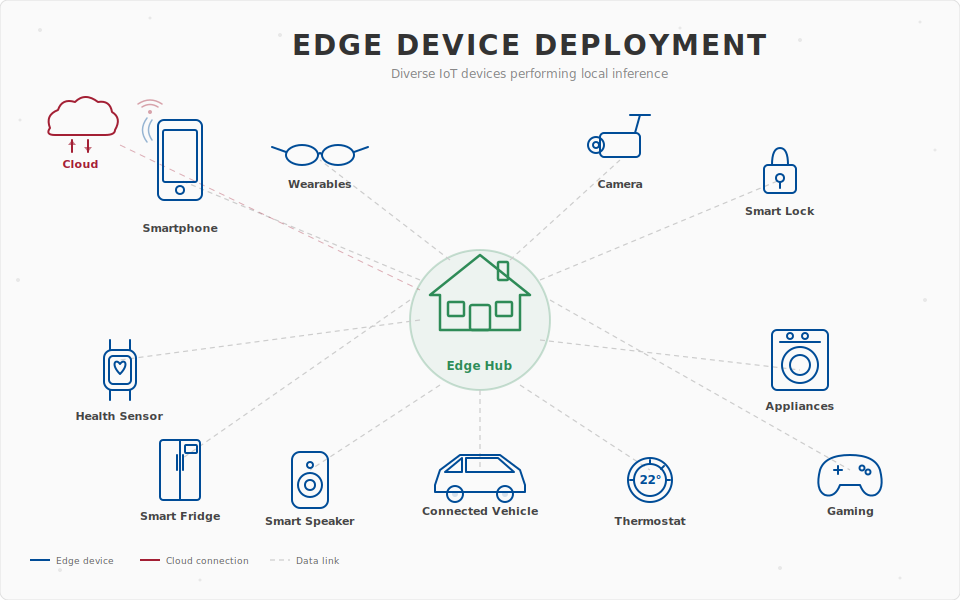
\includegraphics[keepaspectratio]{contents/vol1/ml_systems/images/jpg/edge_ml_iot.jpg}}

}

\caption{\label{fig-edgeml-example}\textbf{Edge Device Deployment}:
Diverse IoT devices, from wearables to home appliances, enable
decentralized machine learning by performing inference locally, reducing
reliance on cloud connectivity and improving response times. Source:
Edge Impulse.}

\end{figure}%

\subsection{Real-Time Industrial and IoT
Systems}\label{sec-ml-system-architecture-realtime-industrial-iot-systems-373a}

Industries deploy Edge ML widely where low latency, data privacy, and
operational resilience justify the additional complexity. Autonomous
vehicles represent the most demanding application, where safety-critical
decisions must occur within milliseconds based on sensor data that
cannot be transmitted to remote servers. Systems like Tesla's Full
Self-Driving process inputs from multiple cameras at high frame rates
through custom edge hardware, making driving decisions with end-to-end
latency on the order of milliseconds. This response time is infeasible
with cloud processing due to network delays.

Smart retail environments demonstrate edge ML's practical advantages for
privacy-sensitive, bandwidth-intensive applications. Amazon
Go\sidenote{\textbf{Amazon Go}: Launched in 2018, this checkout-free
retail concept demonstrates edge ML at scale. Each store deploys
hundreds of cameras and shelf sensors processed by local GPU clusters
running multi-object tracking, pose estimation, and activity
recognition. The system must process \textasciitilde1 TB/hour of video
data locally because cloud transmission would require impractical
bandwidth (100+ Mbps sustained) and add unacceptable latency for
real-time tracking. } stores process video from hundreds of cameras
through local edge servers, tracking customer movements and item
selections to enable checkout-free shopping. This edge-based approach
addresses both technical and privacy concerns. Transmitting
high-resolution video from hundreds of cameras would require substantial
sustained bandwidth, while local processing keeps raw video on premises,
reducing exposure and simplifying compliance.

The Industrial IoT\sidenote{\textbf{Industry 4.0}: Fourth industrial
revolution (term coined 2011 at Hannover Fair) integrating AI, IoT, and
cyber-physical systems into manufacturing. Digital twins simulate
production lines; ML optimizes scheduling and quality control. Industry
analyses project significant productivity gains and cost reductions
across global manufacturing through smart factory adoption
(\citeproc{ref-mckinsey2021iot}{McKinsey Global Institute 2021}). }
leverages edge ML for applications where millisecond-level
responsiveness directly impacts production efficiency and worker safety.
Manufacturing facilities deploy edge ML systems for real-time quality
control. Vision systems inspect welds at speeds exceeding 60 parts per
minute. Predictive maintenance\sidenote{\textbf{Predictive Maintenance}:
ML-driven maintenance scheduling analyzing vibration, temperature, and
acoustic signatures to predict equipment failures. Industry deployments
report significant reductions in unplanned downtime, maintenance costs,
and extended equipment life. Large-scale industrial IoT platforms
monitor millions of assets, demonstrating substantial savings through
failure avoidance (\citeproc{ref-mckinsey2021iot}{McKinsey Global
Institute 2021}). } applications monitor over 10,000 industrial assets
per facility. This approach has demonstrated 25-35\% reductions in
unplanned downtime across various manufacturing sectors.

Smart buildings utilize edge ML to optimize energy consumption while
maintaining operational continuity during network outages. Commercial
buildings equipped with edge-based building management systems process
data from thousands of sensors monitoring temperature, occupancy, air
quality, and energy usage. This reduces cloud transmission requirements
by an order of magnitude or more while enabling sub-second response
times. Healthcare applications similarly leverage edge ML for patient
monitoring and surgical assistance, maintaining HIPAA compliance through
local processing while supporting low-latency workflows for real-time
guidance.

\phantomsection\label{quiz-question-sec-ml-system-architecture-edge-ml-reducing-latency-privacy-risk-2625}
\begin{fbx}{callout-quiz-question}{Self-Check: Question 1.3}{}
\phantomsection\label{quiz-question-sec-ml-system-architecture-edge-ml-reducing-latency-privacy-risk-2625}

\begin{enumerate}
\def\labelenumi{\arabic{enumi}.}
\item
  Which of the following best describes a primary advantage of Edge ML
  over Cloud ML for latency-critical applications?

  \begin{enumerate}
  \def\labelenumii{\alph{enumii})}
  \tightlist
  \item
    Unlimited computational resources
  \item
    Reduced latency
  \item
    Lower initial deployment costs
  \item
    Enhanced data transmission capabilities
  \end{enumerate}
\item
  True or False: Edge ML inherently provides better data privacy than
  Cloud ML.
\item
  Discuss the trade-offs between computational resources and latency
  when choosing between Cloud ML and Edge ML for a real-time industrial
  IoT application.
\item
  Edge ML systems typically operate in the tens to hundreds of watts
  range and rely on localized hardware optimized for \_\_\_\_
  processing.
\item
  Order the following Edge ML benefits by their impact on deployment
  decisions: (1) Enhanced Data Privacy, (2) Reduced Latency, (3) Lower
  Bandwidth Usage.
\end{enumerate}

\noindent\hspace*{1.25em}\hyperref[quiz-answer-sec-ml-system-architecture-edge-ml-reducing-latency-privacy-risk-2625]{\textbf{See Answer~$\rightarrow$}}

\end{fbx}

\section{Mobile ML: Personal and Offline
Intelligence}\label{sec-ml-system-architecture-mobile-ml-personal-offline-intelligence-0983}

Edge ML solves the distance problem that limits cloud deployments,
achieving sub-100 ms latency through local processing. However, edge
devices remain tethered to stationary infrastructure---gateways, factory
servers, retail edge systems---limiting where intelligence can be
deployed. To bring ML capabilities to users in motion, we must solve a
different constraint: the \textbf{Battery}. Unlike plugged-in edge
servers that can consume hundreds of watts continuously, mobile devices
must operate for hours or days on fixed energy budgets.

Mobile ML addresses this challenge by integrating machine learning
directly into portable devices like smartphones and tablets, providing
users with real-time, personalized capabilities. This paradigm excels
when user privacy, offline operation, and immediate responsiveness
matter more than computational sophistication. Mobile ML supports
applications such as voice recognition\sidenote{\textbf{Voice
Recognition Evolution}: Apple Siri (2011) required cloud processing with
200-500ms latency and privacy concerns. By 2017, on-device models
reduced latency to \textless50ms while keeping audio local. Modern NPUs
process 16kHz audio in 20-30ms using transformer-based models; Google's
on-device transcription achieves 95\%+ accuracy entirely locally. },
computational photography\sidenote{\textbf{Computational Photography}:
Combines multiple exposures and ML algorithms to enhance image quality.
Google's Night Sight captures 15 frames in 6 seconds, using ML to align
and merge them. Portrait mode uses depth estimation ML models to create
professional-looking bokeh effects in real-time. }, and health
monitoring while maintaining data privacy through on-device computation.
These battery-powered devices must balance performance with power
efficiency and thermal management, making them ideal for frequent,
short-duration AI tasks.

The mobile environment introduces a critical constraint absent from
stationary deployments: \emph{energy per inference} becomes a
first-order design parameter. A \textbf{Compute Beast} workload like
image classification must be transformed through architectural
efficiency (e.g., depthwise separable
convolutions\sidenote{\textbf{Depthwise Separable Convolutions}:
Architectural innovation introduced by MobileNet (2017) that factorizes
standard convolutions into depthwise and pointwise operations. For a
\(D_K \times D_K\) kernel on \(M\) input channels producing \(N\)
outputs, standard convolution costs \(D_K^2 \times M \times N\)
multiplications, while depthwise separable costs
\(D_K^2 \times M + M \times N\), yielding 8-9x reduction for typical
parameters. This efficiency enables running vision models within mobile
power budgets. } in MobileNet) to reduce FLOPs by 8-9× while preserving
accuracy. This is not merely optimization --- it represents a
fundamental shift in the arithmetic intensity trade-off, accepting lower
peak throughput in exchange for sustainable operation within a 3-5 W
thermal envelope.

\phantomsection\label{callout-definitionux2a-1.10}
\begin{fbx}{callout-definition}{Definition: }{Mobile ML}
\phantomsection\label{callout-definition*-1.10}
\textbf{Mobile Machine Learning (Mobile ML)} refers to the deployment of
machine learning models directly on \emph{portable, battery-powered
devices}, enabling \emph{personalization}, \emph{privacy}, and
\emph{offline operation} within severe energy and resource constraints.

\end{fbx}

Figure~\ref{fig-mobile-ml} contrasts the unique characteristics of
mobile deployment against its enabling benefits and inherent challenges:
on-device processing and sensor integration enable real-time
responsiveness and enhanced privacy, while limited computational
resources and battery constraints demand aggressive model optimization.

\begin{figure}[htb]

\centering{

\pandocbounded{\includegraphics[keepaspectratio]{index_files/mediabag/e3d2ecf260b1ad60a61952decfc66021e8508d0d.pdf}}

}

\caption{\label{fig-mobile-ml}\textbf{Mobile ML Capabilities}: Mobile
machine learning systems balance performance with resource constraints
through on-device processing, specialized hardware acceleration, and
optimized frameworks. This figure outlines key considerations for
deploying ML models on mobile devices, including the trade-offs between
computational efficiency, battery life, and model performance.}

\end{figure}%

The battery life and resource constraints listed above translate
directly into engineering requirements. Consider the implications for
always-on ML features.

\phantomsection\label{callout-perspectiveux2a-1.11}
\begin{fbx}{callout-perspective}{Systems Perspective: }{Napkin Math: The Battery Tax}
\phantomsection\label{callout-perspective*-1.11}
\textbf{Problem}: You want to deploy a ``real-time'' background object
detector on a smartphone. The model consumes \textbf{2 Watts} of
continuous power when active. The phone has a standard \textbf{15
Watt-hour (Wh)} battery.

\textbf{The Physics}: 1. \textbf{Ideal Runtime}:
\(15 \text{ Wh} / 2 \text{ W} = \mathbf{7.5 \text{ hours}}\). 2.
\textbf{The Reality}: A user expects their phone to last 24 hours. Your
single feature has just consumed \textbf{30\%} of the entire daily
energy budget in a few hours.

\textbf{The Engineering Conclusion}: You cannot simply ``deploy'' the
model. You must use the techniques in \textbf{?@sec-model-compression}
(quantization, duty-cycling) to reduce the power to \textbf{\textless100
mW} if you want it to stay on all day.

\end{fbx}

The battery constraint limits total energy consumption over time.
However, even if we could ignore battery life---perhaps for a plugged-in
tablet or a short demo---a second physical law intervenes:
thermodynamics. Every watt of computation becomes a watt of heat that
must be dissipated. In a data center, massive cooling systems remove
this heat. In a thin, sealed mobile device with no fan, the only heat
path is through the glass and metal casing to the surrounding air. This
thermal reality creates a hard ceiling on sustained power consumption
that exists independently of battery capacity.

\phantomsection\label{callout-perspectiveux2a-1.12}
\begin{fbx}{callout-perspective}{Systems Perspective: }{Napkin Math: The Thermal Wall}
\phantomsection\label{callout-perspective*-1.12}
\textbf{Problem}: Your unoptimized LLM requires \textbf{10 W} peak
compute. Can you deploy it on a mobile device?

\textbf{The Physics}: 1. \textbf{Thermal Design Power (TDP)}: A mobile
SoC allows \(\approx \mathbf{3 \text{ W}}\) for passive cooling. 2.
\textbf{Temperature Rise}: At 10 W, the device temperature rises at
\(\approx 1^\circ\text{C}\) per second. 3. \textbf{Thermal Trip}: Within
60 seconds, the hardware reaches the \textbf{Thermal Trip Point}
(\(80^\circ\text{C}\)), triggering OS throttling. 4. \textbf{The
Result}: Your 100 FPS model suddenly drops to \textbf{30 FPS} to avoid
melting the hardware.

\textbf{The Engineering Conclusion}: Quantization from FP32 to INT8
reduces power by approximately 4×, but if the baseline power is 12W, you
are still at 3W---the absolute limit of the hardware. Physics sets a
hard ceiling that no optimization can exceed.

\end{fbx}

\subsection{Battery and Thermal
Constraints}\label{sec-ml-system-architecture-battery-thermal-constraints-ab51}

Mobile devices exemplify intermediate constraints: 8-24GB RAM (varying
from mid-range to flagship), 128GB-1TB storage, 1-10 TOPS AI compute
through Neural Processing Units\sidenote{\textbf{Neural Processing Unit
(NPU)}: Specialized processors optimized for efficient neural network
inference on mobile devices. NPUs achieve high inference performance
within tight power budgets, enabling on-device AI. We examine NPU
architectures and their performance characteristics in
\textbf{?@sec-ai-acceleration}. } consuming 3-5W power. System-on-Chip
architectures\sidenote{\textbf{Mobile System-on-Chip (SoC)}:
Heterogeneous processors integrating CPU, GPU, NPU, ISP, and memory
controller on a single die. Apple's A17 Pro (3nm, 19B transistors)
delivers 35 TOPS via its 16-core Neural Engine; Qualcomm's Snapdragon 8
Gen 3 delivers approximately 34 TOPS through its Hexagon NPU. SoC
integration reduces data movement energy 10-100× compared to discrete
components. } integrate computation and memory to minimize energy costs.
Memory bandwidth of 25-50 GB/s limits models to 10-100MB parameters,
requiring the aggressive optimization techniques that
\textbf{?@sec-model-compression} details. Battery constraints (18-22Wh
capacity) make energy optimization critical: 1W continuous ML processing
reduces device lifetime from 24 to 18 hours. Specialized frameworks
(TensorFlow Lite\sidenote{\textbf{TensorFlow Lite}: Google's
mobile/embedded ML framework (2017) optimizing models through
quantization, pruning, and operator fusion. Supports Android, iOS,
Linux, and microcontrollers. Deploys on 4B+ devices running applications
from Google Translate (35MB multilingual model) to on-device speech
recognition with \textless100ms latency. }, Core
ML\sidenote{\textbf{Core ML}: Apple's on-device ML framework (iOS 11,
2017) with automatic optimization for Apple Silicon. Seamlessly
schedules across CPU, GPU, and Neural Engine based on model
characteristics. Supports vision, NLP, and audio models from 1 KB--1 GB
with compiler optimizations achieving 2--10\(\times\) speedups over
naive deployment. }) provide hardware-optimized inference enabling
\textless50ms UI response times.

\subsection{Mobile ML Benefits and Resource
Constraints}\label{sec-ml-system-architecture-mobile-ml-benefits-resource-constraints-c568}

Mobile ML excels at delivering responsive, privacy-preserving user
experiences. Real-time processing can reach sub-10 ms latency for some
tasks, enabling imperceptible response in interactive applications.
Stronger privacy properties emerge when sensitive inputs are processed
locally, reducing data transmission and central storage, though privacy
still depends on system design and threat model. On-device enclaves and
similar hardware isolation mechanisms can help protect sensitive
computations (for example, biometric processing)\sidenote{\textbf{Mobile
Face Detection}: Apple's Face ID projects 30,000 IR dots for 3D face
mapping, processed entirely in the Secure Enclave (isolated
cryptographic coprocessor). Biometric templates never leave the device;
even Apple cannot access them. Achieves 1:1,000,000 false acceptance
rate vs.~Touch ID's 1:50,000, demonstrating privacy-preserving edge AI.
}. Offline functionality reduces network dependency: navigation,
translation\sidenote{\textbf{Real-Time Translation}: On-device neural
machine translation processing 40+ language pairs without internet
connectivity. Google Translate's offline models (35-45MB per language)
achieve 90\% of cloud quality (2GB+ models) through knowledge
distillation and quantization. Enables privacy-preserving translation
with \textless500ms latency on mid-range smartphones. }, and media
processing can run locally within mobile resource budgets.
Personalization improves because models can leverage on-device signals
and user context while keeping raw data local.

These benefits require accepting significant resource constraints.
Compared to cloud deployments, mobile applications often operate under
much tighter memory, storage, and latency budgets, which constrains
model size and batch behavior. Battery life\sidenote{\textbf{Mobile
Device Constraints}: Flagship phones (12-24GB RAM, 15-25W peak power)
operate with 10-100× less resources than cloud servers (256-2048GB RAM,
200-400W). Thermal throttling limits sustained performance; battery life
requires \textless500mW average inference power. These constraints drove
innovations in efficient architectures (MobileNet, EfficientNet) and
on-device optimization. } presents visible user impact, and thermal
throttling can materially limit sustained performance: peak NPU
throughput is often substantially higher than what is sustainable under
prolonged workloads. Development complexity multiplies across platforms,
demanding separate implementations and careful performance tuning, while
device heterogeneity requires multiple model variants. Deployment
friction adds further challenges: app store review processes can take
days, which can slow iteration relative to many cloud deployment
workflows.

\subsection{Personal Assistant and Media
Processing}\label{sec-ml-system-architecture-personal-assistant-media-processing-98d7}

Mobile ML has achieved success across diverse applications for billions
of users worldwide. Computational photography transformed smartphone
cameras into sophisticated imaging systems. Modern flagships process
every photo through multiple ML pipelines operating in real-time:
portrait mode\sidenote{\textbf{Portrait Mode Photography}: Computational
photography using ML segmentation to separate subjects from backgrounds,
applying synthetic depth-of-field effects mimicking DSLR bokeh. Dual
cameras or LiDAR provide depth estimation; neural networks refine edges
around hair and translucent objects. Processing occurs in real-time
(\textless100ms) on NPUs, enabling live preview before capture. } uses
depth estimation and segmentation networks to achieve DSLR-quality bokeh
effects, night mode captures and aligns 9-15 frames with ML-based
denoising that reduces noise by 10-20dB, and systems like Google Pixel
process 10-15 distinct ML models per photo for HDR merging,
super-resolution, and scene optimization.

Voice-driven interactions demonstrate mobile ML's transformation of
human-device communication. These systems combine ultra-low-power
wake-word detection consuming less than 1mW with on-device speech
recognition achieving under 10ms latency for simple commands. Keyboard
prediction has evolved to context-aware neural models achieving 60-70\%
phrase prediction accuracy, reducing typing effort by 30-40\%. Real-time
camera translation processes over 100 languages at 15-30fps entirely
on-device, enabling instant visual translation without internet
connectivity.

Health monitoring through wearables like Apple Watch extracts
sophisticated insights from sensor data while maintaining complete
privacy. These systems achieve over 95\% accuracy in activity detection
and include FDA-cleared atrial fibrillation detection with 98\%+
sensitivity, processing extraordinarily sensitive health data entirely
on-device to maintain HIPAA compliance. Accessibility features
demonstrate transformative social impact through continuous local
processing: Live Text detects and recognizes text from camera feeds,
Sound Recognition alerts deaf users to environmental cues through haptic
feedback, and VoiceOver generates natural language descriptions of
visual content.

Augmented reality frameworks leverage mobile ML for real-time
environment understanding at 60fps. ARCore and ARKit track device
position with centimeter-level accuracy while simultaneously mapping 3D
surroundings, enabling hand tracking that extracts 21-joint 3D poses and
face analysis of 50+ landmark meshes for real-time effects. These
applications demand consistent sub-16ms frame times, making only
on-device processing viable for delivering the seamless experiences
users expect.

Despite mobile ML's demonstrated capabilities, a common pitfall involves
attempting to deploy desktop-trained models directly to mobile or edge
devices without architecture modifications. Models developed on powerful
workstations often fail when deployed to resource-constrained devices. A
ResNet-50 model requiring 4 GB memory for inference (including
activations and batch processing) and 4 billion FLOPs per inference
cannot run on a device with 512 MB of RAM and a 1 GFLOP/s processor.
Beyond simple resource violations, desktop-optimized models may use
operations unsupported by mobile hardware (specialized mathematical
operations), assume floating-point precision unavailable on embedded
systems, or require batch processing incompatible with single-sample
inference. Successful deployment demands architecture-aware design from
the beginning, including specialized architectural techniques for mobile
devices (\citeproc{ref-howard2017mobilenets}{Howard et al. 2017}),
integer-only operations for microcontrollers, and optimization
strategies that maintain accuracy while reducing computation.

\phantomsection\label{quiz-question-sec-ml-system-architecture-mobile-ml-personal-offline-intelligence-0983}
\begin{fbx}{callout-quiz-question}{Self-Check: Question 1.4}{}
\phantomsection\label{quiz-question-sec-ml-system-architecture-mobile-ml-personal-offline-intelligence-0983}

\begin{enumerate}
\def\labelenumi{\arabic{enumi}.}
\item
  Which of the following best describes a primary advantage of Mobile ML
  over Edge ML?

  \begin{enumerate}
  \def\labelenumii{\alph{enumii})}
  \tightlist
  \item
    Greater computational power
  \item
    Improved user privacy and offline functionality
  \item
    Reduced hardware costs
  \item
    Higher data storage capacity
  \end{enumerate}
\item
  Discuss the trade-offs involved in deploying machine learning models
  on mobile devices compared to cloud-based systems.
\item
  True or False: Mobile ML can achieve the same level of computational
  sophistication as cloud-based ML systems.
\item
  In a production system, which application is most suited for Mobile ML
  deployment?

  \begin{enumerate}
  \def\labelenumii{\alph{enumii})}
  \tightlist
  \item
    Real-time voice recognition
  \item
    Large-scale data analytics
  \item
    Complex neural network training
  \item
    Batch processing of large datasets
  \end{enumerate}
\end{enumerate}

\noindent\hspace*{1.25em}\hyperref[quiz-answer-sec-ml-system-architecture-mobile-ml-personal-offline-intelligence-0983]{\textbf{See Answer~$\rightarrow$}}

\end{fbx}

\section{TinyML: Ubiquitous Sensing at
Scale}\label{sec-ml-system-architecture-tinyml-ubiquitous-sensing-scale-a67b}

Mobile ML brings intelligence to users on the move, but smartphones cost
hundreds to thousands of dollars and are far too large to embed in
everyday objects. To put ``eyes and ears'' on every physical
object---from individual boxes in a warehouse to every leaf in a
field---we must push beyond mobile constraints entirely, solving for
both \textbf{cost} (dollars, not hundreds of dollars) and \textbf{size}
(millimeters, not centimeters).

TinyML completes the deployment spectrum by pushing intelligence to its
physical limits. Devices costing less than \$10 and consuming less than
1 milliwatt of power make ubiquitous\sidenote{\textbf{Ubiquitous}: From
Latin \emph{ubique} (everywhere), combining \emph{ubi} (where) and the
generalizing suffix \emph{-que}. Mark Weiser at Xerox PARC coined
``ubiquitous computing'' in 1988 to describe technology so embedded in
the environment that it becomes invisible. TinyML realizes this vision:
when sensors cost dollars and run for years on a battery, intelligence
can literally be \emph{everywhere}, disappearing into the physical
world. } sensing economically practical at massive scale. This is the
exclusive domain of the \textbf{Tiny Constraint} Archetype, where the
optimization objective shifts from maximizing throughput to minimizing
energy per inference --- a keyword spotting model consuming 10 µJ per
inference can operate for years on a coin-cell battery, achieving
million-fold improvements in energy efficiency by trading model capacity
for operational longevity.

Where mobile ML requires sophisticated hardware with gigabytes of memory
and multi-core processors, Tiny Machine Learning operates on
microcontrollers with kilobytes of RAM and single-digit dollar price
points. This radical constraint forces a shift in machine learning
deployment, prioritizing ultra-low power consumption and minimal cost
over computational sophistication.

TinyML brings intelligence to the smallest devices, from
microcontrollers\sidenote{\textbf{Microcontrollers}: Single-chip
computers with integrated CPU, memory, and peripherals, typically
operating at 1-100MHz with 32KB-2MB RAM. Arduino Uno uses an ATmega328P
with 32KB flash and 2KB RAM, while ESP32 provides WiFi capability with
520KB RAM, still thousands of times less than a smartphone. } to
embedded sensors, enabling real-time computation in severely
resource-constrained environments. This paradigm excels in applications
requiring ubiquitous sensing, autonomous operation, and maximal energy
efficiency. TinyML systems power applications such as predictive
maintenance, environmental monitoring, and simple gesture recognition
while optimized for energy efficiency\sidenote{\textbf{Energy Efficiency
in TinyML}: Ultra-low power enables decade-long deployment in remote
locations. ARM Cortex-M0+ consumes \textless1µW in sleep, 100-300µW/MHz
active. Specialized accelerators (Syntiant NDP, MAX78000) achieve
\textless1µJ per inference. This 1,000,000\(\times\) gap between TinyML
and cloud inference energy drives entirely different system
architectures and deployment models. }, often running for months or
years on limited power sources such as coin-cell
batteries\sidenote{\textbf{Coin-Cell Batteries}: Compact power sources
(CR2032: 225mAh at 3V) enabling ``deploy-and-forget'' IoT devices.
TinyML models consuming 10-50µW average power can operate 1-10 years on
a single cell. Constrains models to \textless100KB (fitting in on-chip
SRAM), driving innovation in efficient neural network architectures and
intermittent computing paradigms. }, as exemplified by the device kits
in Figure~\ref{fig-TinyML-example}. These systems deliver actionable
insights in remote or disconnected environments where power,
connectivity, and maintenance access are impractical.

\phantomsection\label{callout-definitionux2a-1.13}
\begin{fbx}{callout-definition}{Definition: }{TinyML}
\phantomsection\label{callout-definition*-1.13}
\textbf{Tiny Machine Learning (TinyML)} refers to the deployment of
machine learning models on \emph{microcontrollers} and
\emph{ultra-constrained devices}, enabling \emph{autonomous
decision-making} with milliwatt-scale power consumption for applications
requiring years of battery life.

\end{fbx}

The ``milliwatt-scale power consumption'' in this definition represents
a six-order-of-magnitude reduction from cloud inference---a gap with
profound implications for system design.

\begin{tcolorbox}[enhanced jigsaw, coltitle=black, opacitybacktitle=0.6, colback=white, toprule=.15mm, rightrule=.15mm, arc=.35mm, bottomtitle=1mm, title=\textcolor{quarto-callout-note-color}{\faInfo}\hspace{0.5em}{Energy Per Inference: The Million-Fold Gap}, toptitle=1mm, colframe=quarto-callout-note-color-frame, breakable, titlerule=0mm, bottomrule=.15mm, leftrule=.75mm, left=2mm, opacityback=0, colbacktitle=quarto-callout-note-color!10!white]

Energy consumption spans six orders of magnitude across deployment
paradigms:

\begin{longtable}[]{@{}
  >{\raggedright\arraybackslash}p{(\linewidth - 6\tabcolsep) * \real{0.1531}}
  >{\raggedright\arraybackslash}p{(\linewidth - 6\tabcolsep) * \real{0.2347}}
  >{\raggedleft\arraybackslash}p{(\linewidth - 6\tabcolsep) * \real{0.2347}}
  >{\raggedleft\arraybackslash}p{(\linewidth - 6\tabcolsep) * \real{0.3571}}@{}}
\toprule\noalign{}
\begin{minipage}[b]{\linewidth}\raggedright
\textbf{Paradigm}
\end{minipage} & \begin{minipage}[b]{\linewidth}\raggedright
\textbf{Example Workload}
\end{minipage} & \begin{minipage}[b]{\linewidth}\raggedleft
\textbf{Energy/Inference}
\end{minipage} & \begin{minipage}[b]{\linewidth}\raggedleft
\textbf{Battery Life (3.7V, 3000mAh)}
\end{minipage} \\
\midrule\noalign{}
\endhead
\bottomrule\noalign{}
\endlastfoot
\textbf{Cloud} & GPT-4 query & \textasciitilde1 kJ & 0.01 queries \\
\textbf{Cloud} & ResNet-50 (A100) & \textasciitilde10 J & 1 query \\
\textbf{Edge} & ResNet-50 (Jetson) & \textasciitilde500 mJ & 20
queries \\
\textbf{Mobile} & MobileNet (NPU) & \textasciitilde50 mJ & 200
queries \\
\textbf{TinyML} & Keyword spotting & \textasciitilde10 µJ & 1 billion
inferences \\
\end{longtable}

\textbf{Key insight}: A TinyML wake-word detector at 10 µJ/inference is
\textbf{100,000,000×} more energy-efficient than a cloud LLM query. This
gap explains why always-on sensing is only practical at the TinyML
tier---a smartphone running continuous cloud queries would drain in
minutes.

\end{tcolorbox}

Figure~\ref{fig-tiny-ml} maps TinyML's unique position at the
resource-constrained extreme of the deployment spectrum, where milliwatt
power budgets and kilobyte memory limits transform algorithmic
possibilities: the paradigm achieves extremely low latency and always-on
operation but demands specialized model compression techniques that
fundamentally reshape what ML can accomplish.

\begin{figure}[htb]

\centering{

\pandocbounded{\includegraphics[keepaspectratio]{index_files/mediabag/702702e3d82fdd3798e40a50b32ca8b8c81dcfec.pdf}}

}

\caption{\label{fig-tiny-ml}\textbf{TinyML System Characteristics}:
Constrained devices necessitate a focus on efficiency, driving
trade-offs between model complexity, accuracy, and energy consumption,
while enabling localized intelligence and real-time responsiveness in
embedded applications. This figure outlines key aspects of TinyML,
including the challenges of resource limitations, example applications,
and the benefits of on-device machine learning.}

\end{figure}%

\subsection{Extreme Resource
Constraints}\label{sec-ml-system-architecture-extreme-resource-constraints-2273}

TinyML operates at hardware extremes. Compared to cloud systems, TinyML
deployments often have on the order of (10\^{}4) to (10\^{}5) times less
memory and power budgets in the milliwatt range. Such strict limitations
enable months or years of autonomous
operation\sidenote{\textbf{On-Device Training Constraints}:
Microcontrollers (256KB-2MB RAM) cannot support full backpropagation
through large networks. Alternatives include on-device fine-tuning of
final layers, federated learning with local gradient computation, and
TinyTL (memory-efficient training using \textless50KB). Apple's
on-device personalization adapts keyboard predictions without uploading
typing data. } but demand specialized algorithms and careful systems
co-design. Devices range from palm-sized developer kits to
millimeter-scale chips\sidenote{\textbf{TinyML Device Scale}: ML-capable
chips range from 5×5mm (Syntiant NDP: 140µW, 1MB SRAM) to full
single-board computers (Coral Dev Board Mini: 40×48mm, 4 TOPS). This
100× size range reflects diverse deployment needs from implantable
medical devices to industrial edge gateways processing multiple sensor
streams simultaneously. }, enabling ubiquitous sensing in contexts where
networking, power, or maintenance are costly. Representative developer
kits include the Arduino Nano 33 BLE Sense (256KB RAM, 1MB flash,
20-40mW) and ESP32-CAM (520KB RAM, 4MB flash, 50-250mW).

\begin{figure}

\centering{

\pandocbounded{\includegraphics[keepaspectratio]{contents/vol1/ml_systems/images/png/tiny_ml.png}}

}

\caption{\label{fig-TinyML-example}\textbf{TinyML System Scale}: These
device kits exemplify the extreme miniaturization achievable with
TinyML, enabling deployment of machine learning on resource-constrained
devices with limited power and memory. Such compact systems broaden the
applicability of ML to previously inaccessible edge applications,
including wearable sensors and embedded IoT devices. Source:
(\citeproc{ref-warden2018speech}{Warden 2018})}

\end{figure}%

\subsection{TinyML Advantages and Operational
Trade-offs}\label{sec-ml-system-architecture-tinyml-advantages-operational-tradeoffs-2d40}

TinyML's extreme resource constraints enable unique advantages that are
difficult to achieve at other scales. Avoiding network transmission
reduces end-to-end latency and eliminates communication overhead,
enabling rapid local responses for sensing and control loops. The
economics can be compelling for massive-scale deployments because
per-node costs can be low enough to instrument large physical
environments. Energy efficiency enables multi-year operation on small
batteries, and energy harvesting can further extend lifetimes in some
settings. Privacy improves because raw data can remain local, reducing
transmission and central storage, though this does not automatically
provide formal privacy guarantees without additional privacy and
security mechanisms.

These capabilities require substantial trade-offs. Computational
constraints impose severe limits: microcontrollers commonly provide on
the order of (10\^{}5) to (10\^{}6) bytes of RAM, which can force models
and intermediate activations into the tens of kilobytes to low megabytes
range, depending on the workload. Development complexity requires
expertise spanning neural network optimization, hardware-level memory
management, embedded toolchains, and specialized debugging across
diverse microcontroller architectures. Model quality can suffer from
aggressive compression and reduced precision, limiting suitability for
applications requiring high accuracy or robustness. Deployment can also
be inflexible: devices may run a small set of fixed models, and updates
may require firmware workflows that are slower and riskier than cloud
rollouts. Ecosystem fragmentation\sidenote{\textbf{TinyML Model
Optimization}: Compression techniques enable running ML on
microcontrollers by dramatically reducing model size while preserving
accuracy. Quantization, pruning, knowledge distillation, and
architecture search work together to achieve these reductions. Detailed
compression methods are covered in \textbf{?@sec-model-compression}. }
across microcontroller vendors and ML frameworks creates additional
overhead and portability challenges.

\subsection{Environmental and Health
Monitoring}\label{sec-ml-system-architecture-environmental-health-monitoring-14ad}

TinyML succeeds across domains where its advantages of ultra-low power,
low per-node cost, and local processing enable applications impractical
with other paradigms.

Wake-word detection represents a visible consumer application of TinyML,
where always-listening capabilities can be implemented at sub-milliwatt
continuous power consumption. These systems typically process audio
streams locally and only activate higher-power components when a wake
phrase is detected, reducing average device power
draw\sidenote{\textbf{TinyML in Fitness Trackers}: Wearables run
continuous ML inference on accelerometer, gyroscope, and heart rate
data. Apple Watch's fall detection analyzes motion patterns at 50Hz,
distinguishing falls from sitting down with high accuracy. Operating at
\textless1mW enables week-long battery life while monitoring health
metrics 24/7, a defining example of always-on TinyML. }.

Precision agriculture leverages TinyML's economic advantages where
traditional solutions prove cost-prohibitive. Deployments can instrument
thousands of monitoring points with multi-year battery operation,
transmitting summaries instead of raw sensor streams to reduce
connectivity costs.

Wildlife conservation uses TinyML for remote environmental monitoring.
Researchers deploy solar-powered audio sensors consuming 100-500mW that
process continuous audio streams for species identification. By
performing local analysis, these systems reduce satellite transmission
requirements from 4.3GB per day to 400KB of detection summaries, a
10,000x reduction that makes large-scale deployments of 100-1,000
sensors economically feasible. Medical wearables achieve FDA-cleared
cardiac monitoring with 95-98\% sensitivity while processing 250-500 ECG
samples per second at under 5mW power consumption. This efficiency
enables week-long continuous monitoring versus hours for
smartphone-based alternatives, while reducing diagnostic costs from
\$2,000-5,000 for traditional in-lab studies to under \$100 for at-home
testing.

\phantomsection\label{quiz-question-sec-ml-system-architecture-tinyml-ubiquitous-sensing-scale-a67b}
\begin{fbx}{callout-quiz-question}{Self-Check: Question 1.5}{}
\phantomsection\label{quiz-question-sec-ml-system-architecture-tinyml-ubiquitous-sensing-scale-a67b}

\begin{enumerate}
\def\labelenumi{\arabic{enumi}.}
\item
  Which of the following best describes a primary advantage of Tiny ML
  over Mobile ML?

  \begin{enumerate}
  \def\labelenumii{\alph{enumii})}
  \tightlist
  \item
    Higher computational power
  \item
    Increased data storage capacity
  \item
    Greater model accuracy
  \item
    Lower deployment cost and power consumption
  \end{enumerate}
\item
  Discuss the trade-offs involved in deploying Tiny ML systems in remote
  environments.
\item
  Tiny ML enables applications that require \_\_\_\_\_\_\_\_ decision
  making in resource-constrained environments.
\item
  True or False: Tiny ML systems can achieve the same level of model
  accuracy as cloud-based systems.
\item
  In a production system, which application is most suited for Tiny ML
  deployment?

  \begin{enumerate}
  \def\labelenumii{\alph{enumii})}
  \tightlist
  \item
    Environmental monitoring
  \item
    Real-time language translation
  \item
    High-frequency stock trading
  \item
    3D rendering
  \end{enumerate}
\end{enumerate}

\noindent\hspace*{1.25em}\hyperref[quiz-answer-sec-ml-system-architecture-tinyml-ubiquitous-sensing-scale-a67b]{\textbf{See Answer~$\rightarrow$}}

\end{fbx}

\section{Comparative Analysis and Paradigm
Selection}\label{sec-ml-system-architecture-comparative-analysis-paradigm-selection-bf66}

The preceding four sections examined each deployment paradigm through
the same lens: definition, characteristics, trade-offs, and
applications. This parallel treatment revealed that each paradigm
emerged as a response to specific physical constraints---Cloud ML
accepts latency for unlimited compute, Edge ML trades compute for
latency, Mobile ML trades compute for portability, and TinyML trades
compute for ubiquity.

Now we step back to see the full picture. How do these paradigms compare
quantitatively across all dimensions? And given a specific application,
how should an engineer select among them? This section synthesizes the
individual paradigm analyses into a unified comparison framework and a
structured decision process.

\subsection{Quantitative Trade-off
Analysis}\label{sec-ml-system-architecture-quantitative-tradeoff-analysis-56a8}

The relationship between computational resources and deployment location
forms one of the most important comparisons across ML systems. As we
move from cloud deployments to tiny devices, we observe a dramatic
reduction in available computing power, storage, and energy consumption.
Cloud ML systems, with their data center infrastructure, can leverage
virtually unlimited resources, processing data at the scale of petabytes
and training models with billions of parameters. Edge ML systems, while
more constrained, still offer significant computational capability
through specialized hardware like edge GPUs and neural processing units.
Mobile ML represents a middle ground, balancing computational power with
energy efficiency on devices like smartphones and tablets. At the far
end of the spectrum, TinyML operates under severe resource constraints,
often limited to kilobytes of memory and milliwatts of power
consumption.

Table~\ref{tbl-big_vs_tiny} provides a comprehensive comparison across
performance, operational, and deployment dimensions.

\begin{longtable}[]{@{}
  >{\raggedright\arraybackslash}p{(\linewidth - 8\tabcolsep) * \real{0.1422}}
  >{\raggedright\arraybackslash}p{(\linewidth - 8\tabcolsep) * \real{0.2108}}
  >{\raggedright\arraybackslash}p{(\linewidth - 8\tabcolsep) * \real{0.2010}}
  >{\raggedright\arraybackslash}p{(\linewidth - 8\tabcolsep) * \real{0.1569}}
  >{\raggedright\arraybackslash}p{(\linewidth - 8\tabcolsep) * \real{0.2745}}@{}}
\caption{\textbf{Deployment Locations}: Machine learning systems vary in
where computation occurs, from centralized cloud servers to local edge
devices and ultra-low-power TinyML chips, each impacting latency,
bandwidth, and energy consumption. This table categorizes these
deployments by their processing location and associated characteristics,
enabling informed decisions about system architecture and resource
allocation.}\label{tbl-big_vs_tiny}\tabularnewline
\toprule\noalign{}
\begin{minipage}[b]{\linewidth}\raggedright
\textbf{Aspect}
\end{minipage} & \begin{minipage}[b]{\linewidth}\raggedright
\textbf{Cloud ML}
\end{minipage} & \begin{minipage}[b]{\linewidth}\raggedright
\textbf{Edge ML}
\end{minipage} & \begin{minipage}[b]{\linewidth}\raggedright
\textbf{Mobile ML}
\end{minipage} & \begin{minipage}[b]{\linewidth}\raggedright
\textbf{TinyML}
\end{minipage} \\
\midrule\noalign{}
\endfirsthead
\toprule\noalign{}
\begin{minipage}[b]{\linewidth}\raggedright
\textbf{Aspect}
\end{minipage} & \begin{minipage}[b]{\linewidth}\raggedright
\textbf{Cloud ML}
\end{minipage} & \begin{minipage}[b]{\linewidth}\raggedright
\textbf{Edge ML}
\end{minipage} & \begin{minipage}[b]{\linewidth}\raggedright
\textbf{Mobile ML}
\end{minipage} & \begin{minipage}[b]{\linewidth}\raggedright
\textbf{TinyML}
\end{minipage} \\
\midrule\noalign{}
\endhead
\bottomrule\noalign{}
\endlastfoot
\textbf{Performance} & & & & \\
\textbf{Processing Location} & Centralized cloud servers (Data Centers)
& Local edge devices (gateways, servers) & Smartphones and tablets &
Ultra-low-power microcontrollers and embedded systems \\
\textbf{Latency} & High (100 ms-1000 ms+) & Moderate (10-100 ms) &
Low-Moderate (5-50 ms) & Very Low (1-10 ms) \\
\textbf{Compute Power} & Very High (Multiple GPUs/TPUs) & High (Edge
GPUs) & Moderate (Mobile NPUs/GPUs) & Very Low (MCU/tiny processors) \\
\textbf{Storage Capacity} & Unlimited (petabytes+) & Large (terabytes) &
Moderate (gigabytes) & Very Limited (kilobytes-megabytes) \\
\textbf{Energy Consumption} & Very High (kW-MW range) & High (100 s W) &
Moderate (1-10 W) & Very Low (mW range) \\
\textbf{Scalability} & Excellent (virtually unlimited) & Good (limited
by edge hardware) & Moderate (per-device scaling) & Limited (fixed
hardware) \\
\textbf{Operational} & & & & \\
\textbf{Data Privacy} & Basic-Moderate (Data leaves device) & High (Data
stays in local network) & High (Data stays on phone) & Very High (Raw
data can remain local) \\
\textbf{Connectivity Required} & Constant high-bandwidth & Intermittent
& Optional & None \\
\textbf{Offline Capability} & None & Good & Excellent & Complete \\
\textbf{Real-time Processing} & Dependent on network & Good & Very Good
& Excellent \\
\textbf{Deployment} & & & & \\
\textbf{Cost} & High (\$1000s+/month) & Moderate (\$100s-1000s) & Low
(\$0-10s) & Very Low (\$1-10s) \\
\textbf{Hardware Requirements} & Cloud infrastructure & Edge
servers/gateways & Modern smartphones & MCUs/embedded systems \\
\textbf{Development Complexity} & High (cloud expertise needed) &
Moderate-High (edge+networking) & Moderate (mobile SDKs) & High
(embedded expertise) \\
\textbf{Deployment Speed} & Fast & Moderate & Fast & Slow \\
\end{longtable}

Table~\ref{tbl-big_vs_tiny} reveals clear gradients in latency from
cloud (100-1000ms) to edge (10-100ms) to mobile (5-50ms) to tiny
(1-10ms), and privacy properties that are often strongest when TinyML
keeps raw data local. Before we visualize these trade-offs graphically,
let us understand how they connect to the Workload Archetypes introduced
earlier.

These quantitative trade-offs map directly to the Workload Archetypes
introduced earlier. \textbf{Compute Beasts} and \textbf{Sparse Scatter}
workloads naturally gravitate toward cloud deployment, where raw TFLOPS
and memory capacity are abundant. \textbf{Bandwidth Hogs} span cloud and
edge depending on latency requirements --- cloud for batch processing,
edge for interactive applications. \textbf{Tiny Constraint} workloads
are exclusively TinyML, where the joules-per-inference metric dominates
all other considerations. Mobile deployment occupies the middle ground,
hosting efficiency-optimized variants of Compute Beast workloads (e.g.,
MobileNet instead of ResNet) that trade peak performance for sustainable
power consumption.

Figure~\ref{fig-op_char} visualizes performance and operational
characteristics across paradigms through radar plots. Plot a) contrasts
compute power and scalability where Cloud ML excels against latency and
energy efficiency where TinyML dominates, with Edge and Mobile ML
occupying intermediate positions.

\begin{figure}[htb]

\centering{

\pandocbounded{\includegraphics[keepaspectratio]{index_files/mediabag/69761f19ef03e10519618318f80cc6704f3f55f0.pdf}}

}

\caption{\label{fig-op_char}\textbf{ML System Trade-Offs}: Radar plots
quantify performance and operational characteristics across cloud, edge,
mobile, and TinyML paradigms, revealing inherent trade-offs between
compute power, latency, energy consumption, and scalability. These
visualizations enable informed selection of the most suitable deployment
approach based on application-specific constraints and priorities.}

\end{figure}%

Plot b) emphasizes operational dimensions where TinyML excels (privacy,
connectivity independence, offline capability) versus Cloud ML's
dependency on centralized infrastructure and constant connectivity.

Development complexity varies inversely with hardware capability: Cloud
and TinyML require deep expertise (cloud infrastructure and embedded
systems respectively), while Mobile and Edge leverage more accessible
SDKs and tooling. Cost structures show similar inversion: Cloud incurs
ongoing operational expenses (\$1000s+/month), Edge requires moderate
upfront investment (\$100s-1000s), Mobile leverages existing devices
(\$0-10s), and TinyML minimizes hardware costs (\$1-10s) while demanding
higher development investment.

Understanding these trade-offs is crucial for selecting appropriate
deployment strategies.

A critical pitfall in deployment selection involves choosing paradigms
based solely on model accuracy metrics without considering system-level
constraints. Teams often select deployment strategies by comparing model
accuracy in isolation, overlooking critical system requirements that
determine real-world viability. A cloud-deployed model achieving 99\%
accuracy becomes useless for autonomous emergency braking if network
latency exceeds reaction time requirements. Similarly, a sophisticated
edge model that drains a mobile device's battery in minutes fails
despite superior accuracy. Successful deployment requires evaluating
multiple dimensions simultaneously: latency requirements, power budgets,
network reliability, data privacy regulations, and total cost of
ownership. Establish these constraints before model development to avoid
expensive architectural pivots late in the project.

\subsection{Decision
Framework}\label{sec-ml-system-architecture-decision-framework-241f}

Selecting the appropriate deployment paradigm requires systematic
evaluation of application constraints rather than organizational biases
or technology trends. Figure~\ref{fig-mlsys-playbook-flowchart} provides
a hierarchical decision framework that filters options through critical
requirements: privacy, latency, computational demands, and cost
constraints.

\begin{figure}[!t]

\centering{

\pandocbounded{\includegraphics[keepaspectratio]{index_files/mediabag/f8a9cfffda798ba0fb76197385f8913898fe02d6.pdf}}

}

\caption{\label{fig-mlsys-playbook-flowchart}\textbf{Deployment Decision
Logic}: This flowchart guides selection of an appropriate machine
learning deployment paradigm by systematically evaluating privacy
requirements and processing constraints, ultimately balancing
performance, cost, and data security. Navigating the decision tree helps
practitioners determine whether cloud, edge, mobile, or tiny machine
learning best suits a given application.}

\end{figure}%

The framework evaluates four critical decision layers sequentially.
Privacy constraints form the first filter, determining whether data can
be transmitted externally. Applications handling sensitive data under
GDPR, HIPAA, or proprietary restrictions mandate local processing,
immediately eliminating cloud-only deployments. Latency requirements
establish the second constraint through response time budgets:
applications requiring sub-10 ms response times cannot use cloud
processing, as physics-imposed network delays alone exceed this
threshold. Computational demands form the third evaluation layer,
assessing whether applications require high-performance infrastructure
that only cloud or edge systems provide, or whether they can operate
within the resource constraints of mobile or tiny devices. Cost
considerations complete the framework by balancing capital expenditure,
operational expenses, and energy efficiency across expected deployment
lifetimes.

\phantomsection\label{callout-notebook-1.5}
\begin{fbx}{callout-notebook}{AI Engineer’s Notebook 1.5: }{Worked Example: Autonomous Vehicle Emergency Braking}
\phantomsection\label{callout-notebook-1.5}
\textbf{Application}: Vision-based pedestrian detection for emergency
braking.

\textbf{Walking through the decision framework}:

\begin{enumerate}
\def\labelenumi{\arabic{enumi}.}
\item
  \textbf{Privacy}: Vehicle camera data is not transmitted to third
  parties → No strong privacy constraint. \emph{Could use cloud.}
\item
  \textbf{Latency}: Emergency braking requires \textless100 ms total
  response. At 60 mph, a car travels 2.7 meters in 100 ms.

  \begin{itemize}
  \tightlist
  \item
    Network latency to cloud: 50-150 ms (variable) → \textbf{Fails
    requirement}
  \item
    Edge processing: 10-30 ms → \textbf{Passes}
  \item
    \emph{Decision: Cloud eliminated by physics.}
  \end{itemize}
\item
  \textbf{Compute}: Pedestrian detection requires \textasciitilde10
  GFLOPs at 30 FPS = 300 GFLOPs/s sustained.

  \begin{itemize}
  \tightlist
  \item
    TinyML (\textless1 GFLOP/s): \textbf{Fails}
  \item
    Mobile NPU (\textasciitilde35 TOPS): Possible but thermal
    constraints limit sustained operation
  \item
    Edge GPU (\textasciitilde10+ TFLOPS): \textbf{Passes with margin}
  \item
    \emph{Decision: Edge or high-end Mobile.}
  \end{itemize}
\item
  \textbf{Cost}: Safety-critical, high-volume production (millions of
  vehicles).

  \begin{itemize}
  \tightlist
  \item
    Edge GPU: \$500-1000 per vehicle, amortized over 10+ year vehicle
    life = \$50-100/year
  \item
    \emph{Decision: Edge GPU justified for safety-critical application.}
  \end{itemize}
\end{enumerate}

\textbf{Result}: Edge ML with local GPU (NVIDIA Drive Orin class). Cloud
used only for training, model updates, and fleet-wide analytics---not
real-time inference.

\textbf{Key insight}: Latency constraints eliminated 75\% of options
before we considered compute or cost.

\end{fbx}

The decision framework above identifies technically feasible
options---but feasibility does not guarantee success. Production
deployment also depends on organizational capabilities that determine
whether a technically sound choice can be implemented and maintained
effectively.

Successful deployment requires considering factors beyond pure
engineering constraints. Organizational factors shape success by
determining whether teams possess the capabilities to implement and
maintain chosen paradigms. Team expertise must align with paradigm
requirements: Cloud ML demands distributed systems knowledge, Edge ML
requires device management capabilities, Mobile ML needs
platform-specific optimization skills, and TinyML requires embedded
systems expertise. Organizations lacking appropriate skills face
extended development timelines and ongoing maintenance challenges that
undermine technical advantages. Monitoring and maintenance capabilities
similarly determine viability at scale: edge deployments require
distributed device orchestration, while TinyML demands specialized
firmware management that many organizations lack. Cost structures
further complicate decisions through their temporal patterns: Cloud
incurs recurring operational expenses favorable for unpredictable
workloads, Edge requires substantial upfront investment offset by lower
ongoing costs, Mobile leverages user-provided devices to minimize
infrastructure expenses, and TinyML minimizes hardware and connectivity
costs while demanding significant development investment.

Successful deployment emerges from balancing technical optimization
against organizational capability. Paradigm selection represents systems
engineering challenges that extend well beyond pure technical
requirements, encompassing team skills, operational capacity, and
economic constraints. These decisions remain constrained by fundamental
scaling laws explored in \textbf{?@sec-vol2-intro-ai-scaling-laws-a043},
with operational aspects detailed in
\textbf{?@sec-machine-learning-operations-mlops} and benchmarking
approaches covered in \textbf{?@sec-benchmarking-ai}.

\phantomsection\label{quiz-question-sec-ml-system-architecture-comparative-analysis-paradigm-selection-bf66}
\begin{fbx}{callout-quiz-question}{Self-Check: Question 1.6}{}
\phantomsection\label{quiz-question-sec-ml-system-architecture-comparative-analysis-paradigm-selection-bf66}

\begin{enumerate}
\def\labelenumi{\arabic{enumi}.}
\item
  Which deployment paradigm offers the highest data privacy due to local
  processing?

  \begin{enumerate}
  \def\labelenumii{\alph{enumii})}
  \tightlist
  \item
    Cloud ML
  \item
    Edge ML
  \item
    Mobile ML
  \item
    Tiny ML
  \end{enumerate}
\item
  Discuss the trade-offs between energy consumption and computational
  power when selecting a deployment paradigm for an ML system.
\item
  In a scenario where low latency and offline capability are critical,
  which deployment paradigm is most suitable?

  \begin{enumerate}
  \def\labelenumii{\alph{enumii})}
  \tightlist
  \item
    Cloud ML
  \item
    Tiny ML
  \item
    Mobile ML
  \item
    Edge ML
  \end{enumerate}
\item
  How might you apply the understanding of deployment paradigm
  trade-offs in your own ML project?
\end{enumerate}

\noindent\hspace*{1.25em}\hyperref[quiz-answer-sec-ml-system-architecture-comparative-analysis-paradigm-selection-bf66]{\textbf{See Answer~$\rightarrow$}}

\end{fbx}

\section{Hybrid Architectures: Combining
Paradigms}\label{sec-ml-system-architecture-hybrid-architectures-combining-paradigms-7cdd}

The decision framework above helps select the best single paradigm for a
given application. In practice, however, production systems rarely use
just one paradigm. Voice assistants combine TinyML wake-word detection
with mobile speech recognition and cloud natural language understanding.
Autonomous vehicles pair edge inference for real-time perception with
cloud training for model updates. These hybrid architectures leverage
the strengths of multiple paradigms while mitigating their individual
weaknesses. This section formalizes the integration strategies that make
such combinations effective.

\phantomsection\label{callout-definitionux2a-1.14}
\begin{fbx}{callout-definition}{Definition: }{Hybrid ML}
\phantomsection\label{callout-definition*-1.14}
\textbf{Hybrid Machine Learning (Hybrid ML)} refers to the integration
of \emph{multiple deployment paradigms} into unified systems,
strategically distributing workloads across \emph{computational tiers}
to achieve \emph{scalability}, \emph{privacy}, and \emph{performance}
that are difficult to achieve with single-paradigm approaches.

\end{fbx}

\subsection{Integration
Patterns}\label{sec-ml-system-architecture-integration-patterns-5935}

Five essential patterns address common integration challenges:

\textbf{Train-Serve Split}: Training occurs in the cloud while inference
happens on edge, mobile, or tiny devices. This pattern leverages cloud
scale for training while benefiting from local inference latency and
privacy. Training costs may reach millions of dollars for large models,
while inference costs mere cents per query when deployed
efficiently.\sidenote{\textbf{Train-Serve Split Economics}: Training
large models can cost \$1-10M (GPT-3: estimated \textasciitilde\$4.6M at
2020 V100 cloud rates) but inference costs \textless\$0.01 per query
when deployed efficiently (\citeproc{ref-brown2020language}{Brown et al.
2020}). This 1,000,000× cost difference drives the pattern of expensive
cloud training with cost-effective edge inference. }

\textbf{Hierarchical Processing}: Data and intelligence flow between
computational tiers. TinyML sensors perform basic anomaly detection,
edge devices aggregate and analyze data from multiple sensors, and cloud
systems handle complex analytics and model updates. Each tier handles
tasks appropriate to its capabilities.

\textbf{Progressive Deployment}: Models are systematically compressed
for deployment across tiers. A large cloud model becomes progressively
optimized versions for edge servers, mobile devices, and tiny sensors.
Amazon Alexa exemplifies this: wake-word detection uses \textless1 KB
models consuming \textless1 mW, while complex natural language
understanding requires GB+ models in cloud infrastructure.

\textbf{Federated Learning}: Devices contribute model updates rather
than raw data, enabling learning from distributed data while maintaining
privacy. This approach has been deployed at scale for keyboard
prediction, where billions of devices improve the shared model while
keeping typed text local.\sidenote{\textbf{Federated Learning
Architecture}: Distributed learning coordinating millions of devices
without data centralization (\citeproc{ref-mcmahan2017federated}{McMahan
et al. 2017}). The Federated Averaging (FedAvg) algorithm aggregates
client updates weighted by local dataset size, achieving convergence
with 10--100× fewer communication rounds than naive approaches. }

\textbf{Collaborative Learning}: Peer-to-peer learning between devices
at the same tier complements hierarchical structures. Autonomous vehicle
fleets share learned representations about road conditions, weather
patterns, and obstacle recognition directly between nearby vehicles,
reducing cloud dependency while accelerating adaptation to local
conditions. This horizontal collaboration enables real-time knowledge
sharing---a vehicle encountering black ice can alert the fleet within
milliseconds, far faster than cloud round-trips would allow.

\begin{tcolorbox}[enhanced jigsaw, coltitle=black, opacitybacktitle=0.6, colback=white, toprule=.15mm, rightrule=.15mm, arc=.35mm, bottomtitle=1mm, title=\textcolor{quarto-callout-tip-color}{\faLightbulb}\hspace{0.5em}{Pattern Selection Guide}, toptitle=1mm, colframe=quarto-callout-tip-color-frame, breakable, titlerule=0mm, bottomrule=.15mm, leftrule=.75mm, left=2mm, opacityback=0, colbacktitle=quarto-callout-tip-color!10!white]

\begin{longtable}[]{@{}
  >{\raggedright\arraybackslash}p{(\linewidth - 6\tabcolsep) * \real{0.1255}}
  >{\raggedright\arraybackslash}p{(\linewidth - 6\tabcolsep) * \real{0.4059}}
  >{\raggedright\arraybackslash}p{(\linewidth - 6\tabcolsep) * \real{0.2887}}
  >{\raggedright\arraybackslash}p{(\linewidth - 6\tabcolsep) * \real{0.1715}}@{}}
\toprule\noalign{}
\begin{minipage}[b]{\linewidth}\raggedright
\textbf{Pattern}
\end{minipage} & \begin{minipage}[b]{\linewidth}\raggedright
\textbf{Choose When}
\end{minipage} & \begin{minipage}[b]{\linewidth}\raggedright
\textbf{Avoid When}
\end{minipage} & \begin{minipage}[b]{\linewidth}\raggedright
\textbf{Key Trade-off}
\end{minipage} \\
\midrule\noalign{}
\endhead
\bottomrule\noalign{}
\endlastfoot
\textbf{Train-Serve Split} \textbf{Hierarchical Processing}
\textbf{Progressive Deployment} \textbf{Federated Learning}
\textbf{Collaborative Learning} & Training requires scale that inference
doesn't; privacy matters for inference but not training Data volume
exceeds transmission capacity; decisions needed at multiple timescales
Same model needed at multiple capability levels; graceful degradation
required Training data is sensitive or distributed; regulations prohibit
centralization Peers have complementary observations; real-time sharing
creates value & Model needs continuous learning from deployed data All
processing can occur at one tier; network is reliable and fast Model
cannot be meaningfully compressed; single deployment target Data is
already centralized; convergence speed is critical Devices are isolated;
malicious actors might inject false data & Training cost vs.~inference
latency Local autonomy vs.~global optimization Model quality
vs.~deployment reach Privacy vs.~training efficiency Knowledge sharing
vs.~security risk \\
\end{longtable}

\textbf{Common combinations}: Voice assistants use Train-Serve Split +
Progressive Deployment + Hierarchical Processing. Autonomous vehicles
use Hierarchical Processing + Collaborative Learning. Keyboard
prediction uses Train-Serve Split + Federated Learning.

\end{tcolorbox}

\subsection{Production System
Integration}\label{sec-ml-system-architecture-production-system-integration-3bb3}

Real-world implementations integrate multiple design patterns into
cohesive solutions. Figure~\ref{fig-hybrid} illustrates key interactions
through specific connection types: ``Deploy'' paths show how models flow
from cloud training to various devices, ``Data'' and ``Results'' show
information flow from sensors through processing stages, and ``Sync''
demonstrates device coordination. Data generally flows upward from
sensors through processing layers to cloud analytics, while model
deployments flow downward from cloud training to inference points.

\begin{figure}[htb]

\centering{

\pandocbounded{\includegraphics[keepaspectratio]{index_files/mediabag/714234b2b2f2568fc0a355c9950725769738e359.pdf}}

}

\caption{\label{fig-hybrid}\textbf{Hybrid System Interactions}: Data
flows upward from sensors through processing layers to cloud analytics
for insights, while trained models deploy downward from the cloud to
enable inference at the edge, mobile, and TinyML devices. These
connection types (deploy, data/results, analyze, and sync) establish a
distributed architecture where each paradigm contributes unique
capabilities to the overall machine learning system.}

\end{figure}%

Production systems demonstrate these integration patterns across diverse
applications:

\begin{itemize}
\item
  \textbf{Industrial defect detection} exemplifies Train-Serve Split:
  cloud infrastructure trains vision models on datasets from multiple
  facilities, then distributes optimized versions to edge servers
  managing factory floors, tablets for quality inspectors, and embedded
  cameras on production lines.
\item
  \textbf{Agricultural monitoring} illustrates Hierarchical Processing:
  soil sensors perform local anomaly detection at the TinyML tier, edge
  processors aggregate data from dozens of sensors and identify
  field-level patterns, while cloud infrastructure handles farm-wide
  analytics and seasonal planning.
\item
  \textbf{Fitness tracking} exemplifies Progressive Deployment with
  gateway patterns: wearables continuously monitor activity using
  microcontroller-optimized algorithms consuming \textless1 mW, sync
  processed summaries to smartphones that combine metrics from multiple
  sources, then transmit periodic updates to cloud infrastructure for
  longitudinal health analysis.
\end{itemize}

\subsection{Why Hybrid Approaches
Work}\label{sec-ml-system-architecture-hybrid-approaches-work-4bb8}

The success of hybrid architectures stems from a deeper truth: despite
their diversity, all ML deployment paradigms share core principles.
Figure~\ref{fig-ml-systems-convergence} illustrates how implementations
spanning cloud to tiny devices converge on core system challenges:
managing data pipelines, balancing resource constraints, and
implementing reliable architectures.

\begin{figure}[htb]

\centering{

\pandocbounded{\includegraphics[keepaspectratio]{index_files/mediabag/6b759f9cdb2f35a3d417bfcd446683682f104b30.pdf}}

}

\caption{\label{fig-ml-systems-convergence}\textbf{Convergence of ML
Systems}: Diverse machine learning deployments (cloud, edge, mobile, and
tiny) share foundational principles in data pipelines, resource
management, and system architecture, enabling hybrid solutions and
systematic design approaches. Understanding these shared principles
allows practitioners to adapt techniques across different paradigms and
build cohesive, efficient ML workflows despite varying constraints and
optimization goals.}

\end{figure}%

This convergence explains why techniques transfer effectively between
scales:

\begin{itemize}
\item
  \textbf{Cloud-trained models deploy to edge} because both training and
  inference minimize the same loss function---only the compute budget
  differs. Quantization techniques developed for edge deployment reduce
  cloud serving costs; distributed training strategies inform edge model
  parallelism.
\item
  \textbf{Mobile optimization insights inform cloud efficiency} because
  memory bandwidth constraints appear at every scale. Techniques like
  operator fusion and activation checkpointing, developed for mobile's
  tight memory budgets, reduce cloud inference costs by 2-3× when
  applied to batch serving.
\item
  \textbf{TinyML innovations drive cross-paradigm advances} because
  extreme constraints force fundamental algorithmic breakthroughs.
  Binary neural networks, developed for microcontrollers, now accelerate
  cloud recommendation systems. Sparse attention mechanisms, essential
  for fitting transformers in kilobytes, reduce cloud training costs.
\end{itemize}

The remaining chapters in this volume explore each layer:
\textbf{?@sec-data-engineering-ml} examines data pipelines,
\textbf{?@sec-model-compression} addresses optimization, and
\textbf{?@sec-machine-learning-operations-mlops} covers operational
aspects---all applying whether you deploy to a TPU Pod or an ESP32.

Understanding how to combine paradigms effectively is essential.
However, even well-designed hybrid architectures can fail if engineers
fall prey to common misconceptions about ML deployment. The physical
constraints we have examined throughout this chapter create
counterintuitive behaviors that challenge intuitions from traditional
software engineering.

\phantomsection\label{quiz-question-sec-ml-system-architecture-hybrid-architectures-combining-paradigms-7cdd}
\begin{fbx}{callout-quiz-question}{Self-Check: Question 1.7}{}
\phantomsection\label{quiz-question-sec-ml-system-architecture-hybrid-architectures-combining-paradigms-7cdd}

\begin{enumerate}
\def\labelenumi{\arabic{enumi}.}
\item
  Which of the following best describes the primary advantage of using a
  hybrid ML architecture?

  \begin{enumerate}
  \def\labelenumii{\alph{enumii})}
  \tightlist
  \item
    It maximizes computational efficiency by using only cloud resources.
  \item
    It simplifies system design by focusing on a single deployment
    paradigm.
  \item
    It allows for the integration of multiple paradigms to leverage
    their strengths.
  \item
    It reduces the need for edge computing by relying on mobile devices.
  \end{enumerate}
\item
  True or False: In a hybrid ML system, the train-serve split pattern is
  used to perform both training and inference on edge devices to
  maximize efficiency.
\item
  Explain how hierarchical processing in hybrid ML systems balances
  central processing power with local responsiveness.
\item
  Order the following steps in a federated learning process: (1)
  Aggregation of model updates, (2) Local model training on devices, (3)
  Distribution of global model to devices.
\item
  In a production system, what are the potential challenges of
  implementing progressive deployment in hybrid ML architectures?
\end{enumerate}

\noindent\hspace*{1.25em}\hyperref[quiz-answer-sec-ml-system-architecture-hybrid-architectures-combining-paradigms-7cdd]{\textbf{See Answer~$\rightarrow$}}

\end{fbx}

\section{Fallacies and
Pitfalls}\label{sec-ml-system-architecture-fallacies-pitfalls-3dfe}

The following fallacies and pitfalls capture architectural mistakes that
waste development resources, miss performance targets, or deploy systems
fundamentally mismatched to their operating constraints. Each represents
a pattern we have seen repeatedly in production ML systems.

\textbf{Fallacy:} \emph{One deployment paradigm solves all ML problems.}

Engineers assume a single standardized approach reduces operational
complexity. In production, physical constraints create hard boundaries
that no engineering effort can overcome. As
Section~\ref{sec-ml-system-architecture-deployment-paradigm-foundations-9667}
establishes, memory bandwidth scales as the square root of chip area
while compute scales linearly, creating fundamental bottlenecks that
differ across paradigms. Table~\ref{tbl-big_vs_tiny} quantifies this:
cloud ML achieves 100--1000 ms latency while TinyML delivers 1--10 ms, a
100× difference rooted in speed-of-light limits and network stack
overhead, not implementation quality. A real-time robotics system
requiring sub-10 ms response cannot use cloud inference regardless of
optimization, while a billion-parameter language model cannot run on a
microcontroller with 256 KB RAM regardless of quantization. Teams that
standardize on cloud, edge, or mobile solutions without analyzing
application-specific constraints deploy systems that either overspend on
unnecessary infrastructure or fail to meet fundamental requirements. The
optimal architecture often combines paradigms strategically: cloud
training with edge inference, or mobile preprocessing with cloud
analysis.

\textbf{Fallacy:} \emph{Edge deployment automatically reduces latency
compared to cloud.}

The ``closer is faster'' intuition ignores processing overhead and
infrastructure complexity. Edge systems introduce load balancing delays,
gateway routing, and local processing time that can exceed optimized
cloud connections. A cloud service achieving 50 ms median latency with
mature infrastructure may outperform an edge deployment requiring 30 ms
network transit plus 40 ms local inference on underpowered hardware. The
break-even occurs when local processing time plus reduced network
distance falls below total cloud round-trip time. For a workload
requiring 20 ms inference, edge wins only if network savings exceed the
difference between edge and cloud compute speeds. Teams deploying edge
infrastructure without quantitative latency budgets discover their
solution actually increases tail latency while adding operational
complexity and hardware costs.

\textbf{Fallacy:} \emph{Model optimization overcomes mobile device power
and thermal limits.}

This misconception assumes compression techniques scale indefinitely.
Mobile devices face physical constraints where battery capacity grows
with volume (cubic scaling) while computation demands grow with model
parameters (linear in model size but quadratic in sequence length for
transformers). A smartphone with a 15 Wh battery running a 1 W inference
workload depletes in 15 hours of continuous use, but a 5 W workload
(common for large on-device models) exhausts the battery in 3 hours
while triggering thermal throttling that reduces performance by 40--60
percent. As
Section~\ref{sec-ml-system-architecture-battery-thermal-constraints-ab51}
establishes, thermal design power limits dictate that sustained mobile
inference cannot exceed 2--3 W without active cooling. Quantization from
FP32 to INT8 reduces power by approximately 4×, but further compression
to INT4 or binary networks often causes 5--10 percent accuracy loss.
Applications requiring continuous inference at power levels exceeding
mobile thermal envelopes remain physically impossible regardless of
algorithmic improvements.

\textbf{Fallacy:} \emph{TinyML represents scaled-down mobile ML.}

This misunderstands qualitative differences in resource constraints. As
Section~\ref{sec-ml-system-architecture-extreme-resource-constraints-2273}
establishes, TinyML microcontrollers provide 256 KB to 1 MB of memory
versus mobile devices with 4--12 GB, a 10,000× difference requiring
fundamentally different algorithms. Mobile ML uses 8-bit quantization
with minimal accuracy loss; TinyML requires binary or ternary networks
that sacrifice 10--15 percent accuracy for 32× memory reduction. Mobile
devices run neural networks with millions of parameters; TinyML models
contain 10,000--100,000 parameters, requiring architectural choices
(depth-wise separable convolutions, knowledge distillation) that differ
from simple mobile network compression. Power budgets create similar
discontinuities: mobile inference consumes 1--5 W, while TinyML targets
1--10 mW for battery-free energy harvesting. These thousand-fold
resource gaps make TinyML a distinct problem class where mobile
optimization techniques prove insufficient.

\textbf{Pitfall:} \emph{Minimizing computational resources minimizes
total cost.}

Teams optimize per-unit resource consumption while ignoring operational
overhead and development velocity. Cloud deployments consuming 10x more
compute resources than on-premise edge servers may achieve lower total
cost of ownership through eliminated hardware procurement, reduced
maintenance staff, and automatic scaling that prevents
over-provisioning. A cloud inference service costing \$2,000 monthly in
compute appears expensive versus \$500 monthly edge hardware
amortization, but edge deployments add network engineering (\$3,000
monthly salary allocation), hardware maintenance (\$500 monthly), and
reliability engineering (\$2,000 monthly), totaling \$6,000. Development
velocity creates additional hidden costs: cloud deployments reaching
production in 2 months versus 6 months for custom edge infrastructure
represent 4 months of delayed revenue. The optimal cost solution
requires total cost of ownership analysis including development time,
operational complexity, and opportunity costs, not merely minimizing
compute expenses.

\textbf{Fallacy:} \emph{Optimizing the slowest component proportionally
improves overall system performance.}

Engineers assume that accelerating the bottleneck yields equivalent
system speedup. Amdahl's Law\sidenote{\textbf{Amdahl's Law}: Formulated
by Gene Amdahl in 1967 (\citeproc{ref-amdahl1967validity}{Amdahl 1967}),
this law quantifies theoretical speedup when only part of a system can
be improved. The formula \(S = 1/((1-p) + p/s)\) shows that even
infinite speedup (\(s \to \infty\)) of the parallelizable fraction \(p\)
cannot exceed \(1/(1-p)\). For ML systems, this explains why end-to-end
optimization matters: a 10x faster GPU yields minimal gains if data
loading or preprocessing dominates total latency. } establishes hard
limits: \(Speedup_{overall} = \frac{1}{(1-p) + \frac{p}{s}}\) where
\(p\) is the fraction of work parallelizable and \(s\) is the speedup of
that component. For an ML pipeline where model inference consumes 30
percent of total latency (preprocessing: 50 percent, inference: 30
percent, postprocessing: 20 percent), reducing inference time by 10x
yields \(\frac{1}{0.7 + \frac{0.3}{10}} = \frac{1}{0.73} = 1.37\)x
overall speedup, not 10x. Even eliminating inference entirely
(\(s = \infty\)) achieves only \(\frac{1}{0.7} = 1.43\)x speedup. As
Section~\ref{sec-ml-system-architecture-deployment-paradigm-foundations-9667}
demonstrates with memory bandwidth bottlenecks, system performance
depends on the slowest unoptimized stage. Teams that invest heavily in
accelerating one component while leaving preprocessing or data loading
unchanged discover marginal improvements despite significant engineering
effort. Effective optimization requires profiling the entire pipeline
and addressing bottlenecks systematically rather than optimizing
individual components in isolation.

\textbf{Fallacy:} \emph{More training data always improves deployed
model performance.}

This assumes data quantity trumps all other factors. In practice, three
constraints limit data scaling benefits.

First, \textbf{model capacity bounds learning}: a TinyML model with 250K
parameters cannot extract value from 100M training samples---the model
saturates, and additional data yields diminishing returns while
multiplying storage, labeling, and processing costs. Consider a keyword
spotting (KWS) model for wake-word detection: with 250K parameters and
500 KB memory, the model achieves 95\% accuracy on 50K training samples,
96.2\% on 200K samples, and 96.5\% on 1M samples---a mere 0.3\% gain for
5× more data requiring 5× more storage, 5× more labeling cost, and 5×
longer training time. The model simply cannot represent more complex
decision boundaries.

Second, \textbf{data quality dominates quantity}: noisy labels,
distribution shift between training and deployment, and spurious
correlations in large scraped datasets can degrade performance even as
dataset size increases. Studies consistently show that 1M curated,
representative samples often outperform 100M noisy samples for
constrained models. A vision model trained on 10M web-scraped images
with 15\% label noise achieves lower deployment accuracy than one
trained on 1M hand-verified samples.

Third, \textbf{deployment distribution matters more than training
scale}: a model trained on 1B web images may perform worse on medical
imaging than one trained on 100K domain-specific samples, because the
deployment distribution differs fundamentally from web-scale data.
Effective data strategy requires understanding the capacity-data
relationship for your target model size and deployment domain, not
simply maximizing dataset scale.

\phantomsection\label{quiz-question-sec-ml-system-architecture-fallacies-pitfalls-3dfe}
\begin{fbx}{callout-quiz-question}{Self-Check: Question 1.8}{}
\phantomsection\label{quiz-question-sec-ml-system-architecture-fallacies-pitfalls-3dfe}

\begin{enumerate}
\def\labelenumi{\arabic{enumi}.}
\item
  Which of the following statements is a common misconception about ML
  deployment paradigms?

  \begin{enumerate}
  \def\labelenumii{\alph{enumii})}
  \tightlist
  \item
    One deployment approach can solve all ML problems.
  \item
    Edge computing always reduces latency.
  \item
    All of the above.
  \item
    Mobile devices can handle any workload with optimization.
  \end{enumerate}
\item
  True or False: Edge computing always results in reduced latency
  compared to cloud computing.
\item
  Explain why the fallacy `Cost Optimization Equals Resource
  Minimization' can lead to suboptimal ML system designs.
\item
  Why might a hybrid ML architecture be necessary despite the fallacy
  that `One Paradigm Fits All'?

  \begin{enumerate}
  \def\labelenumii{\alph{enumii})}
  \tightlist
  \item
    To minimize the use of computational resources.
  \item
    To avoid the complexities of cloud-based solutions.
  \item
    To simplify the deployment process.
  \item
    To leverage the strengths of multiple deployment paradigms.
  \end{enumerate}
\end{enumerate}

\noindent\hspace*{1.25em}\hyperref[quiz-answer-sec-ml-system-architecture-fallacies-pitfalls-3dfe]{\textbf{See Answer~$\rightarrow$}}

\end{fbx}

\section{Summary}\label{sec-ml-system-architecture-summary-d75c}

Machine learning deployment contexts shape every aspect of system
design. From cloud environments with vast computational resources to
tiny devices operating under extreme constraints, each paradigm presents
unique opportunities and challenges that influence architectural
decisions, algorithmic choices, and performance trade-offs.

The evolution from centralized cloud systems to distributed edge and
mobile deployments shows how resource constraints drive innovation. Each
paradigm emerged to address specific limitations: Cloud ML leverages
centralized power for complex processing but must navigate latency and
privacy concerns. Edge ML brings computation closer to data sources,
reducing latency while introducing intermediate resource constraints.
Mobile ML extends these capabilities to personal devices, balancing user
experience with battery life and thermal management. TinyML enables
ubiquitous sensing and intelligence with minimal resources.

\begin{tcolorbox}[enhanced jigsaw, coltitle=black, opacitybacktitle=0.6, colback=white, toprule=.15mm, rightrule=.15mm, arc=.35mm, bottomtitle=1mm, title=\textcolor{quarto-callout-important-color}{\faExclamation}\hspace{0.5em}{Key Takeaways}, toptitle=1mm, colframe=quarto-callout-important-color-frame, breakable, titlerule=0mm, bottomrule=.15mm, leftrule=.75mm, left=2mm, opacityback=0, colbacktitle=quarto-callout-important-color!10!white]

\begin{itemize}
\item
  \textbf{Physical constraints are permanent}: Speed of light (5ms
  cross-country), power wall, and memory wall create hard boundaries
  that engineering cannot overcome---only navigate.
\item
  \textbf{Identify bottlenecks before optimizing}: The same model is
  compute-bound in training but memory-bound in inference. Use the
  Equation of System Balance first; analytical estimates often
  outperform prototype-based approaches.
\item
  \textbf{The deployment spectrum spans 1,000,000× in energy}: Cloud
  (1kW) to TinyML (1mW). This gap enables entirely different application
  classes rather than representing a limitation.
\item
  \textbf{Hybrid architectures are prevalent in production systems}:
  Voice assistants span TinyML (wake-word), Mobile (speech-to-text), and
  Cloud (language understanding). Rarely does one paradigm suffice.
\item
  \textbf{Latency budgets reveal feasibility}: 100ms round-trip to cloud
  eliminates real-time applications; 10ms edge inference enables them.
  Deployment paradigms must be matched to latency requirements.
\end{itemize}

\end{tcolorbox}

As these deployment models mature, hybrid architectures emerge that
combine their strengths: cloud-based training paired with edge
inference, federated learning across mobile devices, and hierarchical
processing that optimizes across the entire spectrum. The question that
opened this chapter---\emph{why can't we simply deploy the best model
everywhere?}---now has a clear answer: because the speed of light, the
power wall, and the memory wall are permanent physical constraints, not
temporary engineering challenges. The deployment spectrum exists because
physics demands it.

Understanding \emph{where} ML systems run provides the foundation for
understanding \emph{how} to build them. The next chapter,
\textbf{?@sec-ai-development-workflow}, establishes the systematic
development process that guides ML systems from conception through
deployment---the engineering discipline that translates the physical
constraints we've examined into reliable, production-ready systems.

\phantomsection\label{quiz-question-sec-ml-system-architecture-summary-d75c}
\begin{fbx}{callout-quiz-question}{Self-Check: Question 1.9}{}
\phantomsection\label{quiz-question-sec-ml-system-architecture-summary-d75c}

\begin{enumerate}
\def\labelenumi{\arabic{enumi}.}
\item
  Which of the following best describes the primary reason why
  deployment context drives architectural decisions in ML systems?

  \begin{enumerate}
  \def\labelenumii{\alph{enumii})}
  \tightlist
  \item
    Algorithmic preferences are more important than deployment context.
  \item
    Deployment context is irrelevant to ML system design.
  \item
    Deployment context dictates resource availability and constraints.
  \item
    Deployment context only affects data privacy concerns.
  \end{enumerate}
\item
  Explain how resource constraints can drive innovation in ML system
  design, using the evolution from cloud to tiny ML as an example.
\item
  Which deployment paradigm is most likely to prioritize battery life
  and thermal management?

  \begin{enumerate}
  \def\labelenumii{\alph{enumii})}
  \tightlist
  \item
    Cloud ML
  \item
    Mobile ML
  \item
    Edge ML
  \item
    Tiny ML
  \end{enumerate}
\item
  Discuss the potential benefits of hybrid ML architectures that combine
  cloud-based training with edge inference.
\end{enumerate}

\noindent\hspace*{1.25em}\hyperref[quiz-answer-sec-ml-system-architecture-summary-d75c]{\textbf{See Answer~$\rightarrow$}}

\end{fbx}

\section{Self-Check Answers}\label{self-check-answers}

\phantomsection\label{quiz-answer-sec-ml-system-architecture-deployment-spectrum-71be}
\begin{fbx}{callout-quiz-answer}{Self-Check: Answer 1.1}{}
\phantomsection\label{quiz-answer-sec-ml-system-architecture-deployment-spectrum-71be}

\begin{enumerate}
\def\labelenumi{\arabic{enumi}.}
\item
  \textbf{Which of the following best describes the impact of deployment
  environments on machine learning system architecture?}

  \begin{enumerate}
  \def\labelenumii{\alph{enumii})}
  \tightlist
  \item
    Deployment environments have no significant impact on system
    architecture.
  \item
    Deployment environments dictate the choice of algorithms used in ML
    systems.
  \item
    Deployment environments shape architectural decisions based on
    operational constraints.
  \item
    Deployment environments only affect the hardware used in ML systems.
  \end{enumerate}

  \emph{Answer}: The correct answer is C. Deployment environments shape
  architectural decisions based on operational constraints. This is
  correct because the section emphasizes how different environments,
  such as cloud or mobile, impose specific requirements that influence
  system design.

  \emph{Learning Objective}: Understand how deployment environments
  influence architectural decisions in ML systems.
\item
  \textbf{Explain how the deployment environment for a mobile device
  might influence the architectural design of a machine learning
  system.}

  \emph{Answer}: In a mobile deployment environment, architectural
  design must prioritize latency and power efficiency due to limited
  computational resources and battery life. For example, real-time
  object detection on a mobile device requires optimizing algorithms to
  run efficiently without draining the battery. This is important
  because it ensures the system remains responsive and usable in a
  mobile context.

  \emph{Learning Objective}: Analyze how specific deployment
  environments impact architectural design in ML systems.
\item
  \textbf{Which deployment paradigm is most suitable for applications
  requiring ultra-low latency and privacy?}

  \begin{enumerate}
  \def\labelenumii{\alph{enumii})}
  \tightlist
  \item
    Cloud computing
  \item
    Tiny machine learning
  \item
    Mobile computing
  \item
    Edge computing
  \end{enumerate}

  \emph{Answer}: The correct answer is D. Edge computing. This is
  correct because edge computing positions computation close to data
  sources, minimizing latency and enhancing privacy by processing data
  locally.

  \emph{Learning Objective}: Identify suitable deployment paradigms
  based on specific operational requirements.
\item
  \textbf{True or False: Hybrid architectures in machine learning
  systems only use cloud-based resources to optimize performance.}

  \emph{Answer}: False. Hybrid architectures strategically allocate
  tasks across multiple paradigms, including edge and mobile computing,
  to optimize system-wide performance, not just cloud resources.

  \emph{Learning Objective}: Understand the role of hybrid architectures
  in optimizing ML system performance.
\item
  \textbf{In a production system, which deployment paradigm would likely
  be used for a factory automation application prioritizing power
  efficiency and deterministic response times?}

  \begin{enumerate}
  \def\labelenumii{\alph{enumii})}
  \tightlist
  \item
    Tiny machine learning
  \item
    Edge computing
  \item
    Mobile computing
  \item
    Cloud computing
  \end{enumerate}

  \emph{Answer}: The correct answer is A. Tiny machine learning. This is
  correct because tiny machine learning focuses on energy efficiency and
  can operate on resource-constrained devices, making it suitable for
  factory automation where power efficiency and deterministic response
  times are critical.

  \emph{Learning Objective}: Apply knowledge of deployment paradigms to
  real-world ML system scenarios.
\end{enumerate}

\noindent\hspace*{1.25em}\hyperref[quiz-question-sec-ml-system-architecture-deployment-spectrum-71be]{\textbf{$\leftarrow$~Back to Question}}

\end{fbx}

\phantomsection\label{quiz-answer-sec-ml-system-architecture-cloud-ml-maximizing-computational-power-a338}
\begin{fbx}{callout-quiz-answer}{Self-Check: Answer 1.2}{}
\phantomsection\label{quiz-answer-sec-ml-system-architecture-cloud-ml-maximizing-computational-power-a338}

\begin{enumerate}
\def\labelenumi{\arabic{enumi}.}
\item
  \textbf{Which of the following is a primary advantage of using Cloud
  ML for machine learning tasks?}

  \begin{enumerate}
  \def\labelenumii{\alph{enumii})}
  \tightlist
  \item
    Immense computational power
  \item
    Enhanced data privacy
  \item
    Reduced network latency
  \item
    Lower initial hardware costs
  \end{enumerate}

  \emph{Answer}: The correct answer is A. Immense computational power.
  Cloud ML provides substantial computational resources, making it
  suitable for large-scale data processing and complex model training.
  Options B and C are incorrect because cloud ML typically involves
  higher latency and potential privacy concerns. Option D is misleading
  as cloud ML can be cost-effective but involves ongoing operational
  costs.

  \emph{Learning Objective}: Understand the primary advantages of Cloud
  ML in handling computationally intensive tasks.
\item
  \textbf{Discuss the trade-offs involved in deploying machine learning
  models on cloud infrastructure.}

  \emph{Answer}: Deploying ML models on cloud infrastructure offers
  scalability and computational power but introduces trade-offs such as
  latency, data privacy concerns, and operational costs. For example,
  cloud ML is unsuitable for real-time applications due to network
  delays. This is important because organizations must balance these
  trade-offs against their specific application requirements.

  \emph{Learning Objective}: Analyze the trade-offs associated with
  cloud ML deployment, including latency and cost considerations.
\item
  \textbf{True or False: Cloud ML is always the best choice for machine
  learning applications due to its superior computational power.}

  \emph{Answer}: False. While Cloud ML offers significant computational
  power, it is not always the best choice due to trade-offs like
  latency, privacy concerns, and cost. The optimal deployment depends on
  specific application requirements.

  \emph{Learning Objective}: Challenge the misconception that Cloud ML
  is universally superior by understanding its limitations.
\item
  \textbf{Order the following cloud ML characteristics by their impact
  on deployment decisions: (1) Latency, (2) Computational Power, (3)
  Cost, (4) Data Privacy.}

  \emph{Answer}: The correct order is: (2) Computational Power, (1)
  Latency, (4) Data Privacy, (3) Cost. Computational power is often the
  primary reason for choosing cloud ML, but latency and privacy concerns
  can significantly impact deployment decisions. Cost considerations
  come into play when evaluating long-term operational expenses.

  \emph{Learning Objective}: Understand the relative impact of different
  cloud ML characteristics on deployment decisions.
\end{enumerate}

\noindent\hspace*{1.25em}\hyperref[quiz-question-sec-ml-system-architecture-cloud-ml-maximizing-computational-power-a338]{\textbf{$\leftarrow$~Back to Question}}

\end{fbx}

\phantomsection\label{quiz-answer-sec-ml-system-architecture-edge-ml-reducing-latency-privacy-risk-2625}
\begin{fbx}{callout-quiz-answer}{Self-Check: Answer 1.3}{}
\phantomsection\label{quiz-answer-sec-ml-system-architecture-edge-ml-reducing-latency-privacy-risk-2625}

\begin{enumerate}
\def\labelenumi{\arabic{enumi}.}
\item
  \textbf{Which of the following best describes a primary advantage of
  Edge ML over Cloud ML for latency-critical applications?}

  \begin{enumerate}
  \def\labelenumii{\alph{enumii})}
  \tightlist
  \item
    Unlimited computational resources
  \item
    Reduced latency
  \item
    Lower initial deployment costs
  \item
    Enhanced data transmission capabilities
  \end{enumerate}

  \emph{Answer}: The correct answer is B. Reduced latency. This is
  correct because Edge ML processes data locally, eliminating the
  network round-trip time inherent in cloud processing, which is crucial
  for latency-critical applications. Options A, C, and D do not directly
  address latency improvements.

  \emph{Learning Objective}: Understand the latency benefits of Edge ML
  compared to Cloud ML.
\item
  \textbf{True or False: Edge ML inherently provides better data privacy
  than Cloud ML.}

  \emph{Answer}: True. This is true because Edge ML processes data
  locally, reducing the need to transmit sensitive information over
  networks, which enhances privacy by minimizing exposure to potential
  breaches during transmission.

  \emph{Learning Objective}: Evaluate privacy advantages of Edge ML over
  Cloud ML.
\item
  \textbf{Discuss the trade-offs between computational resources and
  latency when choosing between Cloud ML and Edge ML for a real-time
  industrial IoT application.}

  \emph{Answer}: Edge ML offers reduced latency, crucial for real-time
  applications, by processing data locally. However, it sacrifices the
  extensive computational resources available in cloud environments,
  limiting model complexity. For industrial IoT, this trade-off means
  prioritizing quick decision-making over model sophistication. This is
  important because real-time responsiveness can significantly impact
  operational efficiency and safety.

  \emph{Learning Objective}: Analyze the trade-offs in computational
  resources and latency for real-time applications.
\item
  \textbf{Edge ML systems typically operate in the tens to hundreds of
  watts range and rely on localized hardware optimized for \_\_\_\_
  processing.}

  \emph{Answer}: real-time. Edge ML systems are designed to process data
  quickly and locally, reducing latency compared to cloud-based systems.

  \emph{Learning Objective}: Recall key characteristics of Edge ML
  systems.
\item
  \textbf{Order the following Edge ML benefits by their impact on
  deployment decisions: (1) Enhanced Data Privacy, (2) Reduced Latency,
  (3) Lower Bandwidth Usage.}

  \emph{Answer}: The correct order is: (2) Reduced Latency, (1) Enhanced
  Data Privacy, (3) Lower Bandwidth Usage. Reduced latency is often the
  most critical factor for real-time applications, followed by privacy
  concerns, especially in regulated industries. Bandwidth usage, while
  significant, is typically a secondary consideration.

  \emph{Learning Objective}: Prioritize Edge ML benefits based on their
  impact on deployment decisions.
\end{enumerate}

\noindent\hspace*{1.25em}\hyperref[quiz-question-sec-ml-system-architecture-edge-ml-reducing-latency-privacy-risk-2625]{\textbf{$\leftarrow$~Back to Question}}

\end{fbx}

\phantomsection\label{quiz-answer-sec-ml-system-architecture-mobile-ml-personal-offline-intelligence-0983}
\begin{fbx}{callout-quiz-answer}{Self-Check: Answer 1.4}{}
\phantomsection\label{quiz-answer-sec-ml-system-architecture-mobile-ml-personal-offline-intelligence-0983}

\begin{enumerate}
\def\labelenumi{\arabic{enumi}.}
\item
  \textbf{Which of the following best describes a primary advantage of
  Mobile ML over Edge ML?}

  \begin{enumerate}
  \def\labelenumii{\alph{enumii})}
  \tightlist
  \item
    Greater computational power
  \item
    Improved user privacy and offline functionality
  \item
    Reduced hardware costs
  \item
    Higher data storage capacity
  \end{enumerate}

  \emph{Answer}: The correct answer is B. Improved user privacy and
  offline functionality. Mobile ML allows on-device processing,
  enhancing privacy and enabling offline use, which is crucial for
  personal and responsive applications.

  \emph{Learning Objective}: Understand the primary advantages of Mobile
  ML in terms of privacy and offline capabilities.
\item
  \textbf{Discuss the trade-offs involved in deploying machine learning
  models on mobile devices compared to cloud-based systems.}

  \emph{Answer}: Deploying ML models on mobile devices offers benefits
  like enhanced privacy and offline functionality but comes with
  trade-offs such as limited computational resources, battery life
  constraints, and storage limitations. For example, mobile devices must
  optimize models to fit within their power and thermal constraints,
  unlike cloud systems that can handle larger models and more intensive
  computations. This is important because it affects the design and
  deployment strategies for mobile ML applications.

  \emph{Learning Objective}: Analyze the trade-offs between deploying ML
  models on mobile devices versus cloud systems.
\item
  \textbf{True or False: Mobile ML can achieve the same level of
  computational sophistication as cloud-based ML systems.}

  \emph{Answer}: False. Mobile ML operates under strict power and
  thermal constraints, limiting its computational resources compared to
  cloud-based systems, which can support larger and more complex models.

  \emph{Learning Objective}: Recognize the computational limitations of
  Mobile ML compared to cloud-based systems.
\item
  \textbf{In a production system, which application is most suited for
  Mobile ML deployment?}

  \begin{enumerate}
  \def\labelenumii{\alph{enumii})}
  \tightlist
  \item
    Real-time voice recognition
  \item
    Large-scale data analytics
  \item
    Complex neural network training
  \item
    Batch processing of large datasets
  \end{enumerate}

  \emph{Answer}: The correct answer is A. Real-time voice recognition.
  Mobile ML excels in applications requiring immediate responsiveness
  and privacy, such as real-time voice recognition on smartphones.

  \emph{Learning Objective}: Identify suitable applications for Mobile
  ML deployment based on system constraints and capabilities.
\end{enumerate}

\noindent\hspace*{1.25em}\hyperref[quiz-question-sec-ml-system-architecture-mobile-ml-personal-offline-intelligence-0983]{\textbf{$\leftarrow$~Back to Question}}

\end{fbx}

\phantomsection\label{quiz-answer-sec-ml-system-architecture-tinyml-ubiquitous-sensing-scale-a67b}
\begin{fbx}{callout-quiz-answer}{Self-Check: Answer 1.5}{}
\phantomsection\label{quiz-answer-sec-ml-system-architecture-tinyml-ubiquitous-sensing-scale-a67b}

\begin{enumerate}
\def\labelenumi{\arabic{enumi}.}
\item
  \textbf{Which of the following best describes a primary advantage of
  Tiny ML over Mobile ML?}

  \begin{enumerate}
  \def\labelenumii{\alph{enumii})}
  \tightlist
  \item
    Higher computational power
  \item
    Increased data storage capacity
  \item
    Greater model accuracy
  \item
    Lower deployment cost and power consumption
  \end{enumerate}

  \emph{Answer}: The correct answer is D. Lower deployment cost and
  power consumption. Tiny ML devices are designed to operate with
  minimal resources, making them cost-effective and energy-efficient
  compared to Mobile ML systems, which require more sophisticated
  hardware.

  \emph{Learning Objective}: Understand the primary advantages of Tiny
  ML in terms of cost and power efficiency.
\item
  \textbf{Discuss the trade-offs involved in deploying Tiny ML systems
  in remote environments.}

  \emph{Answer}: Deploying Tiny ML systems in remote environments
  involves trade-offs such as limited computational resources and model
  accuracy against benefits like ultra-low power consumption and
  cost-effectiveness. These systems can operate autonomously for years,
  but their constrained resources may limit the complexity and accuracy
  of the models they run. For example, Tiny ML systems are ideal for
  applications like environmental monitoring where long-term operation
  and data privacy are prioritized over high precision.

  \emph{Learning Objective}: Analyze the trade-offs of deploying Tiny ML
  in resource-constrained environments.
\item
  \textbf{Tiny ML enables applications that require \_\_\_\_\_\_\_\_
  decision making in resource-constrained environments.}

  \emph{Answer}: localized. Tiny ML allows for decision making directly
  on the device without relying on external data processing, which is
  crucial in environments with limited connectivity.

  \emph{Learning Objective}: Recall the concept of localized decision
  making in Tiny ML systems.
\item
  \textbf{True or False: Tiny ML systems can achieve the same level of
  model accuracy as cloud-based systems.}

  \emph{Answer}: False. Tiny ML systems typically achieve 70-85\% of
  cloud model accuracy due to their extreme resource constraints, which
  limit the complexity of the models they can run.

  \emph{Learning Objective}: Understand the limitations of Tiny ML in
  terms of model accuracy compared to cloud-based systems.
\item
  \textbf{In a production system, which application is most suited for
  Tiny ML deployment?}

  \begin{enumerate}
  \def\labelenumii{\alph{enumii})}
  \tightlist
  \item
    Environmental monitoring
  \item
    Real-time language translation
  \item
    High-frequency stock trading
  \item
    3D rendering
  \end{enumerate}

  \emph{Answer}: The correct answer is A. Environmental monitoring. Tiny
  ML is well-suited for applications like environmental monitoring that
  require long-term, low-power operation in remote areas, where data
  privacy and cost-effectiveness are critical.

  \emph{Learning Objective}: Identify suitable applications for Tiny ML
  deployment in real-world scenarios.
\end{enumerate}

\noindent\hspace*{1.25em}\hyperref[quiz-question-sec-ml-system-architecture-tinyml-ubiquitous-sensing-scale-a67b]{\textbf{$\leftarrow$~Back to Question}}

\end{fbx}

\phantomsection\label{quiz-answer-sec-ml-system-architecture-comparative-analysis-paradigm-selection-bf66}
\begin{fbx}{callout-quiz-answer}{Self-Check: Answer 1.6}{}
\phantomsection\label{quiz-answer-sec-ml-system-architecture-comparative-analysis-paradigm-selection-bf66}

\begin{enumerate}
\def\labelenumi{\arabic{enumi}.}
\item
  \textbf{Which deployment paradigm offers the highest data privacy due
  to local processing?}

  \begin{enumerate}
  \def\labelenumii{\alph{enumii})}
  \tightlist
  \item
    Cloud ML
  \item
    Edge ML
  \item
    Mobile ML
  \item
    Tiny ML
  \end{enumerate}

  \emph{Answer}: The correct answer is D. Tiny ML. This is correct
  because Tiny ML processes data locally on ultra-low-power
  microcontrollers, ensuring data never leaves the sensor, which
  maximizes privacy. Other paradigms involve some level of data
  transmission, reducing privacy.

  \emph{Learning Objective}: Understand the privacy implications of
  different ML deployment paradigms.
\item
  \textbf{Discuss the trade-offs between energy consumption and
  computational power when selecting a deployment paradigm for an ML
  system.}

  \emph{Answer}: Trade-offs between energy consumption and computational
  power are critical when selecting a deployment paradigm. Cloud ML
  offers high computational power but at the cost of high energy
  consumption. Tiny ML, on the other hand, operates with minimal energy
  but offers limited computational power. Edge and Mobile ML provide
  intermediate solutions, balancing power and energy efficiency. For
  example, deploying on mobile devices can be efficient for applications
  needing moderate power and low latency. This is important because
  selecting the right paradigm impacts operational costs and system
  performance.

  \emph{Learning Objective}: Analyze the trade-offs between energy
  consumption and computational power in ML system deployment.
\item
  \textbf{In a scenario where low latency and offline capability are
  critical, which deployment paradigm is most suitable?}

  \begin{enumerate}
  \def\labelenumii{\alph{enumii})}
  \tightlist
  \item
    Cloud ML
  \item
    Tiny ML
  \item
    Mobile ML
  \item
    Edge ML
  \end{enumerate}

  \emph{Answer}: The correct answer is B. Tiny ML. This is correct
  because Tiny ML provides very low latency and complete offline
  capability, making it ideal for scenarios where immediate response and
  independence from network connectivity are crucial.

  \emph{Learning Objective}: Identify the most suitable deployment
  paradigm based on specific system requirements like latency and
  offline capability.
\item
  \textbf{How might you apply the understanding of deployment paradigm
  trade-offs in your own ML project?}

  \emph{Answer}: In my ML project, understanding deployment paradigm
  trade-offs allows me to align system architecture with application
  needs. For instance, if my project requires real-time processing with
  strict data privacy, I might choose Tiny ML. If scalability and
  computational power are priorities, Cloud ML could be more suitable.
  This knowledge helps in balancing performance, cost, and operational
  constraints effectively.

  \emph{Learning Objective}: Apply knowledge of deployment trade-offs to
  make informed decisions in ML projects.
\end{enumerate}

\noindent\hspace*{1.25em}\hyperref[quiz-question-sec-ml-system-architecture-comparative-analysis-paradigm-selection-bf66]{\textbf{$\leftarrow$~Back to Question}}

\end{fbx}

\phantomsection\label{quiz-answer-sec-ml-system-architecture-hybrid-architectures-combining-paradigms-7cdd}
\begin{fbx}{callout-quiz-answer}{Self-Check: Answer 1.7}{}
\phantomsection\label{quiz-answer-sec-ml-system-architecture-hybrid-architectures-combining-paradigms-7cdd}

\begin{enumerate}
\def\labelenumi{\arabic{enumi}.}
\item
  \textbf{Which of the following best describes the primary advantage of
  using a hybrid ML architecture?}

  \begin{enumerate}
  \def\labelenumii{\alph{enumii})}
  \tightlist
  \item
    It maximizes computational efficiency by using only cloud resources.
  \item
    It simplifies system design by focusing on a single deployment
    paradigm.
  \item
    It allows for the integration of multiple paradigms to leverage
    their strengths.
  \item
    It reduces the need for edge computing by relying on mobile devices.
  \end{enumerate}

  \emph{Answer}: The correct answer is C. It allows for the integration
  of multiple paradigms to leverage their strengths. Hybrid ML
  architectures combine different paradigms to optimize for specific
  constraints, such as latency and privacy, which a single paradigm
  cannot achieve alone.

  \emph{Learning Objective}: Understand the primary advantage of hybrid
  ML architectures in leveraging multiple paradigms.
\item
  \textbf{True or False: In a hybrid ML system, the train-serve split
  pattern is used to perform both training and inference on edge devices
  to maximize efficiency.}

  \emph{Answer}: False. The train-serve split pattern involves training
  in the cloud and performing inference on edge devices to take
  advantage of the cloud's computational power for training and the
  edge's low latency for inference.

  \emph{Learning Objective}: Understand the concept of the train-serve
  split pattern in hybrid ML systems.
\item
  \textbf{Explain how hierarchical processing in hybrid ML systems
  balances central processing power with local responsiveness.}

  \emph{Answer}: Hierarchical processing distributes tasks across
  different tiers, where Tiny ML devices handle immediate decisions,
  edge devices manage local data aggregation, and cloud systems perform
  complex analytics. This structure allows each tier to operate within
  its capabilities, optimizing for both responsiveness and computational
  power. For example, in smart cities, sensors provide real-time data to
  edge processors, which then communicate with cloud systems for broader
  analysis.

  \emph{Learning Objective}: Analyze how hierarchical processing
  balances computational power and responsiveness in hybrid ML systems.
\item
  \textbf{Order the following steps in a federated learning process: (1)
  Aggregation of model updates, (2) Local model training on devices, (3)
  Distribution of global model to devices.}

  \emph{Answer}: The correct order is: (3) Distribution of global model
  to devices, (2) Local model training on devices, (1) Aggregation of
  model updates. Federated learning starts with distributing a global
  model to devices, which then perform local training and send updates
  back for aggregation.

  \emph{Learning Objective}: Understand the sequence of steps in the
  federated learning process within hybrid ML systems.
\item
  \textbf{In a production system, what are the potential challenges of
  implementing progressive deployment in hybrid ML architectures?}

  \emph{Answer}: Progressive deployment in hybrid ML architectures can
  introduce challenges such as maintaining consistency across model
  versions, managing operational complexity due to tier-specific
  optimizations, and ensuring reliable updates across devices. For
  example, coordinating updates and handling connectivity issues across
  millions of devices require robust infrastructure and specialized
  expertise.

  \emph{Learning Objective}: Identify and explain the challenges of
  implementing progressive deployment in hybrid ML systems.
\end{enumerate}

\noindent\hspace*{1.25em}\hyperref[quiz-question-sec-ml-system-architecture-hybrid-architectures-combining-paradigms-7cdd]{\textbf{$\leftarrow$~Back to Question}}

\end{fbx}

\phantomsection\label{quiz-answer-sec-ml-system-architecture-fallacies-pitfalls-3dfe}
\begin{fbx}{callout-quiz-answer}{Self-Check: Answer 1.8}{}
\phantomsection\label{quiz-answer-sec-ml-system-architecture-fallacies-pitfalls-3dfe}

\begin{enumerate}
\def\labelenumi{\arabic{enumi}.}
\item
  \textbf{Which of the following statements is a common misconception
  about ML deployment paradigms?}

  \begin{enumerate}
  \def\labelenumii{\alph{enumii})}
  \tightlist
  \item
    One deployment approach can solve all ML problems.
  \item
    Edge computing always reduces latency.
  \item
    All of the above.
  \item
    Mobile devices can handle any workload with optimization.
  \end{enumerate}

  \emph{Answer}: The correct answer is C. All of the above. These
  statements are misconceptions because they oversimplify the
  complexities and constraints involved in ML system deployment.

  \emph{Learning Objective}: Identify common misconceptions in ML
  deployment paradigms.
\item
  \textbf{True or False: Edge computing always results in reduced
  latency compared to cloud computing.}

  \emph{Answer}: False. Edge computing can introduce processing delays
  and network hops that may result in higher latency than optimized
  cloud services.

  \emph{Learning Objective}: Understand the limitations and trade-offs
  of edge computing in ML deployment.
\item
  \textbf{Explain why the fallacy `Cost Optimization Equals Resource
  Minimization' can lead to suboptimal ML system designs.}

  \emph{Answer}: This fallacy overlooks that minimizing computational
  resources doesn't always reduce costs. Operational complexity,
  development time, and infrastructure overhead can outweigh resource
  savings. For example, cloud deployments may use more resources but
  offer lower total costs through simplified operations. This is
  important because it highlights the need for a holistic view in cost
  optimization.

  \emph{Learning Objective}: Analyze the implications of cost
  optimization fallacies in ML system design.
\item
  \textbf{Why might a hybrid ML architecture be necessary despite the
  fallacy that `One Paradigm Fits All'?}

  \begin{enumerate}
  \def\labelenumii{\alph{enumii})}
  \tightlist
  \item
    To minimize the use of computational resources.
  \item
    To avoid the complexities of cloud-based solutions.
  \item
    To simplify the deployment process.
  \item
    To leverage the strengths of multiple deployment paradigms.
  \end{enumerate}

  \emph{Answer}: The correct answer is D. To leverage the strengths of
  multiple deployment paradigms. Hybrid architectures allow for
  strategic use of different paradigms to meet specific application
  constraints.

  \emph{Learning Objective}: Understand the need for hybrid
  architectures in overcoming deployment fallacies.
\end{enumerate}

\noindent\hspace*{1.25em}\hyperref[quiz-question-sec-ml-system-architecture-fallacies-pitfalls-3dfe]{\textbf{$\leftarrow$~Back to Question}}

\end{fbx}

\phantomsection\label{quiz-answer-sec-ml-system-architecture-summary-d75c}
\begin{fbx}{callout-quiz-answer}{Self-Check: Answer 1.9}{}
\phantomsection\label{quiz-answer-sec-ml-system-architecture-summary-d75c}

\begin{enumerate}
\def\labelenumi{\arabic{enumi}.}
\item
  \textbf{Which of the following best describes the primary reason why
  deployment context drives architectural decisions in ML systems?}

  \begin{enumerate}
  \def\labelenumii{\alph{enumii})}
  \tightlist
  \item
    Algorithmic preferences are more important than deployment context.
  \item
    Deployment context is irrelevant to ML system design.
  \item
    Deployment context dictates resource availability and constraints.
  \item
    Deployment context only affects data privacy concerns.
  \end{enumerate}

  \emph{Answer}: The correct answer is C. Deployment context dictates
  resource availability and constraints. This is correct because the
  deployment environment determines the computational resources,
  latency, and privacy requirements that influence system architecture.
  Other options overlook the comprehensive impact of deployment context.

  \emph{Learning Objective}: Understand how deployment context
  influences architectural decisions in ML systems.
\item
  \textbf{Explain how resource constraints can drive innovation in ML
  system design, using the evolution from cloud to tiny ML as an
  example.}

  \emph{Answer}: Resource constraints drive innovation by forcing
  developers to optimize and innovate within limited parameters. For
  example, the evolution from cloud to tiny ML shows how constraints
  like power and processing capacity led to specialized optimizations,
  enabling ML on devices with minimal resources. This is important
  because it demonstrates how limitations can lead to creative solutions
  and new capabilities.

  \emph{Learning Objective}: Analyze how resource constraints can lead
  to innovative solutions in ML system design.
\item
  \textbf{Which deployment paradigm is most likely to prioritize battery
  life and thermal management?}

  \begin{enumerate}
  \def\labelenumii{\alph{enumii})}
  \tightlist
  \item
    Cloud ML
  \item
    Mobile ML
  \item
    Edge ML
  \item
    Tiny ML
  \end{enumerate}

  \emph{Answer}: The correct answer is B. Mobile ML. This is correct
  because mobile devices need to manage battery life and heat
  dissipation while providing user-friendly experiences. Other paradigms
  focus on different constraints, such as computational power or minimal
  resource usage.

  \emph{Learning Objective}: Identify the deployment paradigm that
  prioritizes specific operational constraints like battery life.
\item
  \textbf{Discuss the potential benefits of hybrid ML architectures that
  combine cloud-based training with edge inference.}

  \emph{Answer}: Hybrid ML architectures offer benefits such as reduced
  latency and improved privacy by processing data closer to the source
  while utilizing the cloud's computational power for training. For
  example, edge devices can perform real-time inference, minimizing the
  need to send data to the cloud. This is important because it balances
  the strengths of both cloud and edge paradigms, optimizing overall
  system performance.

  \emph{Learning Objective}: Evaluate the advantages of hybrid ML
  architectures in balancing different deployment strengths.
\end{enumerate}

\noindent\hspace*{1.25em}\hyperref[quiz-question-sec-ml-system-architecture-summary-d75c]{\textbf{$\leftarrow$~Back to Question}}

\end{fbx}

\phantomsection\label{refs}
\begin{CSLReferences}{1}{0}
\bibitem[\citeproctext]{ref-amdahl1967validity}
Amdahl, Gene M. 1967. {``Validity of the Single Processor Approach to
Achieving Large Scale Computing Capabilities.''} In \emph{Proceedings of
the April 18-20, 1967, Spring Joint Computer Conference}, 483--85. AFIPS
'67 (Spring). New York, NY, USA: ACM.
\url{https://doi.org/10.1145/1465482.1465560}.

\bibitem[\citeproctext]{ref-brown2020language}
Brown, Tom B., Benjamin Mann, Nick Ryder, Melanie Subbiah, Jared Kaplan,
Prafulla Dhariwal, Arvind Neelakantan, et al. 2020. {``Language Models
Are Few-Shot Learners.''} Edited by Hugo Larochelle, Marc'Aurelio
Ranzato, Raia Hadsell, Maria-Florina Balcan, and Hsuan-Tien Lin.
\emph{Advances in Neural Information Processing Systems} 33 (May):
1877--1901. \url{https://doi.org/10.48550/arxiv.2005.14165}.

\bibitem[\citeproctext]{ref-google2024gemini}
DeepMind, Google. 2024. {``Gemini: A Family of Highly Capable Multimodal
Models.''} \url{https://blog.google/technology/ai/google-gemini-ai/}.

\bibitem[\citeproctext]{ref-dennard1974design}
Dennard, Robert H., Fritz H. Gaensslen, Hwa-Nien Yu, V. Leo Rideout,
Ernest Bassous, and Andre R. LeBlanc. 1974. {``Design of Ion-Implanted
MOSFET's with Very Small Physical Dimensions.''} \emph{IEEE Journal of
Solid-State Circuits} 9 (5): 256--68.
\url{https://doi.org/10.1109/JSSC.1974.1050511}.

\bibitem[\citeproctext]{ref-gartner2024cloud}
Gartner. 2024. {``Gartner Forecasts Worldwide Public Cloud End-User
Spending to Total \$679 Billion in 2024.''} Gartner,
Inc.\href{\%0A\%20\%20\%20\%20https://www.gartner.com/en/newsroom/press-releases/2024-05-20-gartner-forecasts-worldwide-public-cloud-end-user-spending-to-total-679-billion-in-2024\%0A\%20\%20}{https://www.gartner.com/en/newsroom/press-releases/2024-05-20-gartner-forecasts-worldwide-public-cloud-end-user-spending-to-total-679-billion-in-2024
}.

\bibitem[\citeproctext]{ref-howard2017mobilenets}
Howard, Andrew G., Menglong Zhu, Bo Chen, Dmitry Kalenichenko, Weijun
Wang, Tobias Weyand, Marco Andreetto, and Hartwig Adam. 2017.
{``MobileNets: Efficient Convolutional Neural Networks for Mobile Vision
Applications.''} \emph{ArXiv Preprint} abs/1704.04861 (April).
\url{http://arxiv.org/abs/1704.04861v1}.

\bibitem[\citeproctext]{ref-jouppi2023tpu}
Jouppi, Norman P., Doe Hyun Yoon, George Kurian, Sheng Li, Nishant
Patil, James Laudon, Cliff Young, and David A. Patterson. 2023. {``TPU
V4: An Optically Reconfigurable Supercomputer for Machine Learning with
Hardware Support for Embeddings.''} In \emph{Proceedings of the 50th
Annual International Symposium on Computer Architecture}, 1--14.
\url{https://doi.org/10.1145/3579371.3589350}.

\bibitem[\citeproctext]{ref-jouppi2017datacenter}
Jouppi, Norman P., Cliff Young, Nishant Patil, David Patterson, Gaurav
Agrawal, Raminder Bajwa, Sarah Bates, et al. 2017. {``In-Datacenter
Performance Analysis of a Tensor Processing Unit.''} In
\emph{Proceedings of the 44th Annual International Symposium on Computer
Architecture}, 1--12. ISCA '17. New York, NY, USA: ACM.
\url{https://doi.org/10.1145/3079856.3080246}.

\bibitem[\citeproctext]{ref-lin2023tiny}
Lin, Ji, Ligeng Zhu, Wei-Ming Chen, Wei-Chen Wang, and Song Han. 2023.
{``Tiny Machine Learning: Progress and Futures {[}Feature{]}.''}
\emph{IEEE Circuits and Systems Magazine} 23 (3): 8--34.
\url{https://doi.org/10.1109/mcas.2023.3302182}.

\bibitem[\citeproctext]{ref-mckinsey2021iot}
McKinsey Global Institute. 2021. {``The Internet of Things: Catching up
to an Accelerating Opportunity.''} McKinsey \&
Company.\href{\%0A\%20\%20\%20\%20https://www.mckinsey.com/capabilities/mckinsey-digital/our-insights/iot-value-set-to-accelerate-through-2030-where-and-how-to-capture-it\%0A\%20\%20}{https://www.mckinsey.com/capabilities/mckinsey-digital/our-insights/iot-value-set-to-accelerate-through-2030-where-and-how-to-capture-it
}.

\bibitem[\citeproctext]{ref-mcmahan2017federated}
McMahan, Brendan, Eider Moore, Daniel Ramage, Seth Hampson, and Blaise
Agüera y Arcas. 2017. {``Communication-Efficient Learning of Deep
Networks from Decentralized Data.''} In \emph{Artificial Intelligence
and Statistics}, 1273--82. PMLR.
\url{http://proceedings.mlr.press/v54/mcmahan17a.html}.

\bibitem[\citeproctext]{ref-naumov2019deep}
Naumov, Maxim, Dheevatsa Mudigere, Hao-Jun Michael Shi, Jianyu Huang,
Narayanan Sundaraman, Jongsoo Park, Xiaodong Wang, et al. 2019. {``Deep
Learning Recommendation Model for Personalization and Recommendation
Systems.''} \emph{arXiv Preprint arXiv:1906.00091}, May.
\url{https://arxiv.org/abs/1906.00091}.

\bibitem[\citeproctext]{ref-abiresearch2024tinyml}
Research, ABI. 2024. {``Tiny ML: The Next Big Opportunity in Tech.''}
Whitepaper. ABI Research.
\url{https://go.abiresearch.com/lp-tiny-ml-the-next-big-opportunity-in-tech}.

\bibitem[\citeproctext]{ref-strubell2019energy}
Strubell, Emma, Ananya Ganesh, and Andrew McCallum. 2019. {``Energy and
Policy Considerations for Deep Learning in NLP.''} In \emph{Proceedings
of the 57th Annual Meeting of the Association for Computational
Linguistics}, 3645--50. Association for Computational Linguistics.
\url{https://doi.org/10.18653/v1/p19-1355}.

\bibitem[\citeproctext]{ref-warden2018speech}
Warden, Pete. 2018. {``Speech Commands: A Dataset for Limited-Vocabulary
Speech Recognition.''} \emph{arXiv Preprint arXiv:1804.03209}, April.
\url{https://doi.org/10.48550/arXiv.1804.03209}.

\end{CSLReferences}


\backmatter


\end{document}
